%%%%%%%%%%%%%%%%%%%%%%%%%%%%%%%%%%%%%%%%%
% Focus Beamer Presentation
% LaTeX Template
% Version 1.0 (8/8/18)
%
% This template has been downloaded from:
% http://www.LaTeXTemplates.com
%
% Original author:
% Pasquale Africa (https://github.com/elauksap/focus-beamertheme) with modifications by 
% Vel (vel@LaTeXTemplates.com)
%
% Template license:
% GNU GPL v3.0 License
%
% Important note:
% The bibliography/references need to be compiled with bibtex.
%
%%%%%%%%%%%%%%%%%%%%%%%%%%%%%%%%%%%%%%%%%

%----------------------------------------------------------------------------------------
%	PACKAGES AND OTHER DOCUMENT CONFIGURATIONS
%----------------------------------------------------------------------------------------

\documentclass{beamer}

\usetheme{focus} % Use the Focus theme supplied with the template
% Add option [numbering=none] to disable the footer progress bar
% Add option [numbering=fullbar] to show the footer progress bar as always full with a slide count

% Uncomment to enable the ice-blue theme
%\definecolor{main}{RGB}{92, 138, 168}
%\definecolor{background}{RGB}{240, 247, 255}

%------------------------------------------------

\usepackage{booktabs} % Required for better table rules
%\usepackage{amsmath}
%\usepackage{bm}
%\usepackage{array}
%\usepackage{amssymb}

%\usepackage{moreverb}								% List settings
%\usepackage{textcomp}								% Fonts, symbols etc.
%\usepackage{lmodern}								% Latin modern font
%\usepackage{helvet}									% Enables font switching
%\usepackage[T1]{fontenc}							% Output settings
%\usepackage[english]{babel}							% Language settings
%\usepackage[utf8]{inputenc}							% Input settings
\usepackage{amsmath}								% Mathematical expressions (American mathematical society)
\usepackage{bm}
\usepackage{array}
\usepackage{amssymb}								% Mathematical symbols (American mathematical society)
\usepackage{graphicx}								% Figures
\usepackage{subfig}									% Enables subfigures
%\numberwithin{equation}{chapter}					% Numbering order for equations
%\numberwithin{figure}{chapter}						% Numbering order for figures
%\numberwithin{table}{chapter}						% Numbering order for tables
%\usepackage{minted}						    		% Enables source code listings
%\usepackage{chemfig}								% Chemical structures
%\usepackage[top=3cm, bottom=3cm,
%			inner=3cm, outer=3cm]{geometry}			% Page margin lengths			
%\usepackage{eso-pic}								% Create cover page background
\newcommand{\backgroundpic}[3]{
	\put(#1,#2){
	\parbox[b][\paperheight]{\paperwidth}{
	\centering
	\includegraphics[width=\paperwidth,height=\paperheight,keepaspectratio]{#3}}}}
\usepackage{float} 									% Enables object position enforcement using [H]
\usepackage{parskip}								% Enables vertical spaces correctly 
\usepackage{datetime} %date formatting tools

% cleaner math
\newcommand{\argmin}{\arg\!\min} 
\newcommand{\argmax}{\arg\!\max} 
\usepackage[makeroom]{cancel}

\usepackage{tikz}
\usepackage{pgfplots}
\usetikzlibrary {fit}
\usetikzlibrary{arrows.meta}
\usetikzlibrary{shapes.geometric, arrows}
%\usepackage{tikz-graph}
%\usetikzlibrary{bayesnet}
%\usetikzlibrary{shapes.geometric}
%\usetikzlibrary{trees}
\usetikzlibrary{positioning}
\tikzstyle{rec} = [rectangle,  minimum width=2cm, minimum height=1cm, text centered, draw=black]
\tikzstyle{arrow} = [thick,->,>=stealth]
\tikzstyle{arrow_red} = [thick,->,>=stealth, color=red]
\tikzstyle{mcs} = [circle, draw=black] 
\tikzstyle{mcsb} = [circle, draw=black, fill=black!20] 


% bibtex
\usepackage[
backend=biber,
style=alphabetic,
sorting=ynt
]{biblatex}

\addbibresource{../thesis_text/bibliography.bib}

%----------------------------------------------------------------------------------------
%	 TITLE SLIDE
%----------------------------------------------------------------------------------------

\title{Improving sample-efficiency of model-free reinforcement learning algorithms 
		on image inputs with representation learning}

%\subtitle{Subtitle}

\author{Marko Guberina \\ Betelhem Dejene Desta}

\titlegraphic{
\includegraphics[scale=0.55]{Images/ChGULogoHog.pdf}} % Optional title page image, comment this line to remove it

\institute{Department of Computer Science and Engineering \\ Chalmers University of Technology \\
University of Gothenburg }

\date{Gothenburg, Sweden 2022}

%------------------------------------------------

\begin{document}

%------------------------------------------------

\begin{frame}
	\maketitle % Automatically created using the information in the commands above
\end{frame}

%\begin{frame}[noframenumbering]{Presentation structure}
\begin{frame}{Presentation structure}
	\tableofcontents
\end{frame}

\section{Project overview} 

\section{Hypothesis} 
\begin{frame}{RL on pixels problem decomposition}
	\begin{itemize}
			\item state (feature) extraction
			\item dynamics modelling
			\item reward dynamics modelling
	\end{itemize}
\end{frame}

\begin{frame}{Hypotheses}
	\begin{exampleblock}{Joint training hypothesis}
			Joint training is better than pretraining.
	\end{exampleblock}
	\pause
	\begin{exampleblock}{Better features hypothesis.}
			The more features are aligned with the underlying Markov chain,
			the better they work as state representations.
	\end{exampleblock}
	\pause
	\begin{exampleblock}{Regularization hypothesis.}
			Proper regularization helps when learning different objectives.
	\end{exampleblock}
\end{frame}


\section{Reinforcement learning} 
\begin{frame}{What is reinforcement learning?}
\begin{columns}
\column{0.5\textwidth}
\begin{itemize}
	\item formalized ``trial-and-error'' learning
	\item needs a \textbf{reward function}
	\item trade-off between exploration and exploitation
\end{itemize}
\column{0.5\textwidth}
\begin{figure}[htpb]
\begin{center}
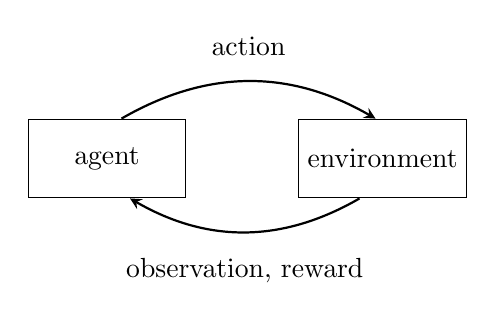
\begin{tikzpicture}[scale=1, transform shape, node distance=2.0cm]
\node (agent) [rec] {agent};
\node (environment) [rec, right of=agent, xshift=1.5cm] {environment};
\draw [arrow, xshift=0.5cm]  (environment.240) to [bend left=30] node [midway, below, yshift=-0.2cm] (textnode1) {observation, reward}  (agent.300);
\draw [arrow, xshift=0.5cm]  (agent.70) to [bend left=30] node [midway, above, yshift=0.2cm] (textnode2) {action} (environment.100);
\end{tikzpicture}
\end{center}
%\caption{Conceptual schematic of reinforcement learning.}
\label{fig:rl-shematic}
\end{figure}
\end{columns}
\end{frame}


\begin{frame}{Markov chain}
\begin{figure}[htpb]
\begin{center}
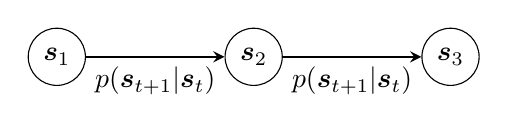
\begin{tikzpicture}[scale=1, transform shape, node distance=1.5cm]
		\node (s1) [mcs] {$\bm{s}_{1} $};
		\node (s2) [mcs, right of=s1, xshift=1cm] { $ \bm{s}_{2}  $};
		\draw [arrow] (s1) -- node [below, midway] {$ p(\bm{s}_{t+1}|\bm{s}_{t}) $} (s2);
		\node (s3) [mcs, right of=s2, xshift=1cm] { $ \bm{s}_{3}  $};
		\draw [arrow] (s2) -- node [below, midway] {$ p(\bm{s}_{t+1}|\bm{s}_{t}) $} (s3);
\end{tikzpicture}
\end{center}
\caption{Schematic of a Markov chain.}
\label{fig:markov-chain}
\end{figure}
\end{frame}


\begin{frame}{Markov decision process}
\begin{figure}[htpb]
\begin{center}
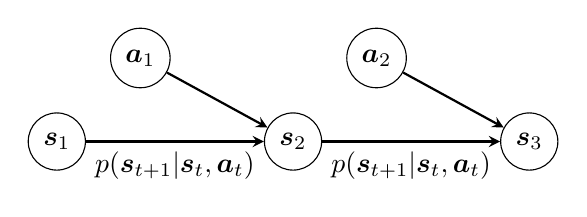
\begin{tikzpicture}[scale=1, transform shape, node distance=1.5cm]
		\node (s1) [mcs] {$\bm{s}_{1} $};
		\node (a1) [mcs, above right of=s1] { $ \bm{a}_{1}  $};
		\node (s2) [mcs, right of=s1, xshift=1.5cm] { $ \bm{s}_{2}  $};
		\draw [arrow] (a1) -- (s2);
		\draw [arrow] (s1) -- node [below, midway] {$ p(\bm{s}_{t+1}|\bm{s}_{t}, \bm{a}_{t}) $} (s2);
		\node (s3) [mcs, right of=s2, xshift=1.5cm] { $ \bm{s}_{3}  $};
		\node (a2) [mcs, above right of=s2] { $ \bm{a}_{2}  $};
		\draw [arrow] (s2) -- node [below, midway] {$ p(\bm{s}_{t+1}|\bm{s}_{t}, \bm{a}_{t}) $} (s3);
		\draw [arrow] (a2) -- (s3);
\end{tikzpicture}
\end{center}
\caption{Schematic of a Markov decision process.}
\label{fig:mdp}
\end{figure}
\end{frame}


\begin{frame}{Partially observable Markov decision processes}
\begin{figure}[htpb]
\begin{center}
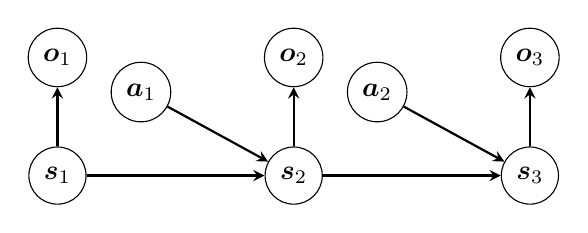
\begin{tikzpicture}[scale=1, transform shape, node distance=1.5cm]
		\node (s1) [mcs] {$\bm{s}_{1} $};
		\node (a1) [mcs, above right of=s1] { $ \bm{a}_{1}  $};
		\node (o1) [mcs, above of=s1] { $ \bm{o}_{1}  $};
		\draw [arrow] (s1) -- (o1);
		\node (s2) [mcs, right of=s1, xshift=1.5cm] { $ \bm{s}_{2}  $};
		\node (o2) [mcs, above of=s2] { $ \bm{o}_{2}  $};
		\draw [arrow] (s2) -- (o2);
		\draw [arrow] (a1) -- (s2);
		\draw [arrow] (s1) --  (s2);
		\node (s3) [mcs, right of=s2, xshift=1.5cm] { $ \bm{s}_{3}  $};
		\node (o3) [mcs, above of=s3] { $ \bm{o}_{3}  $};
		\draw [arrow] (s3) -- (o3);
		\node (a2) [mcs, above right of=s2] { $ \bm{a}_{2}  $};
		\draw [arrow] (s2) -- (s3);
		\draw [arrow] (a2) -- (s3);
\end{tikzpicture}
\end{center}
\caption{Schematic of a partially observable Markov decision process.}
\label{fig:pomdp}
\end{figure}

\end{frame}

\begin{frame}{Markov decision process with a policy}
\begin{figure}[htpb]
\begin{center}
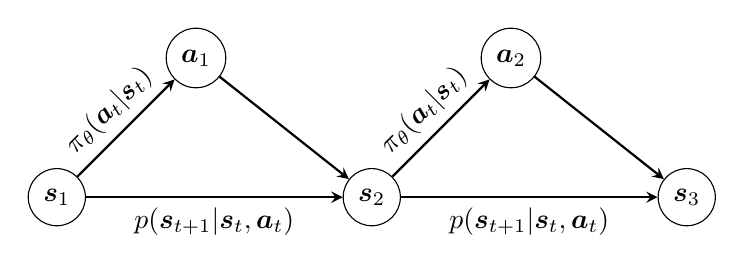
\begin{tikzpicture}[scale=1, transform shape, node distance=2.5cm]
		\node (s1) [mcs] {$\bm{s}_{1} $};
		\node (a1) [mcs, above right of=s1] { $ \bm{a}_{1}  $};
		\node (s2) [mcs, right of=s1, xshift=1.5cm] { $ \bm{s}_{2}  $};
		\draw [arrow] (a1) -- (s2);
		\draw [arrow] (s1) -- node [below, midway] {$ p(\bm{s}_{t+1}|\bm{s}_{t}, \bm{a}_{t}) $} (s2);
		\node (s3) [mcs, right of=s2, xshift=1.5cm] { $ \bm{s}_{3}  $};
		\node (a2) [mcs, above right of=s2] { $ \bm{a}_{2}  $};
		\draw [arrow] (s2) -- node [below, midway] {$ p(\bm{s}_{t+1}|\bm{s}_{t}, \bm{a}_{t}) $} (s3);
		\draw [arrow] (a2) -- (s3);
		\draw [arrow] (s1) -- node [above, midway, sloped] {$\pi_{ \theta } (\bm{a}_{t}| \bm{s}_{t} )  $} (a1);
		\draw [arrow] (s2) -- node [above, midway, sloped] {$\pi_{ \theta } (\bm{a}_{t}| \bm{s}_{t} )  $} (a2);
\end{tikzpicture}
\end{center}
\caption{Schematic of a Markov decision process with a policy $ \pi  $.}
\label{fig:policy-in-mdp}
\end{figure}
\end{frame}

\begin{frame}{Markov decision process in equation form}
\begin{equation*}
\underbrace{p_\theta(\bm{s}_1, \bm{a}_1, \dots, \bm{s}_T, \bm{a}_T)}_{p_\theta(\tau)} = p(\bm{s}_1) \prod^{T}_{t=1} 
\underbrace{\pi_{\theta} (\bm{a}_t | \bm{s}_t) p (\bm{s}_{t+1} | \bm{s}_t, \bm{a}_t)}_{\text{Markov chain on } (\bm{s}, \bm{a})}
\end{equation*}
		
\end{frame}

\begin{frame}{The goal of reinforcement learning}
Find policy parameters $ \theta^{ \star }  $ such that:
\begin{align*}
		\theta^\star &= \argmax_{\theta} \mathbb{E}_{\tau \sim p_\theta(\tau)} \left[ \sum_{t}^{} r(\bm{s}_t, \bm{a}_t) \right] \\
	 &= \argmax_{\theta} \sum_{t}^{T} \mathbb{E}_{(\bm{s}_t, \bm{a}_t) \sim p_\theta(\bm{s}_t, \bm{a}_t)} \left[  r(\bm{s}_t, \bm{a}_t) \right]
\end{align*}
\end{frame}

\begin{frame}{Value functions}
		Q-function:
\begin{equation*}
		\label{eq:q-function}
		Q^\pi (\bm{s}_t, \bm{a}_t) = \sum_{t'=t}^{T} \mathbb{E}_{\pi_\theta}
		\left[ r(\bm{s}_{t'}, \bm{a}_{t'} )| \bm{s}_t, \bm{a}_t \right] 
\end{equation*}
State value function:
\begin{equation*}
		\label{eq:value-function}
		V^\pi (\bm{s}_t) = \sum_{t'=t}^{T} \mathbb{E}_{\pi_\theta}
		\left[ r(\bm{s}_{t'}, \bm{a}_{t'} | \bm{s}_t) \right] 
\end{equation*}
Their connection:
\begin{equation*}
		V^\pi (\bm{s}_t) = \mathbb{E}_{\bm{a}_t \sim \pi(\bm{s}_t, \bm{a}_t)}
		\left[ Q^\pi(\bm{s}_t, \bm{a}_t) \right] 
\end{equation*}

\end{frame}

\begin{frame}{Classes of reinforcement learning algorithms}
		\underline{Based on objective}:
	\begin{itemize}
			\item policy gradient algorithms 
			\item actor-critic algorithms
			\item value iteration algorithms
	\end{itemize}
	\underline{Based on sampling strategy}:
	\begin{itemize}
			\item on-policy
			\item off-policy
	\end{itemize}
\end{frame}

\begin{frame}{Policy gradient algorithms}
\fbox{
		\parbox{\textwidth}{
				\underline{REINFORCE algorithm:}
\begin{enumerate}
		\item sample $\{\tau^i\}$ from $\pi_\theta(\bm{a}_t | \bm{s}_t)$ by running the policy
		\item use the samples to estimate the gradient of the objective: \newline $\nabla_\theta J(\theta) \approx   \sum_{i}^{} 
		\left ( \sum_{t}^{T} \nabla_\theta \log \pi_\theta (\bm{a}_{i,t} | \bm{s}_{i,t} ) \right )
		\left ( \sum_{t}^{} r(\bm{s}_{i,t}, \bm{a}_{i,t}) \right )$
\item update the policy function by performing a step of gradient ascent: \newline 
		$\theta \leftarrow \theta + \alpha \nabla_\theta J(\theta) $
\end{enumerate}
}}
		
\end{frame}


\begin{frame}{Actor critic algorithms}
\fbox{
\parbox{\textwidth}{
\underline{Actor-critic algorithm template}
\begin{enumerate}
		\item take action $\bm{a} \sim \pi_\theta(\bm{a}|\bm{s})$, observe transition
				$(\bm{s}, \bm{a},\bm{s'},r)$ and store it in the replay buffer $\mathcal{R}$ 
		\item sample a batch $\left\{  (\bm{s}_i, \bm{a}_i,\bm{s'}_i,r_i) \right\} $ from buffer $\mathcal{R}$
		\item update the Q-value estimator $\hat{Q}^\pi_\theta$ by using the target: \newline
				$y_i = r_i + \gamma \hat{Q}^\pi_\theta(\bm{s}_i', \bm{a}_i') \forall \bm{s}_i, \bm{a}_i$
		\item compute the policy gradient estimate with: \newline
				$\nabla_\theta J(\theta) \approx  \frac{1}{N} \sum_{i}^{}  \nabla_{\theta} \log \pi_\theta(\bm{a}^\pi_i|\bm{s}_i)\hat{Q}^\pi(\bm{s}_{i}, \bm{a}^\pi_{i})$,
				where $\bm{a}_i^\pi \sim \pi_\theta(\bm{a} | \bm{s}_i)$
		\item update the policy function by performing a gradient step: \newline
				$\theta \leftarrow \theta  + \alpha \nabla_\theta J(\theta)$
\end{enumerate}
}}
\end{frame}

\begin{frame}{epsilon-greedy policy}
\begin{equation}
		\label{eq-greedy-pi}
		\pi_{ \text{greedy} }(\bm{s}_{t}| \bm{a}_{t}) = \left\{ 
\begin{matrix}
		1 & \text{ if } \bm{a}_t = \argmax_{\bm{a}_t} A^\pi (\bm{s}_{t}, \bm{a}_{t}) 		 \\
		0 & \text{ otherwise}
\end{matrix}
		\right.
\end{equation}
\end{frame}

\begin{frame}{Value iteration}
Bootstrap update for the value function:
\begin{equation}
		\label{eq-bellman-value-update}
V^\pi(\bm{s}) \leftarrow E_{\bm{a} \sim \pi(\bm{a}|\bm{s})} \left[ r(\bm{s}_{}, \bm{a}_{}) + \gamma E_{\bm{s}' \sim p(\bm{s}' |\bm{a},\bm{s}  )} [V^\pi(\bm{s}') ] \right] 
\end{equation}

\fbox{
\parbox{\textwidth}{
		\label{alg-finite-value-iteration}
\underline{Value iteration}
\begin{enumerate}
		\item set $Q(\bm{s}, \bm{a}) \leftarrow r (\bm{s}, \bm{a}) + \gamma E[V(\bm{s}')]$
		\item set $V(\bm{s}) \leftarrow \max_{\bm{a}} Q(\bm{s}, \bm{a})$
\end{enumerate}
}}

\end{frame}

\begin{frame}{DQN}
\fbox{
\parbox{\textwidth}{
		\label{alg-classic-dqn}
\underline{``Classic'' DQN}
\begin{enumerate}
		\item take some action $\bm{a}_i$,  observe $\left( \bm{s}_i, \bm{a}_i, \bm{s}_i', r_i \right)$ and add it to $\mathcal{B}$
		\item sample a mini-batch  $\left( \bm{s}_j, \bm{a}_j, \bm{s}_j', r_j \right)$  from $\mathcal{B}$ uniformly
		\item compute $y_j = r_j + \gamma \max_{\bm{a}_j'} Q_{\phi'} (\bm{s}_{j}', \bm{a}_{j}')$ using the \textit{target} network $Q_{\phi'}$
		\item $  \phi \leftarrow \phi  - \alpha \sum_{j}^{}  \frac{d Q_\phi}{d\phi} (\bm{s}_{j}, \bm{a}_{j}) \left( Q_\phi(\bm{s}_{i}, \bm{a}_{i}) - 
				y_j 	\right) $ 
		\item update $\phi'$: copy $\phi$ every $N$ steps
\end{enumerate}
}}
		
\end{frame}

\begin{frame}{Rainbow}
DQN with the following improvements:
\begin{itemize}
		\item double Q-networks 
		\item multi-step returns
		\item prioritized replay buffer
		\item dueling network
		\item noisy networks
\end{itemize}
\end{frame}


\section{Representation learning} 

\begin{frame}{General remarks}
		\begin{itemize}
				\item goal is to learn a parametric mapping from raw input data
						to a feature vector in order to capture and extract useful
						abstract information
				\item works with unsupervised learning 
				\item generative and discriminative models
		\end{itemize}
\end{frame}

\begin{frame}{Generative models}
		\begin{itemize}
				\item deterministic:
						\begin{itemize}
								\item autoencoders (AEs)
						\end{itemize}
				\item probabilistic:
						\begin{itemize}
								\item variational autoencoders (VAEs)
								\item generative adversarial networks (GANs)
						\end{itemize}
		\end{itemize}
\end{frame}

\begin{frame}{Discriminative models}
		\begin{itemize}
				\item have only encoders
				\item trained with:
						\begin{itemize}
								\item contrastive learning
								\item bootstrapping
								\item ...
						\end{itemize}
		\end{itemize}
\end{frame}


\begin{frame}{Regularization for autoencoders}
		Known from \cite{bengio2013representation}, \cite{ghosh2019variational} and others:
		\begin{itemize}
				\item on input: 
						\begin{itemize}
								\item denoising autoencoders
						\end{itemize}
				\item on bottleneck:
						\begin{itemize}
								\item noise injection
								\item Tikhonov regularization (L2 regularization)
						\end{itemize}
				\item other:
						\begin{itemize}
								\item gradient penalty (weight decay)
								\item spectral normalization
						\end{itemize}
		\end{itemize}
\end{frame}


\section{Representation learning for control} 

\begin{frame}{Desirable properties}
		On top of general desirable properties for representations:
		\begin{itemize}
				\item having the Markov property
				\item represent states well enough for policy improvement
				\item generalize in the stateful sense
%				\item be low dimensional
		\end{itemize}
\end{frame}


\begin{frame}{Types of models}
		\begin{itemize}
				\item autoencoders
				\item forward models
				\item inverse models
				\item hybrid models
		\end{itemize}
\end{frame}


\begin{frame}{Autoencoders}
\begin{figure}[htpb]
\begin{center}
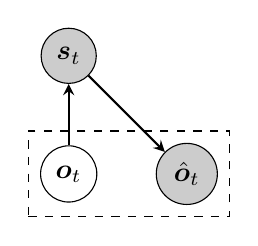
\begin{tikzpicture}[scale=1, transform shape, node distance=1.5cm]
		\node (st) [mcsb] {$\bm{s}_{t} $};
		\node (ot) [mcs, below of=st] {$\bm{o}_{t}$};
		\node (othat) [mcsb, right of=ot] {$\hat{\bm{o}}_{t} $};
		\draw [arrow] (ot) -- (st);
		\draw [arrow] (st) -- (othat);
		\node[draw,dashed,inner sep=1.5mm,fit=(ot) (othat) ] {};
\end{tikzpicture}
\end{center}
		\caption{Auto-encoder: learned by reconstructing the observation (one-to-one).
				The observation is the input and the computed state is the vector at
				the auto-encoder's bottleneck layer.}
\end{figure}
\end{frame}


\begin{frame}{Forward models}
\begin{figure}[htpb]
\begin{center}
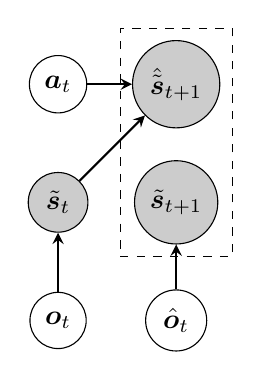
\begin{tikzpicture}[scale=1, transform shape, node distance=1.5cm]
		\node (at) [mcs] {$\bm{a}_{t} $};
		\node (st) [mcsb, below of=at] {$\tilde{\bm{s}}_{t} $};
		\node (sthatplus1) [mcsb, right of=at] {$\hat{\tilde{\bm{s}}}_{t+1} $};
		\node (stplus1) [mcsb, right of=st] {$\tilde{\bm{s}}_{t+1} $};
		\node (ot) [mcs, below of=st] {$\bm{o}_{t}$};
		\node (otplus1) [mcs, right of=ot] {$\hat{\bm{o}}_{t} $};
		\draw [arrow] (at) -- (sthatplus1);
		\draw [arrow] (st) -- (sthatplus1);
		\draw [arrow] (ot) -- (st);
		\draw [arrow] (otplus1) -- (stplus1);
		\node[draw,dashed,inner sep=1.5mm,fit=(sthatplus1) (stplus1) ] {};
\end{tikzpicture}
\end{center}
		\caption{Forward model: predicting the future state from the state-action pair.
				}
\end{figure}
\end{frame}


\begin{frame}{Inverse models}
\begin{figure}[htpb]
\begin{center}
\begin{tikzpicture}[scale=1, transform shape, node distance=1.5cm]
		\node (at) [mcs] {$\bm{a}_{t} $};
		\node (athat) [mcsb, below of=at] {$\hat{\bm{a}}_{t} $};
		\node (nothing) [below of=st] {};
		\node (sttilde) [mcsb, left of=nothing] {$\tilde{\bm{s}}_{t} $};
		\node (stildetplus1) [mcsb, right of=nothing] {$\tilde{\bm{s}}_{t+1} $};
		\node (ot) [mcs, below of=sttilde] {$\bm{o}_{t}$};
		\node (otplus1) [mcs, below of=stildetplus1] {$\bm{o}_{t+1} $};
		\draw [arrow] (ot) -- (sttilde);
		\draw [arrow] (otplus1) -- (stildetplus1);
		\draw [arrow] (sttilde) -- (athat);
		\draw [arrow] (stildetplus1) -- (athat);
		\node[draw,dashed,inner sep=1.5mm,fit=(at) (athat) ] {};
\end{tikzpicture}
\end{center}
		\caption{Inverse model: predicting the action between two consecutive states.
				}
\end{figure}
\end{frame}


\section{Related work} 

\begin{frame}{Reinforcement learning on Atari games}
		\begin{itemize}
				\item started with DQN \cite{mnih2013atari}
				\item many improvements:
				\begin{itemize}
						\item algorithm fundamentals, combination in \cite{rainbow}
						\item exploration schemes: \cite{icm}, \cite{ecoffet2021first}
						\item better sampling: \cite{andrychowicz2017hindsight},
								\cite{kapturowski2018recurrent}
				\end{itemize}
		\item model based algorithms: \cite{schrittwieser2020mastering}
				\item all solved on human level in \cite{agent57}
%				\item leveraging unsupervised state representation learning
		\end{itemize}

	\pause % Automatically creates a new "page" split between the above and above + below
	\begin{alertblock}{Next challenge}
		Making reinforcement learning \alert{more sample-efficient}.
	\end{alertblock}
		
\end{frame}

\begin{frame}{Using data augmentation for regularization}
	\begin{itemize}
			\item simply adding data augmentation to RL: \cite{rad}
			\item using it to regularize RL: \cite{drqv1}, \cite{drqv2}
	\end{itemize}	
\end{frame}


\begin{frame}{Leveraging unsupervised representation learning}
	\begin{itemize}
			\item early efforts for state representation learning did not work well
			\item initially used to help exploration:
\cite{lossisitsownreward}, \cite{rlwauxloss} or \cite{icm}
\item recent efforts use both deterministic and stochastic generative models (mostly
		stochastic)
\item most recent works focus on using discriminative models 
\item ideally obtained solely via pretrainining; recent efforts include 
		\cite{seo2022reinforcement}
	\end{itemize}	
\end{frame}

\begin{frame}{Deterministic generative models}
	Idea introduced in \cite{lange2010deep}.
	Most importantly used in \cite{sac+ae}.
	Authors identify the following for success:
	\begin{itemize}
			\item only value function gradients update the encoder
			\item same update rate for autoencoder and RL updates
			\item using L2 regularization
	\end{itemize}
	Possible improvements:
	\begin{itemize}
			\item prediction architecture from \cite{oh2015action}
			\item optical or latent flow: \cite{flow}
	\end{itemize}
\end{frame}


\begin{frame}{Stochastic generative models}
		Theoretically more interesting because:
		\begin{itemize}
				\item can be integrated into the underlying Markov chain: \cite{slac}
				\item can be used as models in model-based RL
		\end{itemize}
		Despite large interest they are hard to get to work due to 
		their stochasticity (elaborated and tested in \cite{sac+ae}).
\end{frame}


\begin{frame}{Discriminative models}
		More practical as there is no decoder (which is unnecessary for the purpose).
		Trained using different objectives:
		\begin{itemize}
				\item contrastive loss: \cite{curl}
				\item mutual information: \cite{rakelly2021mutual}, 
						\cite{anand2019unsupervised}, \cite{mazoure2020deep}
				\item bisimulation metrics: \cite{invariantrepwithoutreconstruction}
				\item bootstrapped self-predictions (introduced in \cite{grill2020bootstrap}):
\cite{schwarzer2020data}, and in \cite{merckling2022exploratory}
		\end{itemize}
\end{frame}

\section{Methods}

\begin{frame}{Our hypotheses}
		We want to test the following claims:
		\begin{enumerate}
				\item joint representation and reinforcement training 
						performs better than pretraining 
				\item representation better incentivised to learn stateful information
						will yield better features
				\item regularization is important for joint training stabilization
						and final effectiveness
		\end{enumerate}
		
\end{frame}

\begin{frame}{Implicit feature spaces hypothesis}

\begin{figure}[htpb]
\begin{center}

\def\setA{(1.0,0) circle (2)}%
\def\setB{(2.7,0) circle (1.5)}%
% define the bounding box
\def\boundb{(-5,3) rectangle (9,-3)}%
\begin{tikzpicture}[scale=0.75]
    \draw \boundb;
    % intersection
    \begin{scope}
    \clip \setA;
    \fill[black!20] \setB;
    \end{scope}
    \begin{scope}[even odd rule]% first circle without the second
    \clip \setB \boundb;
    \fill[red!20] \setA;
    \end{scope}
    \begin{scope}[even odd rule]% first circle without the second
    \clip \setA \boundb;
    \fill[blue!20] \setB;
    \end{scope}
    \draw \setA;
    \draw \setB;
    \node at (-1,0) [left, text width=2.5cm] {unsupervised learning (stateful noisy) features};
    \node at (5,0) [right, text width=2.5cm] {reinforcement learning (stateful) features};
	\node at (11,3) [below left, text width=7cm] {\underline{latent representation space}};
\end{tikzpicture}
\end{center}
\caption{Schematic of the latent representation space. }
\label{fig-rl-srl-features-space}
\end{figure}
\end{frame}


\begin{frame}{Testing hypothesis 1}
We can only indirectly test the hypothesis by observing the obtained returns
on different games. We run the following experiments and observe the results:
\begin{enumerate}
		\item only RL
		\item only RL, but on encoders from a finished RL run
		\item only RL, but on encoders pretrained with pixel reconstruction loss
		\item joint training from scratch
\end{enumerate}
\end{frame}


\begin{frame}{Testing hypothesis 2}
\begin{enumerate}
		\item joint training where unsupervised learning task is only compression
		\item joint training where unsupervised learning task is compression 
				and one-step forward prediction in pixel space
\end{enumerate}
\end{frame}


\begin{frame}{Testing hypothesis 3}
\begin{enumerate}
		\item joint training with no regularization
		\item joint training with L2 regularization
		\item joint training with L2 regularization and data augmentation
\end{enumerate}
\end{frame}


\begin{frame}{Module implementation}
We really implement our add-on module as an add-on module in 
the reinforcement learning library Tianshou. \\
This is possible because Tianshou abstract different parts of reinforcement learning.\\
We implement our module as a policy wrapper.
\end{frame}

\begin{frame}{Tianshou abstractions}
\begin{figure}[htpb]
		\centering
		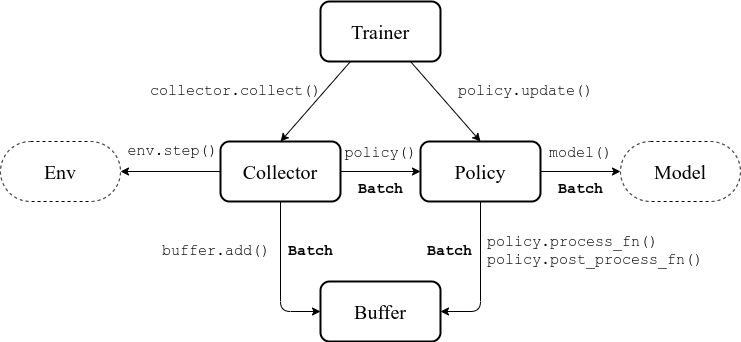
\includegraphics[width=0.8\textwidth]{"../thesis_text/figure/concepts_arch2.png"}
		\caption{Tianshou abstractions.}
		\label{tianshouconcepts}
\end{figure}
\end{frame}

\begin{frame}{Network architectures and hyperparameters}
\begin{itemize}
\item all reinforcement learning parameters are kept equal and correspond 
		to those in \cite{rainbow}
\item two sized encoders, 2-D convolutional layers specified as\\
		(number of input channels, number of output
channels, kernel size, stride, padding):
		\begin{itemize}
				\item smaller, same as in \cite{mnih2015humanlevel}: \\
(number of stacked frames, 32, 8, 4, 0), (32, 64, 4, 2, 0), (64, 64, 3, 1, 0)
\item bigger, same as in \cite{sac+ae}:\\
(number of stacked frames, 32, 3, 2, 0), 
(32, 32, 3, 2, 0),
(32, 32, 3, 2, 0),
(32, 32, 3, 2, 0) \\
followed by a linear layer of shape ($32 \times 35 \times 35$, features dimension)
		\end{itemize}
\end{itemize}
\end{frame}

\section{Results}

\begin{frame}{Games}
\begin{enumerate}
		\item Breakout
		\item Enduro
		\item Ms Pacman
		\item Pong
		\item Qbert
		\item Seaquest
		\item Space Invaders
\end{enumerate}
\end{frame}


\begin{frame}[plain]
		\centering
		\underline{Effectiveness of pretraining}
		\vspace{-1cm}
\begin{figure}[!t]
  \captionsetup[subfloat]{position=top,labelformat=empty}
  \centering
    \subfloat[]{  \resizebox{0.4\textwidth}{!}{
%\definecolor{blue}{RGB}{76,100,135}
%\definecolor{red}{RGB}{153,0,0}
%\definecolor{yellow}{RGB}{227,178,60}
%\definecolor{mycolor1}{rgb}{0.00000,0.44700,0.74100}%
%\definecolor{mycolor2}{rgb}{0.85000,0.32500,0.09800}%
%\definecolor{mycolor3}{rgb}{0.92900,0.69400,0.12500}%
%
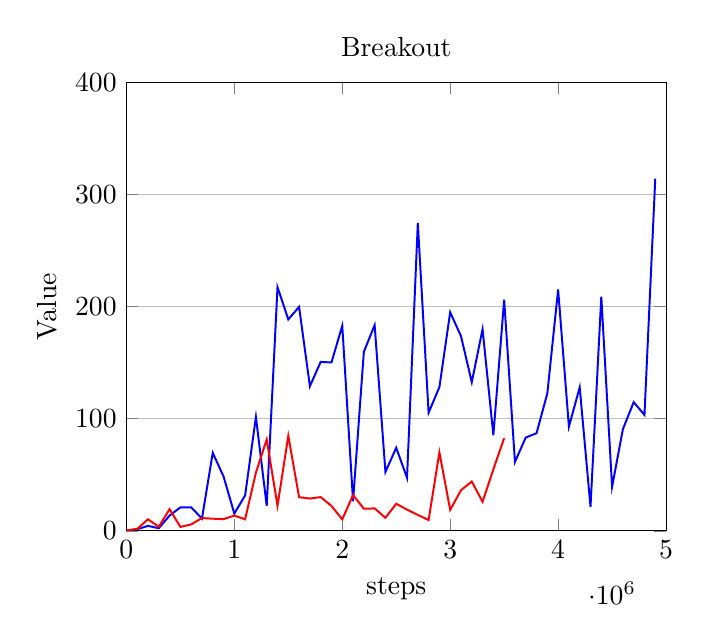
\begin{tikzpicture}

\begin{axis}[%
legend entries={rl-only-small-net,L2-reg,parallel-fs-50-no-aug}, 
legend columns=2,
title=Breakout,
legend to name=named,
legend style={legend cell align=left},
%%width=10in,
%%height=5in,
%%at={(2.596in,2.358in)},
% scale only axis,
xmin=0,
xmax=5000000,
xlabel style={font=\color{white!15!black}},
xlabel={steps},
xlabel near ticks,
ymin=0,
ymax=400,
ylabel style={font=\color{white!15!black}},
ylabel={Value},
ylabel near ticks,
ymajorgrids,
% %scale=0.5,
%%scale=0.4,
axis background/.style={fill=white},
%legend columns=2,
%legend=south outside
]
\addplot [color=blue, line width = 0.25mm]
                table[row sep=crcr]{
                  0 0.20000000298023224\\ 
100000 1.399999976158142\\ 
200000 4.400000095367432\\ 
300000 2.299999952316284\\ 
400000 13.600000381469727\\ 
500000 20.899999618530273\\ 
600000 21.0\\ 
700000 10.899999618530273\\ 
800000 69.5999984741211\\ 
900000 48.5\\ 
1000000 15.399999618530273\\ 
1100000 31.600000381469727\\ 
1200000 101.5999984741211\\ 
1300000 22.399999618530273\\ 
1400000 217.39999389648438\\ 
1500000 188.60000610351562\\ 
1600000 199.8000030517578\\ 
1700000 129.0\\ 
1800000 150.6999969482422\\ 
1900000 150.1999969482422\\ 
2000000 183.0\\ 
2100000 26.399999618530273\\ 
2200000 159.6999969482422\\ 
2300000 183.5\\ 
2400000 52.5\\ 
2500000 74.0999984741211\\ 
2600000 47.29999923706055\\ 
2700000 274.6000061035156\\ 
2800000 105.4000015258789\\ 
2900000 128.1999969482422\\ 
3000000 195.0\\ 
3100000 173.6999969482422\\ 
3200000 132.60000610351562\\ 
3300000 179.89999389648438\\ 
3400000 85.19999694824219\\ 
3500000 206.1999969482422\\ 
3600000 61.5\\ 
3700000 83.19999694824219\\ 
3800000 87.0999984741211\\ 
3900000 122.5999984741211\\ 
4000000 215.3000030517578\\ 
4100000 92.9000015258789\\ 
4200000 128.0\\ 
4300000 21.399999618530273\\ 
4400000 208.89999389648438\\ 
4500000 39.20000076293945\\ 
4600000 90.5999984741211\\ 
4700000 114.80000305175781\\ 
4800000 103.4000015258789\\ 
4900000 314.20001220703125\\ 
};
\addplot [color=red, line width = 0.25mm]
                table[row sep=crcr]{
                  0 0.4000000059604645\\ 
100000 1.7000000476837158\\ 
200000 10.300000190734863\\ 
300000 3.5999999046325684\\ 
400000 19.299999237060547\\ 
500000 3.5\\ 
600000 5.699999809265137\\ 
700000 11.399999618530273\\ 
800000 10.800000190734863\\ 
900000 10.399999618530273\\ 
1000000 13.600000381469727\\ 
1100000 10.300000190734863\\ 
1200000 51.900001525878906\\ 
1300000 81.5\\ 
1400000 22.299999237060547\\ 
1500000 84.69999694824219\\ 
1600000 30.0\\ 
1700000 28.799999237060547\\ 
1800000 30.100000381469727\\ 
1900000 22.200000762939453\\ 
2000000 10.199999809265137\\ 
2100000 31.899999618530273\\ 
2200000 19.700000762939453\\ 
2300000 20.0\\ 
2400000 11.600000381469727\\ 
2500000 24.200000762939453\\ 
2600000 18.899999618530273\\ 
2700000 14.199999809265137\\ 
2800000 9.600000381469727\\ 
2900000 70.0\\ 
3000000 18.700000762939453\\ 
3100000 36.20000076293945\\ 
3200000 44.0\\ 
3300000 25.899999618530273\\ 
3400000 54.900001525878906\\ 
3500000 82.69999694824219\\ 
};
\addplot [color=yellow, line width = 0.25mm]
                table[row sep=crcr]{
                  0 0.800000011920929\\ 
};
\end{axis}
\end{tikzpicture}}}
    \subfloat[]{  \resizebox{0.4\textwidth}{!}{
%\definecolor{blue}{RGB}{76,100,135}
%\definecolor{red}{RGB}{153,0,0}
%\definecolor{yellow}{RGB}{227,178,60}
%\definecolor{mycolor1}{rgb}{0.00000,0.44700,0.74100}%
%\definecolor{mycolor2}{rgb}{0.85000,0.32500,0.09800}%
%\definecolor{mycolor3}{rgb}{0.92900,0.69400,0.12500}%
%
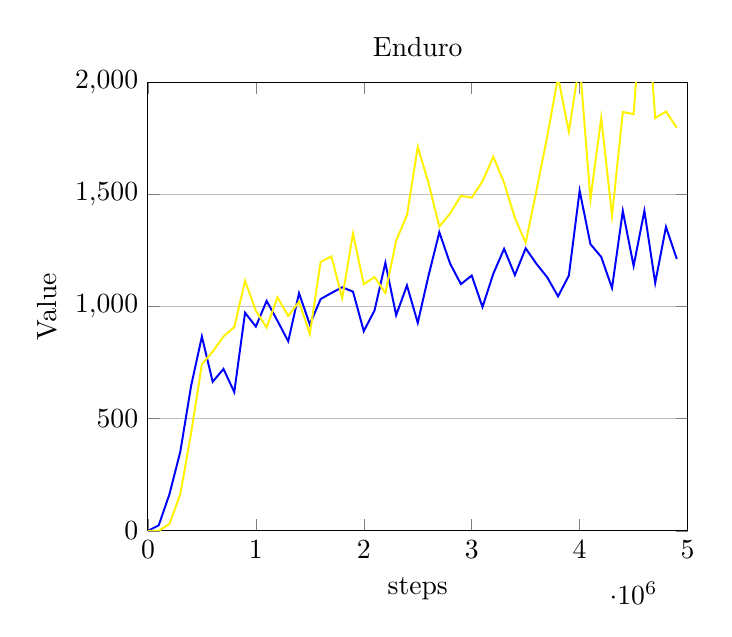
\begin{tikzpicture}

\begin{axis}[%
title=Enduro,
% %width=4.634in,
%%width=10in,
%%height=5in,
%at={(2.596in,2.358in)},
% scale only axis,
xmin=0,
xmax=5000000,
xlabel style={font=\color{white!15!black}},
xlabel={steps},
xlabel near ticks,
ymin=0,
ymax=2000,
ylabel style={font=\color{white!15!black}},
ylabel={Value},
ylabel near ticks,
ymajorgrids,
% %scale=0.5,
%scale=0.4,
axis background/.style={fill=white},
%legend style={legend cell align=left, align=left, draw=white!15!black}
]
\addplot [color=blue, line width = 0.25mm]
                table[row sep=crcr]{
                  0 0.0\\ 
100000 24.299999237060547\\ 
200000 164.3000030517578\\ 
300000 353.0\\ 
400000 646.4000244140625\\ 
500000 866.7000122070312\\ 
600000 664.7000122070312\\ 
700000 722.2000122070312\\ 
800000 618.9000244140625\\ 
900000 972.7999877929688\\ 
1000000 910.9000244140625\\ 
1100000 1025.699951171875\\ 
1200000 937.0\\ 
1300000 845.5999755859375\\ 
1400000 1059.9000244140625\\ 
1500000 920.2999877929688\\ 
1600000 1033.800048828125\\ 
1700000 1061.0\\ 
1800000 1086.5999755859375\\ 
1900000 1066.9000244140625\\ 
2000000 890.9000244140625\\ 
2100000 983.5\\ 
2200000 1195.300048828125\\ 
2300000 962.0\\ 
2400000 1094.800048828125\\ 
2500000 928.0\\ 
2600000 1138.5999755859375\\ 
2700000 1332.300048828125\\ 
2800000 1191.800048828125\\ 
2900000 1100.5999755859375\\ 
3000000 1138.800048828125\\ 
3100000 998.2999877929688\\ 
3200000 1146.800048828125\\ 
3300000 1258.0999755859375\\ 
3400000 1141.0\\ 
3500000 1260.300048828125\\ 
3600000 1190.800048828125\\ 
3700000 1130.5999755859375\\ 
3800000 1046.0999755859375\\ 
3900000 1138.4000244140625\\ 
4000000 1517.5\\ 
4100000 1278.9000244140625\\ 
4200000 1221.699951171875\\ 
4300000 1083.199951171875\\ 
4400000 1426.9000244140625\\ 
4500000 1181.5999755859375\\ 
4600000 1427.199951171875\\ 
4700000 1105.800048828125\\ 
4800000 1355.800048828125\\ 
4900000 1212.9000244140625\\ 
};
\addplot [color=red, line width = 0.25mm]
                table[row sep=crcr]{
                  0 0.0\\ 
};
\addplot [color=yellow, line width = 0.25mm]
                table[row sep=crcr]{
                  0 0.0\\ 
100000 0.0\\ 
200000 30.700000762939453\\ 
300000 163.6999969482422\\ 
400000 435.79998779296875\\ 
500000 743.2000122070312\\ 
600000 799.2000122070312\\ 
700000 867.0\\ 
800000 908.4000244140625\\ 
900000 1115.300048828125\\ 
1000000 981.4000244140625\\ 
1100000 906.9000244140625\\ 
1200000 1041.5999755859375\\ 
1300000 958.5999755859375\\ 
1400000 1021.9000244140625\\ 
1500000 877.7000122070312\\ 
1600000 1199.4000244140625\\ 
1700000 1224.0\\ 
1800000 1038.199951171875\\ 
1900000 1326.0999755859375\\ 
2000000 1100.0\\ 
2100000 1132.0999755859375\\ 
2200000 1060.9000244140625\\ 
2300000 1294.300048828125\\ 
2400000 1407.699951171875\\ 
2500000 1712.5\\ 
2600000 1551.5\\ 
2700000 1357.0\\ 
2800000 1415.800048828125\\ 
2900000 1494.5\\ 
3000000 1486.0\\ 
3100000 1559.699951171875\\ 
3200000 1668.5\\ 
3300000 1552.800048828125\\ 
3400000 1395.800048828125\\ 
3500000 1284.9000244140625\\ 
3600000 1518.0\\ 
3700000 1759.5999755859375\\ 
3800000 2024.9000244140625\\ 
3900000 1780.0999755859375\\ 
4000000 2090.5\\ 
4100000 1479.0999755859375\\ 
4200000 1841.699951171875\\ 
4300000 1405.5999755859375\\ 
4400000 1868.300048828125\\ 
4500000 1858.699951171875\\ 
4600000 2527.0\\ 
4700000 1841.0\\ 
4800000 1870.800048828125\\ 
4900000 1797.9000244140625\\ 
};
\end{axis}
\end{tikzpicture}}}\\
  \vspace{-1cm}
    \subfloat[]{  \resizebox{0.4\textwidth}{!}{
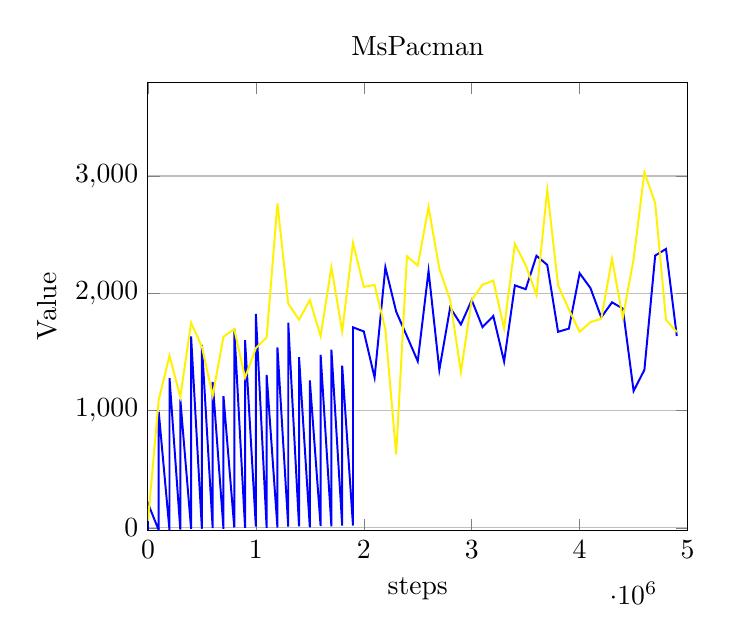
\begin{tikzpicture}

\begin{axis}[%
title=MsPacman,
% %width=4.634in,
%width=10in,
%height=5in,
%at={(2.596in,2.358in)},
% scale only axis,
xmin=0,
xmax=5000000,
xlabel style={font=\color{white!15!black}},
xlabel={steps},
xlabel near ticks,
ymin=-22,
ymax=3800,
ylabel style={font=\color{white!15!black}},
ylabel={Value},
ylabel near ticks,
ymajorgrids,
% %scale=0.5,
%scale=0.4,
axis background/.style={fill=white},
%legend style={legend cell align=left, align=left, draw=white!15!black}
]
\addplot [color=blue, line width = 0.25mm]
                table[row sep=crcr]{
                  0 -21.0\\ 
0 210.0\\ 
100000 -19.799999237060547\\ 
100000 990.0\\ 
200000 -20.700000762939453\\ 
200000 1277.0\\ 
300000 -15.0\\ 
300000 1096.0\\ 
400000 -7.0\\ 
400000 1632.0\\ 
500000 -6.900000095367432\\ 
500000 1561.0\\ 
600000 -1.899999976158142\\ 
600000 1245.0\\ 
700000 -7.599999904632568\\ 
700000 1123.0\\ 
800000 4.0\\ 
800000 1696.0\\ 
900000 1.5\\ 
900000 1600.0\\ 
1000000 11.300000190734863\\ 
1000000 1824.0\\ 
1100000 1.2000000476837158\\ 
1100000 1304.0\\ 
1200000 3.700000047683716\\ 
1200000 1538.0\\ 
1300000 11.5\\ 
1300000 1750.0\\ 
1400000 13.600000381469727\\ 
1400000 1456.0\\ 
1500000 5.699999809265137\\ 
1500000 1258.0\\ 
1600000 15.600000381469727\\ 
1600000 1476.0\\ 
1700000 13.5\\ 
1700000 1519.0\\ 
1800000 19.299999237060547\\ 
1800000 1383.0\\ 
1900000 20.799999237060547\\ 
1900000 1710.0\\ 
2000000 1675.0\\ 
2100000 1282.0\\ 
2200000 2222.0\\ 
2300000 1844.0\\ 
2400000 1634.0\\ 
2500000 1421.0\\ 
2600000 2191.0\\ 
2700000 1347.0\\ 
2800000 1878.0\\ 
2900000 1735.0\\ 
3000000 1942.0\\ 
3100000 1712.0\\ 
3200000 1806.0\\ 
3300000 1419.0\\ 
3400000 2068.0\\ 
3500000 2035.0\\ 
3600000 2320.0\\ 
3700000 2242.0\\ 
3800000 1672.0\\ 
3900000 1699.0\\ 
4000000 2171.0\\ 
4100000 2045.0\\ 
4200000 1795.0\\ 
4300000 1923.0\\ 
4400000 1870.0\\ 
4500000 1167.0\\ 
4600000 1348.0\\ 
4700000 2322.0\\ 
4800000 2378.0\\ 
4900000 1636.0\\ 
};
\addplot [color=red, line width = 0.25mm]
                table[row sep=crcr]{
                  0 0.0\\ 
};
\addplot [color=yellow, line width = 0.25mm]
                table[row sep=crcr]{
                  0 60.0\\ 
100000 1090.0\\ 
200000 1469.0\\ 
300000 1117.0\\ 
400000 1749.0\\ 
500000 1545.0\\ 
600000 1128.0\\ 
700000 1630.0\\ 
800000 1695.0\\ 
900000 1281.0\\ 
1000000 1532.0\\ 
1100000 1625.0\\ 
1200000 2767.0\\ 
1300000 1912.0\\ 
1400000 1775.0\\ 
1500000 1942.0\\ 
1600000 1636.0\\ 
1700000 2222.0\\ 
1800000 1676.0\\ 
1900000 2430.0\\ 
2000000 2055.0\\ 
2100000 2072.0\\ 
2200000 1693.0\\ 
2300000 625.0\\ 
2400000 2317.0\\ 
2500000 2236.0\\ 
2600000 2736.0\\ 
2700000 2209.0\\ 
2800000 1944.0\\ 
2900000 1329.0\\ 
3000000 1944.0\\ 
3100000 2074.0\\ 
3200000 2109.0\\ 
3300000 1701.0\\ 
3400000 2421.0\\ 
3500000 2240.0\\ 
3600000 1986.0\\ 
3700000 2883.0\\ 
3800000 2069.0\\ 
3900000 1863.0\\ 
4000000 1672.0\\ 
4100000 1754.0\\ 
4200000 1783.0\\ 
4300000 2293.0\\ 
4400000 1791.0\\ 
4500000 2293.0\\ 
4600000 3033.0\\ 
4700000 2768.0\\ 
4800000 1774.0\\ 
4900000 1670.0\\ 
};
\end{axis}
\end{tikzpicture}}}
    \subfloat[]{  \resizebox{0.4\textwidth}{!}{
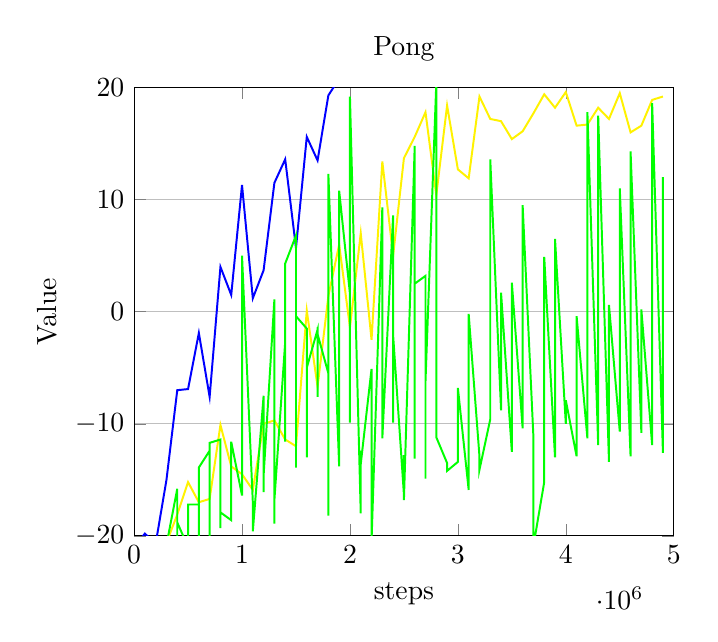
\begin{tikzpicture}

\begin{axis}[%
title=Pong,
% %width=4.634in,
%width=10in,
%height=5in,
%at={(2.596in,2.358in)},
% scale only axis,
xmin=0,
xmax=5000000,
xlabel style={font=\color{white!15!black}},
xlabel={steps},
xlabel near ticks,
ymin=-20,
ymax=20,
ylabel style={font=\color{white!15!black}},
ylabel={Value},
ylabel near ticks,
ymajorgrids,
% %scale=0.5,
%scale=0.4,
axis background/.style={fill=white},
%legend style={legend cell align=left, align=left, draw=white!15!black}
]
\addplot [color=blue, line width = 0.25mm]
                table[row sep=crcr]{
                  0 -21.0\\ 
100000 -19.799999237060547\\ 
200000 -20.700000762939453\\ 
300000 -15.0\\ 
400000 -7.0\\ 
500000 -6.900000095367432\\ 
600000 -1.899999976158142\\ 
700000 -7.599999904632568\\ 
800000 4.0\\ 
900000 1.5\\ 
1000000 11.300000190734863\\ 
1100000 1.2000000476837158\\ 
1200000 3.700000047683716\\ 
1300000 11.5\\ 
1400000 13.600000381469727\\ 
1500000 5.699999809265137\\ 
1600000 15.600000381469727\\ 
1700000 13.5\\ 
1800000 19.299999237060547\\ 
1900000 20.799999237060547\\ 
};
\addplot [color=red, line width = 0.25mm]
                table[row sep=crcr]{
                  0 0.0\\ 
};
\addplot [color=yellow, line width = 0.25mm]
                table[row sep=crcr]{
                  0 -21.0\\ 
0 -21.0\\ 
0 -21.0\\ 
100000 -21.0\\ 
200000 -20.299999237060547\\ 
300000 -20.600000381469727\\ 
400000 -18.100000381469727\\ 
500000 -15.199999809265137\\ 
600000 -17.0\\ 
700000 -16.700000762939453\\ 
800000 -10.100000381469727\\ 
900000 -13.800000190734863\\ 
1000000 -14.5\\ 
1100000 -15.899999618530273\\ 
1200000 -10.0\\ 
1300000 -9.699999809265137\\ 
1400000 -11.399999618530273\\ 
1500000 -12.0\\ 
1600000 0.10000000149011612\\ 
1700000 -6.699999809265137\\ 
1800000 1.399999976158142\\ 
1900000 6.0\\ 
2000000 -1.399999976158142\\ 
2100000 7.0\\ 
2200000 -2.5\\ 
2300000 13.399999618530273\\ 
2400000 5.0\\ 
2500000 13.699999809265137\\ 
2600000 15.600000381469727\\ 
2700000 17.799999237060547\\ 
2800000 10.399999618530273\\ 
2900000 18.399999618530273\\ 
3000000 12.699999809265137\\ 
3100000 11.899999618530273\\ 
3200000 19.200000762939453\\ 
3300000 17.200000762939453\\ 
3400000 17.0\\ 
3500000 15.399999618530273\\ 
3600000 16.100000381469727\\ 
3700000 17.700000762939453\\ 
3800000 19.399999618530273\\ 
3900000 18.200000762939453\\ 
4000000 19.600000381469727\\ 
4100000 16.600000381469727\\ 
4200000 16.700000762939453\\ 
4300000 18.200000762939453\\ 
4400000 17.200000762939453\\ 
4500000 19.5\\ 
4600000 16.0\\ 
4700000 16.600000381469727\\ 
4800000 18.899999618530273\\ 
4900000 19.200000762939453\\ 
};
\addplot [color=green, line width = 0.25mm]
                table[row sep=crcr]{
                  0 -21.0\\ 
0 -21.0\\ 
0 -21.0\\ 
0 -21.0\\ 
100000 -21.0\\ 
100000 -20.600000381469727\\ 
100000 -21.0\\ 
200000 -20.399999618530273\\ 
200000 -21.0\\ 
200000 -20.799999237060547\\ 
300000 -20.600000381469727\\ 
300000 -20.799999237060547\\ 
300000 -20.799999237060547\\ 
400000 -15.800000190734863\\ 
400000 -20.399999618530273\\ 
400000 -18.799999237060547\\ 
500000 -21.0\\ 
500000 -21.0\\ 
500000 -17.200000762939453\\ 
600000 -17.200000762939453\\ 
600000 -20.600000381469727\\ 
600000 -13.899999618530273\\ 
700000 -12.399999618530273\\ 
700000 -20.100000381469727\\ 
700000 -11.699999809265137\\ 
800000 -11.399999618530273\\ 
800000 -19.299999237060547\\ 
800000 -17.899999618530273\\ 
900000 -18.600000381469727\\ 
900000 -15.699999809265137\\ 
900000 -11.600000381469727\\ 
1000000 -16.399999618530273\\ 
1000000 -16.0\\ 
1000000 5.0\\ 
1100000 -17.0\\ 
1100000 -17.5\\ 
1100000 -19.600000381469727\\ 
1200000 -7.5\\ 
1200000 -16.100000381469727\\ 
1200000 -14.600000381469727\\ 
1300000 1.100000023841858\\ 
1300000 -18.899999618530273\\ 
1300000 -16.799999237060547\\ 
1400000 -2.700000047683716\\ 
1400000 -11.600000381469727\\ 
1400000 4.300000190734863\\ 
1500000 6.800000190734863\\ 
1500000 -13.899999618530273\\ 
1500000 -0.4000000059604645\\ 
1600000 -1.5\\ 
1600000 -13.0\\ 
1600000 -5.0\\ 
1700000 -1.600000023841858\\ 
1700000 -7.599999904632568\\ 
1700000 -2.0\\ 
1800000 -5.5\\ 
1800000 -18.200000762939453\\ 
1800000 12.300000190734863\\ 
1900000 -13.800000190734863\\ 
1900000 -10.0\\ 
1900000 10.800000190734863\\ 
2000000 1.600000023841858\\ 
2000000 -9.899999618530273\\ 
2000000 19.200000762939453\\ 
2100000 -18.0\\ 
2100000 -12.399999618530273\\ 
2100000 -13.600000381469727\\ 
2200000 -5.099999904632568\\ 
2200000 -13.899999618530273\\ 
2200000 -20.5\\ 
2300000 9.300000190734863\\ 
2300000 -8.199999809265137\\ 
2300000 -11.300000190734863\\ 
2400000 8.600000381469727\\ 
2400000 -9.899999618530273\\ 
2400000 -2.0999999046325684\\ 
2500000 -16.299999237060547\\ 
2500000 -12.800000190734863\\ 
2500000 -16.799999237060547\\ 
2600000 14.800000190734863\\ 
2600000 -13.100000381469727\\ 
2600000 2.5\\ 
2700000 3.200000047683716\\ 
2700000 -14.899999618530273\\ 
2700000 -6.199999809265137\\ 
2800000 20.399999618530273\\ 
2800000 -9.800000190734863\\ 
2800000 -11.199999809265137\\ 
2900000 -13.5\\ 
2900000 -14.199999809265137\\ 
3000000 -13.399999618530273\\ 
3000000 -6.800000190734863\\ 
3100000 -15.899999618530273\\ 
3100000 -0.20000000298023224\\ 
3200000 -12.899999618530273\\ 
3200000 -14.100000381469727\\ 
3300000 -9.600000381469727\\ 
3300000 13.600000381469727\\ 
3400000 -8.800000190734863\\ 
3400000 1.7000000476837158\\ 
3500000 -12.5\\ 
3500000 2.5999999046325684\\ 
3600000 -10.399999618530273\\ 
3600000 9.5\\ 
3700000 -11.199999809265137\\ 
3700000 -20.899999618530273\\ 
3800000 -15.199999809265137\\ 
3800000 4.900000095367432\\ 
3900000 -13.0\\ 
3900000 6.5\\ 
4000000 -10.0\\ 
4000000 -7.900000095367432\\ 
4100000 -12.899999618530273\\ 
4100000 -0.4000000059604645\\ 
4200000 -11.300000190734863\\ 
4200000 17.799999237060547\\ 
4300000 -11.899999618530273\\ 
4300000 17.5\\ 
4400000 -13.399999618530273\\ 
4400000 0.6000000238418579\\ 
4500000 -10.699999809265137\\ 
4500000 11.0\\ 
4600000 -12.899999618530273\\ 
4600000 14.300000190734863\\ 
4700000 -10.800000190734863\\ 
4700000 0.20000000298023224\\ 
4800000 -11.899999618530273\\ 
4800000 18.600000381469727\\ 
4900000 -12.600000381469727\\ 
4900000 12.0\\ 
};
\end{axis}
\end{tikzpicture}}}\\
    \ref{named}
%  \label{fig:rl-only-vs-pretrained}
\end{figure}
\end{frame}


\begin{frame}[plain]
%{Effectiveness of pretraining --- continued}
		\centering
		\underline{Effectiveness of pretraining --- continued}
		\vspace{-1cm}
\begin{figure}[!t]
  \captionsetup[subfloat]{position=top,labelformat=empty}
  \centering
    \subfloat[]{  \resizebox{0.4\textwidth}{!}{
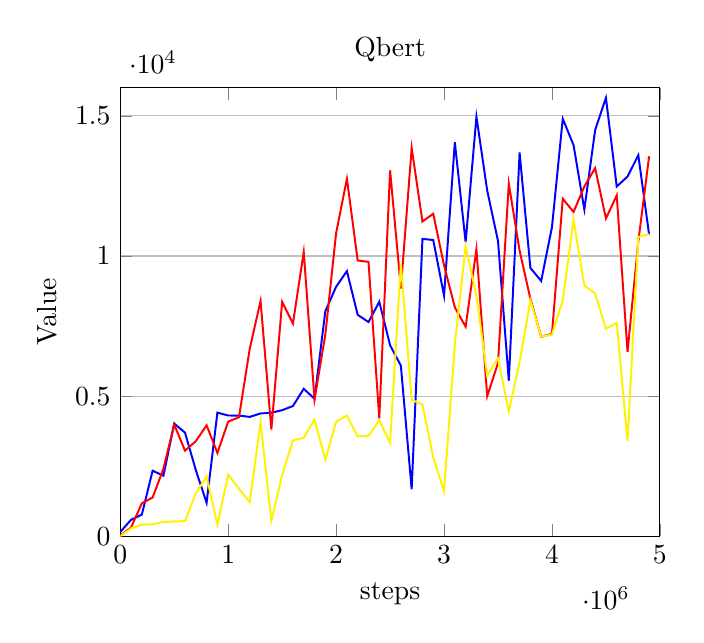
\begin{tikzpicture}

\begin{axis}[%
title=Qbert,
% %width=4.634in,
%width=10in,
%height=5in,
%at={(2.596in,2.358in)},
% scale only axis,
xmin=0,
xmax=5000000,
xlabel style={font=\color{white!15!black}},
xlabel={steps},
xlabel near ticks,
ymin=0,
ymax=16000,
ylabel style={font=\color{white!15!black}},
ylabel={Value},
ylabel near ticks,
ymajorgrids,
% %scale=0.5,
%scale=0.4,
axis background/.style={fill=white},
%legend style={legend cell align=left, align=left, draw=white!15!black}
]
\addplot [color=blue, line width = 0.25mm]
                table[row sep=crcr]{
                  0 150.0\\ 
100000 585.0\\ 
200000 772.5\\ 
300000 2337.5\\ 
400000 2157.5\\ 
500000 4022.5\\ 
600000 3695.0\\ 
700000 2362.5\\ 
800000 1192.5\\ 
900000 4410.0\\ 
1000000 4307.5\\ 
1100000 4305.0\\ 
1200000 4257.5\\ 
1300000 4380.0\\ 
1400000 4407.5\\ 
1500000 4497.5\\ 
1600000 4645.0\\ 
1700000 5260.0\\ 
1800000 4905.0\\ 
1900000 8030.0\\ 
2000000 8902.5\\ 
2100000 9460.0\\ 
2200000 7900.0\\ 
2300000 7642.5\\ 
2400000 8367.5\\ 
2500000 6815.0\\ 
2600000 6085.0\\ 
2700000 1677.5\\ 
2800000 10610.0\\ 
2900000 10570.0\\ 
3000000 8585.0\\ 
3100000 14057.5\\ 
3200000 10490.0\\ 
3300000 14970.0\\ 
3400000 12332.5\\ 
3500000 10537.5\\ 
3600000 5550.0\\ 
3700000 13692.5\\ 
3800000 9572.5\\ 
3900000 9110.0\\ 
4000000 11030.0\\ 
4100000 14897.5\\ 
4200000 13955.0\\ 
4300000 11660.0\\ 
4400000 14495.0\\ 
4500000 15645.0\\ 
4600000 12480.0\\ 
4700000 12835.0\\ 
4800000 13597.5\\ 
4900000 10762.5\\ 
};
\addplot [color=red, line width = 0.25mm]
                table[row sep=crcr]{
                  0 22.5\\ 
100000 310.0\\ 
200000 1172.5\\ 
300000 1382.5\\ 
400000 2410.0\\ 
500000 3982.5\\ 
600000 3052.5\\ 
700000 3390.0\\ 
800000 3957.5\\ 
900000 2970.0\\ 
1000000 4090.0\\ 
1100000 4245.0\\ 
1200000 6697.5\\ 
1300000 8395.0\\ 
1400000 3807.5\\ 
1500000 8360.0\\ 
1600000 7590.0\\ 
1700000 10142.5\\ 
1800000 4877.5\\ 
1900000 7190.0\\ 
2000000 10817.5\\ 
2100000 12755.0\\ 
2200000 9840.0\\ 
2300000 9790.0\\ 
2400000 4202.5\\ 
2500000 13057.5\\ 
2600000 8842.5\\ 
2700000 13852.5\\ 
2800000 11230.0\\ 
2900000 11507.5\\ 
3000000 9665.0\\ 
3100000 8167.5\\ 
3200000 7475.0\\ 
3300000 10242.5\\ 
3400000 4997.5\\ 
3500000 6180.0\\ 
3600000 12582.5\\ 
3700000 10190.0\\ 
3800000 8475.0\\ 
3900000 7115.0\\ 
4000000 7222.5\\ 
4100000 12042.5\\ 
4200000 11572.5\\ 
4300000 12480.0\\ 
4400000 13137.5\\ 
4500000 11337.5\\ 
4600000 12165.0\\ 
4700000 6580.0\\ 
4800000 10517.5\\ 
4900000 13560.0\\ 
};
\addplot [color=yellow, line width = 0.25mm]
                table[row sep=crcr]{
                  0 0.0\\ 
100000 280.0\\ 
200000 415.0\\ 
300000 425.0\\ 
400000 507.5\\ 
500000 525.0\\ 
600000 537.5\\ 
700000 1525.0\\ 
800000 2137.5\\ 
900000 407.5\\ 
1000000 2195.0\\ 
1100000 1690.0\\ 
1200000 1215.0\\ 
1300000 4077.5\\ 
1400000 550.0\\ 
1500000 2185.0\\ 
1600000 3417.5\\ 
1700000 3512.5\\ 
1800000 4165.0\\ 
1900000 2730.0\\ 
2000000 4090.0\\ 
2100000 4305.0\\ 
2200000 3557.5\\ 
2300000 3585.0\\ 
2400000 4137.5\\ 
2500000 3335.0\\ 
2600000 9722.5\\ 
2700000 4865.0\\ 
2800000 4700.0\\ 
2900000 2812.5\\ 
3000000 1605.0\\ 
3100000 6847.5\\ 
3200000 10342.5\\ 
3300000 8590.0\\ 
3400000 5732.5\\ 
3500000 6345.0\\ 
3600000 4447.5\\ 
3700000 6217.5\\ 
3800000 8415.0\\ 
3900000 7120.0\\ 
4000000 7195.0\\ 
4100000 8415.0\\ 
4200000 11307.5\\ 
4300000 8942.5\\ 
4400000 8662.5\\ 
4500000 7402.5\\ 
4600000 7612.5\\ 
4700000 3395.0\\ 
4800000 10680.0\\ 
4900000 10780.0\\ 
};
\end{axis}
\end{tikzpicture}}}
    \subfloat[]{  \resizebox{0.4\textwidth}{!}{
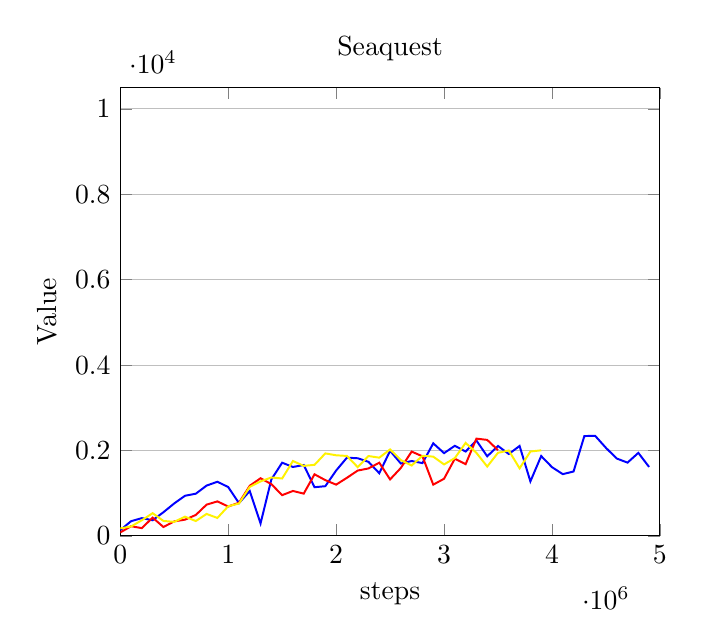
\begin{tikzpicture}

\begin{axis}[%
title=Seaquest,
% %width=4.634in,
%width=10in,
%height=5in,
%at={(2.596in,2.358in)},
% scale only axis,
xmin=0,
xmax=5000000,
xlabel style={font=\color{white!15!black}},
xlabel={steps},
xlabel near ticks,
ymin=0,
ymax=10500,
ylabel style={font=\color{white!15!black}},
ylabel={Value},
ylabel near ticks,
ymajorgrids,
% %scale=0.5,
%scale=0.4,
axis background/.style={fill=white},
%legend style={legend cell align=left, align=left, draw=white!15!black}
]
\addplot [color=blue, line width = 0.25mm]
                table[row sep=crcr]{
                  0 134.0\\ 
100000 344.0\\ 
200000 416.0\\ 
300000 366.0\\ 
400000 554.0\\ 
500000 760.0\\ 
600000 940.0\\ 
700000 988.0\\ 
800000 1178.0\\ 
900000 1268.0\\ 
1000000 1144.0\\ 
1100000 768.0\\ 
1200000 1052.0\\ 
1300000 292.0\\ 
1400000 1322.0\\ 
1500000 1714.0\\ 
1600000 1614.0\\ 
1700000 1660.0\\ 
1800000 1140.0\\ 
1900000 1164.0\\ 
2000000 1530.0\\ 
2100000 1832.0\\ 
2200000 1818.0\\ 
2300000 1734.0\\ 
2400000 1468.0\\ 
2500000 1992.0\\ 
2600000 1694.0\\ 
2700000 1754.0\\ 
2800000 1704.0\\ 
2900000 2168.0\\ 
3000000 1938.0\\ 
3100000 2110.0\\ 
3200000 1976.0\\ 
3300000 2234.0\\ 
3400000 1864.0\\ 
3500000 2106.0\\ 
3600000 1918.0\\ 
3700000 2106.0\\ 
3800000 1276.0\\ 
3900000 1870.0\\ 
4000000 1610.0\\ 
4100000 1446.0\\ 
4200000 1508.0\\ 
4300000 2338.0\\ 
4400000 2344.0\\ 
4500000 2062.0\\ 
4600000 1812.0\\ 
4700000 1716.0\\ 
4800000 1944.0\\ 
4900000 1614.0\\ 
};
\addplot [color=red, line width = 0.25mm]
                table[row sep=crcr]{
                  0 80.0\\ 
100000 226.0\\ 
200000 182.0\\ 
300000 428.0\\ 
400000 208.0\\ 
500000 340.0\\ 
600000 380.0\\ 
700000 490.0\\ 
800000 732.0\\ 
900000 808.0\\ 
1000000 688.0\\ 
1100000 776.0\\ 
1200000 1174.0\\ 
1300000 1350.0\\ 
1400000 1212.0\\ 
1500000 954.0\\ 
1600000 1052.0\\ 
1700000 990.0\\ 
1800000 1442.0\\ 
1900000 1306.0\\ 
2000000 1200.0\\ 
2100000 1360.0\\ 
2200000 1530.0\\ 
2300000 1580.0\\ 
2400000 1714.0\\ 
2500000 1322.0\\ 
2600000 1592.0\\ 
2700000 1974.0\\ 
2800000 1864.0\\ 
2900000 1200.0\\ 
3000000 1338.0\\ 
3100000 1808.0\\ 
3200000 1680.0\\ 
3300000 2278.0\\ 
3400000 2248.0\\ 
3500000 2008.0\\ 
};
\addplot [color=yellow, line width = 0.25mm]
                table[row sep=crcr]{
                  0 176.0\\ 
100000 220.0\\ 
200000 366.0\\ 
300000 532.0\\ 
400000 350.0\\ 
500000 328.0\\ 
600000 450.0\\ 
700000 348.0\\ 
800000 514.0\\ 
900000 420.0\\ 
1000000 694.0\\ 
1100000 758.0\\ 
1200000 1148.0\\ 
1300000 1276.0\\ 
1400000 1368.0\\ 
1500000 1344.0\\ 
1600000 1754.0\\ 
1700000 1640.0\\ 
1800000 1664.0\\ 
1900000 1932.0\\ 
2000000 1888.0\\ 
2100000 1872.0\\ 
2200000 1610.0\\ 
2300000 1870.0\\ 
2400000 1832.0\\ 
2500000 2024.0\\ 
2600000 1774.0\\ 
2700000 1648.0\\ 
2800000 1876.0\\ 
2900000 1856.0\\ 
3000000 1674.0\\ 
3100000 1822.0\\ 
3200000 2178.0\\ 
3300000 1944.0\\ 
3400000 1624.0\\ 
3500000 1946.0\\ 
3600000 2000.0\\ 
3700000 1582.0\\ 
3800000 1976.0\\ 
3900000 2004.0\\ 
};
\end{axis}
\end{tikzpicture}}}\\
  \vspace{-1cm}
    \subfloat[]{  \resizebox{0.4\textwidth}{!}{
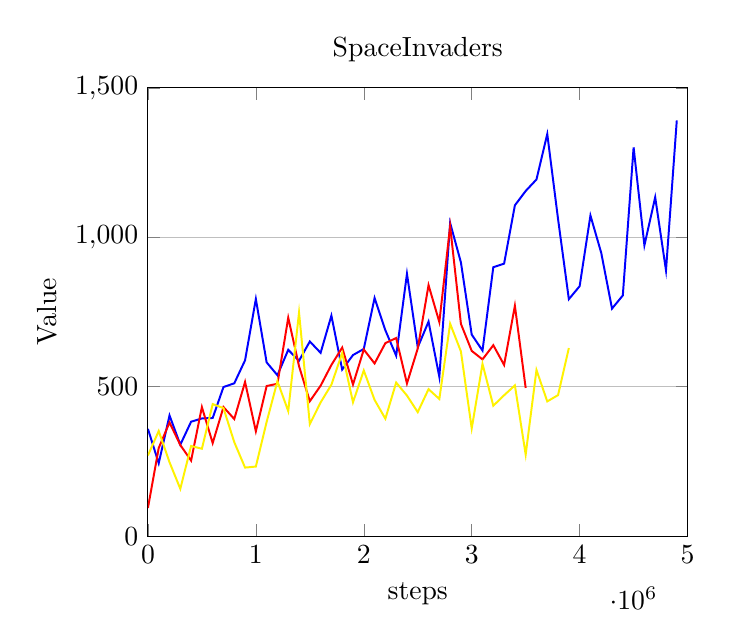
\begin{tikzpicture}

\begin{axis}[%
title=SpaceInvaders,
%width=10in,
%height=5in,
%at={(2.596in,2.358in)},
% scale only axis,
xmin=0,
xmax=5000000,
xlabel style={font=\color{white!15!black}},
xlabel={steps},
xlabel near ticks,
ymin=0,
ymax=1500,
ylabel style={font=\color{white!15!black}},
ylabel={Value},
ylabel near ticks,
ymajorgrids,
% %scale=0.5,
%scale=0.4,
axis background/.style={fill=white},
%legend style={legend cell align=left, align=left, draw=white!15!black}
]
\addplot [color=blue, line width = 0.25mm]
                table[row sep=crcr]{
                  0 359.0\\ 
100000 244.0\\ 
200000 404.0\\ 
300000 306.0\\ 
400000 383.0\\ 
500000 394.0\\ 
600000 395.5\\ 
700000 499.0\\ 
800000 511.5\\ 
900000 588.5\\ 
1000000 793.5\\ 
1100000 581.5\\ 
1200000 538.5\\ 
1300000 623.5\\ 
1400000 587.0\\ 
1500000 651.5\\ 
1600000 613.5\\ 
1700000 738.0\\ 
1800000 557.5\\ 
1900000 606.0\\ 
2000000 626.5\\ 
2100000 797.0\\ 
2200000 689.0\\ 
2300000 604.0\\ 
2400000 878.0\\ 
2500000 632.0\\ 
2600000 718.0\\ 
2700000 533.0\\ 
2800000 1048.0\\ 
2900000 916.0\\ 
3000000 674.5\\ 
3100000 621.0\\ 
3200000 900.0\\ 
3300000 912.0\\ 
3400000 1107.0\\ 
3500000 1155.0\\ 
3600000 1193.5\\ 
3700000 1345.5\\ 
3800000 1061.0\\ 
3900000 793.0\\ 
4000000 836.5\\ 
4100000 1073.0\\ 
4200000 948.0\\ 
4300000 761.5\\ 
4400000 805.5\\ 
4500000 1301.0\\ 
4600000 973.0\\ 
4700000 1134.0\\ 
4800000 889.5\\ 
4900000 1391.0\\ 
};
\addplot [color=red, line width = 0.25mm]
                table[row sep=crcr]{
                  0 94.5\\ 
100000 295.0\\ 
200000 380.5\\ 
300000 305.0\\ 
400000 253.0\\ 
500000 432.0\\ 
600000 311.5\\ 
700000 432.0\\ 
800000 392.0\\ 
900000 516.0\\ 
1000000 351.0\\ 
1100000 502.5\\ 
1200000 510.0\\ 
1300000 731.0\\ 
1400000 569.0\\ 
1500000 451.5\\ 
1600000 503.5\\ 
1700000 573.0\\ 
1800000 631.0\\ 
1900000 507.5\\ 
2000000 624.5\\ 
2100000 578.0\\ 
2200000 646.0\\ 
2300000 663.0\\ 
2400000 511.0\\ 
2500000 628.0\\ 
2600000 840.0\\ 
2700000 716.5\\ 
2800000 1037.0\\ 
2900000 710.5\\ 
3000000 620.0\\ 
3100000 591.5\\ 
3200000 639.0\\ 
3300000 573.0\\ 
3400000 771.0\\ 
3500000 496.0\\ 
};
\addplot [color=yellow, line width = 0.25mm]
                table[row sep=crcr]{
                  0 270.0\\ 
100000 352.0\\ 
200000 247.5\\ 
300000 158.5\\ 
400000 302.0\\ 
500000 292.5\\ 
600000 442.0\\ 
700000 428.5\\ 
800000 314.5\\ 
900000 229.5\\ 
1000000 233.0\\ 
1100000 382.5\\ 
1200000 518.5\\ 
1300000 418.5\\ 
1400000 748.5\\ 
1500000 375.0\\ 
1600000 447.5\\ 
1700000 507.0\\ 
1800000 613.0\\ 
1900000 448.0\\ 
2000000 554.5\\ 
2100000 456.0\\ 
2200000 393.0\\ 
2300000 514.0\\ 
2400000 470.5\\ 
2500000 415.0\\ 
2600000 492.0\\ 
2700000 459.0\\ 
2800000 711.0\\ 
2900000 618.0\\ 
3000000 360.5\\ 
3100000 576.5\\ 
3200000 436.5\\ 
3300000 471.5\\ 
3400000 504.5\\ 
3500000 273.0\\ 
3600000 556.0\\ 
3700000 451.0\\ 
3800000 472.0\\ 
3900000 629.5\\ 
};
\end{axis}
\end{tikzpicture}}} \\
    \ref{named}
\end{figure}
\end{frame}
%  \caption{The graphs of potential efficiency gains. As can be observed from the graphs,
%  if training is started using an encoder which was already trained using
%only reinforcement learning better results are achieved more quickly. Of course, this does not
%encompass all potential benefits --- unsupervised learning could make the problem easier overall
%and thereby allow for both even faster learning and higher final scores.}



\begin{frame}[plain]
		\centering
		\underline{Effect of different encoder sizes on RL}
		\vspace{-1cm}
\begin{figure}[!t]
  \captionsetup[subfloat]{position=top,labelformat=empty}
  \centering
    \subfloat[]{  \resizebox{0.4\textwidth}{!}{
%\definecolor{blue}{RGB}{76,100,135}
%\definecolor{red}{RGB}{153,0,0}
%\definecolor{yellow}{RGB}{227,178,60}
%\definecolor{mycolor1}{rgb}{0.00000,0.44700,0.74100}%
%\definecolor{mycolor2}{rgb}{0.85000,0.32500,0.09800}%
%\definecolor{mycolor3}{rgb}{0.92900,0.69400,0.12500}%
%
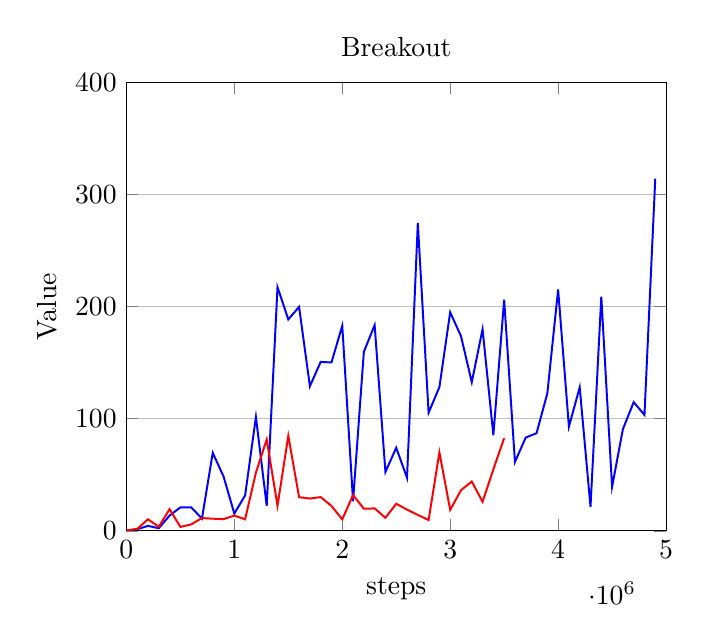
\begin{tikzpicture}

\begin{axis}[%
legend entries={rl-only-small-net,L2-reg,parallel-fs-50-no-aug}, 
legend columns=2,
title=Breakout,
legend to name=named,
legend style={legend cell align=left},
%%width=10in,
%%height=5in,
%%at={(2.596in,2.358in)},
% scale only axis,
xmin=0,
xmax=5000000,
xlabel style={font=\color{white!15!black}},
xlabel={steps},
xlabel near ticks,
ymin=0,
ymax=400,
ylabel style={font=\color{white!15!black}},
ylabel={Value},
ylabel near ticks,
ymajorgrids,
% %scale=0.5,
%%scale=0.4,
axis background/.style={fill=white},
%legend columns=2,
%legend=south outside
]
\addplot [color=blue, line width = 0.25mm]
                table[row sep=crcr]{
                  0 0.20000000298023224\\ 
100000 1.399999976158142\\ 
200000 4.400000095367432\\ 
300000 2.299999952316284\\ 
400000 13.600000381469727\\ 
500000 20.899999618530273\\ 
600000 21.0\\ 
700000 10.899999618530273\\ 
800000 69.5999984741211\\ 
900000 48.5\\ 
1000000 15.399999618530273\\ 
1100000 31.600000381469727\\ 
1200000 101.5999984741211\\ 
1300000 22.399999618530273\\ 
1400000 217.39999389648438\\ 
1500000 188.60000610351562\\ 
1600000 199.8000030517578\\ 
1700000 129.0\\ 
1800000 150.6999969482422\\ 
1900000 150.1999969482422\\ 
2000000 183.0\\ 
2100000 26.399999618530273\\ 
2200000 159.6999969482422\\ 
2300000 183.5\\ 
2400000 52.5\\ 
2500000 74.0999984741211\\ 
2600000 47.29999923706055\\ 
2700000 274.6000061035156\\ 
2800000 105.4000015258789\\ 
2900000 128.1999969482422\\ 
3000000 195.0\\ 
3100000 173.6999969482422\\ 
3200000 132.60000610351562\\ 
3300000 179.89999389648438\\ 
3400000 85.19999694824219\\ 
3500000 206.1999969482422\\ 
3600000 61.5\\ 
3700000 83.19999694824219\\ 
3800000 87.0999984741211\\ 
3900000 122.5999984741211\\ 
4000000 215.3000030517578\\ 
4100000 92.9000015258789\\ 
4200000 128.0\\ 
4300000 21.399999618530273\\ 
4400000 208.89999389648438\\ 
4500000 39.20000076293945\\ 
4600000 90.5999984741211\\ 
4700000 114.80000305175781\\ 
4800000 103.4000015258789\\ 
4900000 314.20001220703125\\ 
};
\addplot [color=red, line width = 0.25mm]
                table[row sep=crcr]{
                  0 0.4000000059604645\\ 
100000 1.7000000476837158\\ 
200000 10.300000190734863\\ 
300000 3.5999999046325684\\ 
400000 19.299999237060547\\ 
500000 3.5\\ 
600000 5.699999809265137\\ 
700000 11.399999618530273\\ 
800000 10.800000190734863\\ 
900000 10.399999618530273\\ 
1000000 13.600000381469727\\ 
1100000 10.300000190734863\\ 
1200000 51.900001525878906\\ 
1300000 81.5\\ 
1400000 22.299999237060547\\ 
1500000 84.69999694824219\\ 
1600000 30.0\\ 
1700000 28.799999237060547\\ 
1800000 30.100000381469727\\ 
1900000 22.200000762939453\\ 
2000000 10.199999809265137\\ 
2100000 31.899999618530273\\ 
2200000 19.700000762939453\\ 
2300000 20.0\\ 
2400000 11.600000381469727\\ 
2500000 24.200000762939453\\ 
2600000 18.899999618530273\\ 
2700000 14.199999809265137\\ 
2800000 9.600000381469727\\ 
2900000 70.0\\ 
3000000 18.700000762939453\\ 
3100000 36.20000076293945\\ 
3200000 44.0\\ 
3300000 25.899999618530273\\ 
3400000 54.900001525878906\\ 
3500000 82.69999694824219\\ 
};
\addplot [color=yellow, line width = 0.25mm]
                table[row sep=crcr]{
                  0 0.800000011920929\\ 
};
\end{axis}
\end{tikzpicture}}}
    \subfloat[]{  \resizebox{0.4\textwidth}{!}{
%\definecolor{blue}{RGB}{76,100,135}
%\definecolor{red}{RGB}{153,0,0}
%\definecolor{yellow}{RGB}{227,178,60}
%\definecolor{mycolor1}{rgb}{0.00000,0.44700,0.74100}%
%\definecolor{mycolor2}{rgb}{0.85000,0.32500,0.09800}%
%\definecolor{mycolor3}{rgb}{0.92900,0.69400,0.12500}%
%
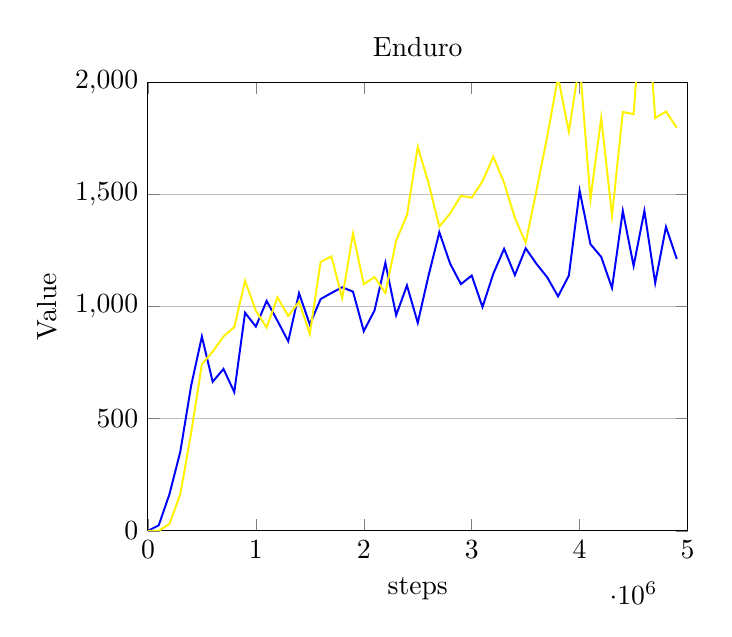
\begin{tikzpicture}

\begin{axis}[%
title=Enduro,
% %width=4.634in,
%%width=10in,
%%height=5in,
%at={(2.596in,2.358in)},
% scale only axis,
xmin=0,
xmax=5000000,
xlabel style={font=\color{white!15!black}},
xlabel={steps},
xlabel near ticks,
ymin=0,
ymax=2000,
ylabel style={font=\color{white!15!black}},
ylabel={Value},
ylabel near ticks,
ymajorgrids,
% %scale=0.5,
%scale=0.4,
axis background/.style={fill=white},
%legend style={legend cell align=left, align=left, draw=white!15!black}
]
\addplot [color=blue, line width = 0.25mm]
                table[row sep=crcr]{
                  0 0.0\\ 
100000 24.299999237060547\\ 
200000 164.3000030517578\\ 
300000 353.0\\ 
400000 646.4000244140625\\ 
500000 866.7000122070312\\ 
600000 664.7000122070312\\ 
700000 722.2000122070312\\ 
800000 618.9000244140625\\ 
900000 972.7999877929688\\ 
1000000 910.9000244140625\\ 
1100000 1025.699951171875\\ 
1200000 937.0\\ 
1300000 845.5999755859375\\ 
1400000 1059.9000244140625\\ 
1500000 920.2999877929688\\ 
1600000 1033.800048828125\\ 
1700000 1061.0\\ 
1800000 1086.5999755859375\\ 
1900000 1066.9000244140625\\ 
2000000 890.9000244140625\\ 
2100000 983.5\\ 
2200000 1195.300048828125\\ 
2300000 962.0\\ 
2400000 1094.800048828125\\ 
2500000 928.0\\ 
2600000 1138.5999755859375\\ 
2700000 1332.300048828125\\ 
2800000 1191.800048828125\\ 
2900000 1100.5999755859375\\ 
3000000 1138.800048828125\\ 
3100000 998.2999877929688\\ 
3200000 1146.800048828125\\ 
3300000 1258.0999755859375\\ 
3400000 1141.0\\ 
3500000 1260.300048828125\\ 
3600000 1190.800048828125\\ 
3700000 1130.5999755859375\\ 
3800000 1046.0999755859375\\ 
3900000 1138.4000244140625\\ 
4000000 1517.5\\ 
4100000 1278.9000244140625\\ 
4200000 1221.699951171875\\ 
4300000 1083.199951171875\\ 
4400000 1426.9000244140625\\ 
4500000 1181.5999755859375\\ 
4600000 1427.199951171875\\ 
4700000 1105.800048828125\\ 
4800000 1355.800048828125\\ 
4900000 1212.9000244140625\\ 
};
\addplot [color=red, line width = 0.25mm]
                table[row sep=crcr]{
                  0 0.0\\ 
};
\addplot [color=yellow, line width = 0.25mm]
                table[row sep=crcr]{
                  0 0.0\\ 
100000 0.0\\ 
200000 30.700000762939453\\ 
300000 163.6999969482422\\ 
400000 435.79998779296875\\ 
500000 743.2000122070312\\ 
600000 799.2000122070312\\ 
700000 867.0\\ 
800000 908.4000244140625\\ 
900000 1115.300048828125\\ 
1000000 981.4000244140625\\ 
1100000 906.9000244140625\\ 
1200000 1041.5999755859375\\ 
1300000 958.5999755859375\\ 
1400000 1021.9000244140625\\ 
1500000 877.7000122070312\\ 
1600000 1199.4000244140625\\ 
1700000 1224.0\\ 
1800000 1038.199951171875\\ 
1900000 1326.0999755859375\\ 
2000000 1100.0\\ 
2100000 1132.0999755859375\\ 
2200000 1060.9000244140625\\ 
2300000 1294.300048828125\\ 
2400000 1407.699951171875\\ 
2500000 1712.5\\ 
2600000 1551.5\\ 
2700000 1357.0\\ 
2800000 1415.800048828125\\ 
2900000 1494.5\\ 
3000000 1486.0\\ 
3100000 1559.699951171875\\ 
3200000 1668.5\\ 
3300000 1552.800048828125\\ 
3400000 1395.800048828125\\ 
3500000 1284.9000244140625\\ 
3600000 1518.0\\ 
3700000 1759.5999755859375\\ 
3800000 2024.9000244140625\\ 
3900000 1780.0999755859375\\ 
4000000 2090.5\\ 
4100000 1479.0999755859375\\ 
4200000 1841.699951171875\\ 
4300000 1405.5999755859375\\ 
4400000 1868.300048828125\\ 
4500000 1858.699951171875\\ 
4600000 2527.0\\ 
4700000 1841.0\\ 
4800000 1870.800048828125\\ 
4900000 1797.9000244140625\\ 
};
\end{axis}
\end{tikzpicture}}}\\
  \vspace{-1cm}
    \subfloat[]{  \resizebox{0.4\textwidth}{!}{
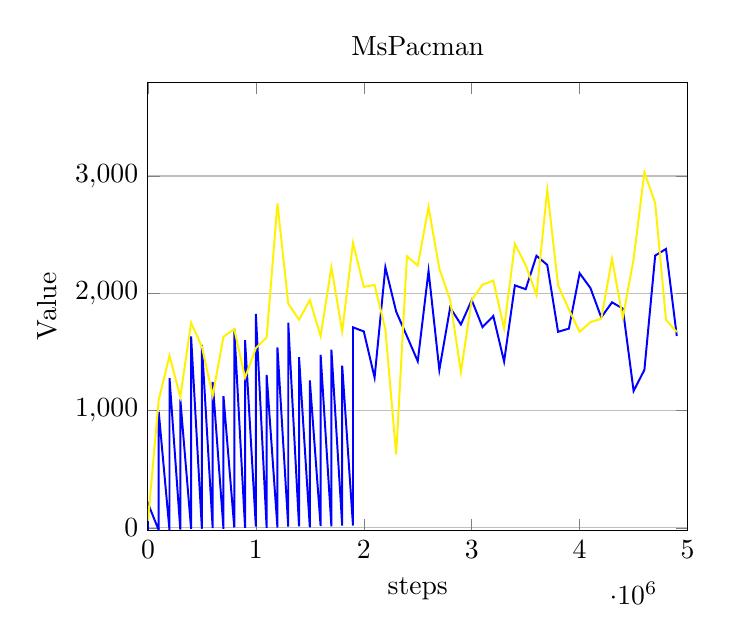
\begin{tikzpicture}

\begin{axis}[%
title=MsPacman,
% %width=4.634in,
%width=10in,
%height=5in,
%at={(2.596in,2.358in)},
% scale only axis,
xmin=0,
xmax=5000000,
xlabel style={font=\color{white!15!black}},
xlabel={steps},
xlabel near ticks,
ymin=-22,
ymax=3800,
ylabel style={font=\color{white!15!black}},
ylabel={Value},
ylabel near ticks,
ymajorgrids,
% %scale=0.5,
%scale=0.4,
axis background/.style={fill=white},
%legend style={legend cell align=left, align=left, draw=white!15!black}
]
\addplot [color=blue, line width = 0.25mm]
                table[row sep=crcr]{
                  0 -21.0\\ 
0 210.0\\ 
100000 -19.799999237060547\\ 
100000 990.0\\ 
200000 -20.700000762939453\\ 
200000 1277.0\\ 
300000 -15.0\\ 
300000 1096.0\\ 
400000 -7.0\\ 
400000 1632.0\\ 
500000 -6.900000095367432\\ 
500000 1561.0\\ 
600000 -1.899999976158142\\ 
600000 1245.0\\ 
700000 -7.599999904632568\\ 
700000 1123.0\\ 
800000 4.0\\ 
800000 1696.0\\ 
900000 1.5\\ 
900000 1600.0\\ 
1000000 11.300000190734863\\ 
1000000 1824.0\\ 
1100000 1.2000000476837158\\ 
1100000 1304.0\\ 
1200000 3.700000047683716\\ 
1200000 1538.0\\ 
1300000 11.5\\ 
1300000 1750.0\\ 
1400000 13.600000381469727\\ 
1400000 1456.0\\ 
1500000 5.699999809265137\\ 
1500000 1258.0\\ 
1600000 15.600000381469727\\ 
1600000 1476.0\\ 
1700000 13.5\\ 
1700000 1519.0\\ 
1800000 19.299999237060547\\ 
1800000 1383.0\\ 
1900000 20.799999237060547\\ 
1900000 1710.0\\ 
2000000 1675.0\\ 
2100000 1282.0\\ 
2200000 2222.0\\ 
2300000 1844.0\\ 
2400000 1634.0\\ 
2500000 1421.0\\ 
2600000 2191.0\\ 
2700000 1347.0\\ 
2800000 1878.0\\ 
2900000 1735.0\\ 
3000000 1942.0\\ 
3100000 1712.0\\ 
3200000 1806.0\\ 
3300000 1419.0\\ 
3400000 2068.0\\ 
3500000 2035.0\\ 
3600000 2320.0\\ 
3700000 2242.0\\ 
3800000 1672.0\\ 
3900000 1699.0\\ 
4000000 2171.0\\ 
4100000 2045.0\\ 
4200000 1795.0\\ 
4300000 1923.0\\ 
4400000 1870.0\\ 
4500000 1167.0\\ 
4600000 1348.0\\ 
4700000 2322.0\\ 
4800000 2378.0\\ 
4900000 1636.0\\ 
};
\addplot [color=red, line width = 0.25mm]
                table[row sep=crcr]{
                  0 0.0\\ 
};
\addplot [color=yellow, line width = 0.25mm]
                table[row sep=crcr]{
                  0 60.0\\ 
100000 1090.0\\ 
200000 1469.0\\ 
300000 1117.0\\ 
400000 1749.0\\ 
500000 1545.0\\ 
600000 1128.0\\ 
700000 1630.0\\ 
800000 1695.0\\ 
900000 1281.0\\ 
1000000 1532.0\\ 
1100000 1625.0\\ 
1200000 2767.0\\ 
1300000 1912.0\\ 
1400000 1775.0\\ 
1500000 1942.0\\ 
1600000 1636.0\\ 
1700000 2222.0\\ 
1800000 1676.0\\ 
1900000 2430.0\\ 
2000000 2055.0\\ 
2100000 2072.0\\ 
2200000 1693.0\\ 
2300000 625.0\\ 
2400000 2317.0\\ 
2500000 2236.0\\ 
2600000 2736.0\\ 
2700000 2209.0\\ 
2800000 1944.0\\ 
2900000 1329.0\\ 
3000000 1944.0\\ 
3100000 2074.0\\ 
3200000 2109.0\\ 
3300000 1701.0\\ 
3400000 2421.0\\ 
3500000 2240.0\\ 
3600000 1986.0\\ 
3700000 2883.0\\ 
3800000 2069.0\\ 
3900000 1863.0\\ 
4000000 1672.0\\ 
4100000 1754.0\\ 
4200000 1783.0\\ 
4300000 2293.0\\ 
4400000 1791.0\\ 
4500000 2293.0\\ 
4600000 3033.0\\ 
4700000 2768.0\\ 
4800000 1774.0\\ 
4900000 1670.0\\ 
};
\end{axis}
\end{tikzpicture}}}
    \subfloat[]{  \resizebox{0.4\textwidth}{!}{
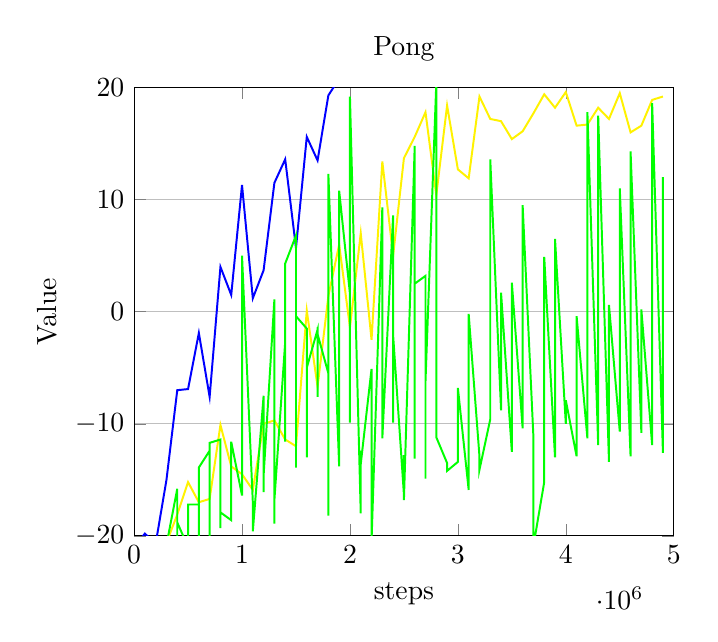
\begin{tikzpicture}

\begin{axis}[%
title=Pong,
% %width=4.634in,
%width=10in,
%height=5in,
%at={(2.596in,2.358in)},
% scale only axis,
xmin=0,
xmax=5000000,
xlabel style={font=\color{white!15!black}},
xlabel={steps},
xlabel near ticks,
ymin=-20,
ymax=20,
ylabel style={font=\color{white!15!black}},
ylabel={Value},
ylabel near ticks,
ymajorgrids,
% %scale=0.5,
%scale=0.4,
axis background/.style={fill=white},
%legend style={legend cell align=left, align=left, draw=white!15!black}
]
\addplot [color=blue, line width = 0.25mm]
                table[row sep=crcr]{
                  0 -21.0\\ 
100000 -19.799999237060547\\ 
200000 -20.700000762939453\\ 
300000 -15.0\\ 
400000 -7.0\\ 
500000 -6.900000095367432\\ 
600000 -1.899999976158142\\ 
700000 -7.599999904632568\\ 
800000 4.0\\ 
900000 1.5\\ 
1000000 11.300000190734863\\ 
1100000 1.2000000476837158\\ 
1200000 3.700000047683716\\ 
1300000 11.5\\ 
1400000 13.600000381469727\\ 
1500000 5.699999809265137\\ 
1600000 15.600000381469727\\ 
1700000 13.5\\ 
1800000 19.299999237060547\\ 
1900000 20.799999237060547\\ 
};
\addplot [color=red, line width = 0.25mm]
                table[row sep=crcr]{
                  0 0.0\\ 
};
\addplot [color=yellow, line width = 0.25mm]
                table[row sep=crcr]{
                  0 -21.0\\ 
0 -21.0\\ 
0 -21.0\\ 
100000 -21.0\\ 
200000 -20.299999237060547\\ 
300000 -20.600000381469727\\ 
400000 -18.100000381469727\\ 
500000 -15.199999809265137\\ 
600000 -17.0\\ 
700000 -16.700000762939453\\ 
800000 -10.100000381469727\\ 
900000 -13.800000190734863\\ 
1000000 -14.5\\ 
1100000 -15.899999618530273\\ 
1200000 -10.0\\ 
1300000 -9.699999809265137\\ 
1400000 -11.399999618530273\\ 
1500000 -12.0\\ 
1600000 0.10000000149011612\\ 
1700000 -6.699999809265137\\ 
1800000 1.399999976158142\\ 
1900000 6.0\\ 
2000000 -1.399999976158142\\ 
2100000 7.0\\ 
2200000 -2.5\\ 
2300000 13.399999618530273\\ 
2400000 5.0\\ 
2500000 13.699999809265137\\ 
2600000 15.600000381469727\\ 
2700000 17.799999237060547\\ 
2800000 10.399999618530273\\ 
2900000 18.399999618530273\\ 
3000000 12.699999809265137\\ 
3100000 11.899999618530273\\ 
3200000 19.200000762939453\\ 
3300000 17.200000762939453\\ 
3400000 17.0\\ 
3500000 15.399999618530273\\ 
3600000 16.100000381469727\\ 
3700000 17.700000762939453\\ 
3800000 19.399999618530273\\ 
3900000 18.200000762939453\\ 
4000000 19.600000381469727\\ 
4100000 16.600000381469727\\ 
4200000 16.700000762939453\\ 
4300000 18.200000762939453\\ 
4400000 17.200000762939453\\ 
4500000 19.5\\ 
4600000 16.0\\ 
4700000 16.600000381469727\\ 
4800000 18.899999618530273\\ 
4900000 19.200000762939453\\ 
};
\addplot [color=green, line width = 0.25mm]
                table[row sep=crcr]{
                  0 -21.0\\ 
0 -21.0\\ 
0 -21.0\\ 
0 -21.0\\ 
100000 -21.0\\ 
100000 -20.600000381469727\\ 
100000 -21.0\\ 
200000 -20.399999618530273\\ 
200000 -21.0\\ 
200000 -20.799999237060547\\ 
300000 -20.600000381469727\\ 
300000 -20.799999237060547\\ 
300000 -20.799999237060547\\ 
400000 -15.800000190734863\\ 
400000 -20.399999618530273\\ 
400000 -18.799999237060547\\ 
500000 -21.0\\ 
500000 -21.0\\ 
500000 -17.200000762939453\\ 
600000 -17.200000762939453\\ 
600000 -20.600000381469727\\ 
600000 -13.899999618530273\\ 
700000 -12.399999618530273\\ 
700000 -20.100000381469727\\ 
700000 -11.699999809265137\\ 
800000 -11.399999618530273\\ 
800000 -19.299999237060547\\ 
800000 -17.899999618530273\\ 
900000 -18.600000381469727\\ 
900000 -15.699999809265137\\ 
900000 -11.600000381469727\\ 
1000000 -16.399999618530273\\ 
1000000 -16.0\\ 
1000000 5.0\\ 
1100000 -17.0\\ 
1100000 -17.5\\ 
1100000 -19.600000381469727\\ 
1200000 -7.5\\ 
1200000 -16.100000381469727\\ 
1200000 -14.600000381469727\\ 
1300000 1.100000023841858\\ 
1300000 -18.899999618530273\\ 
1300000 -16.799999237060547\\ 
1400000 -2.700000047683716\\ 
1400000 -11.600000381469727\\ 
1400000 4.300000190734863\\ 
1500000 6.800000190734863\\ 
1500000 -13.899999618530273\\ 
1500000 -0.4000000059604645\\ 
1600000 -1.5\\ 
1600000 -13.0\\ 
1600000 -5.0\\ 
1700000 -1.600000023841858\\ 
1700000 -7.599999904632568\\ 
1700000 -2.0\\ 
1800000 -5.5\\ 
1800000 -18.200000762939453\\ 
1800000 12.300000190734863\\ 
1900000 -13.800000190734863\\ 
1900000 -10.0\\ 
1900000 10.800000190734863\\ 
2000000 1.600000023841858\\ 
2000000 -9.899999618530273\\ 
2000000 19.200000762939453\\ 
2100000 -18.0\\ 
2100000 -12.399999618530273\\ 
2100000 -13.600000381469727\\ 
2200000 -5.099999904632568\\ 
2200000 -13.899999618530273\\ 
2200000 -20.5\\ 
2300000 9.300000190734863\\ 
2300000 -8.199999809265137\\ 
2300000 -11.300000190734863\\ 
2400000 8.600000381469727\\ 
2400000 -9.899999618530273\\ 
2400000 -2.0999999046325684\\ 
2500000 -16.299999237060547\\ 
2500000 -12.800000190734863\\ 
2500000 -16.799999237060547\\ 
2600000 14.800000190734863\\ 
2600000 -13.100000381469727\\ 
2600000 2.5\\ 
2700000 3.200000047683716\\ 
2700000 -14.899999618530273\\ 
2700000 -6.199999809265137\\ 
2800000 20.399999618530273\\ 
2800000 -9.800000190734863\\ 
2800000 -11.199999809265137\\ 
2900000 -13.5\\ 
2900000 -14.199999809265137\\ 
3000000 -13.399999618530273\\ 
3000000 -6.800000190734863\\ 
3100000 -15.899999618530273\\ 
3100000 -0.20000000298023224\\ 
3200000 -12.899999618530273\\ 
3200000 -14.100000381469727\\ 
3300000 -9.600000381469727\\ 
3300000 13.600000381469727\\ 
3400000 -8.800000190734863\\ 
3400000 1.7000000476837158\\ 
3500000 -12.5\\ 
3500000 2.5999999046325684\\ 
3600000 -10.399999618530273\\ 
3600000 9.5\\ 
3700000 -11.199999809265137\\ 
3700000 -20.899999618530273\\ 
3800000 -15.199999809265137\\ 
3800000 4.900000095367432\\ 
3900000 -13.0\\ 
3900000 6.5\\ 
4000000 -10.0\\ 
4000000 -7.900000095367432\\ 
4100000 -12.899999618530273\\ 
4100000 -0.4000000059604645\\ 
4200000 -11.300000190734863\\ 
4200000 17.799999237060547\\ 
4300000 -11.899999618530273\\ 
4300000 17.5\\ 
4400000 -13.399999618530273\\ 
4400000 0.6000000238418579\\ 
4500000 -10.699999809265137\\ 
4500000 11.0\\ 
4600000 -12.899999618530273\\ 
4600000 14.300000190734863\\ 
4700000 -10.800000190734863\\ 
4700000 0.20000000298023224\\ 
4800000 -11.899999618530273\\ 
4800000 18.600000381469727\\ 
4900000 -12.600000381469727\\ 
4900000 12.0\\ 
};
\end{axis}
\end{tikzpicture}}}\\
%  \vspace{-1cm}
    \ref{named}
%  \label{fig:rl-only-vs-pretrained}
\end{figure}
\end{frame}


\begin{frame}[plain]
%{Effectiveness of pretraining --- continued}
		\centering
		\underline{Effect of different encoder sizes on RL --- continued}
		\vspace{-1cm}
\begin{figure}[!t]
  \captionsetup[subfloat]{position=top,labelformat=empty}
  \centering
    \subfloat[]{  \resizebox{0.4\textwidth}{!}{
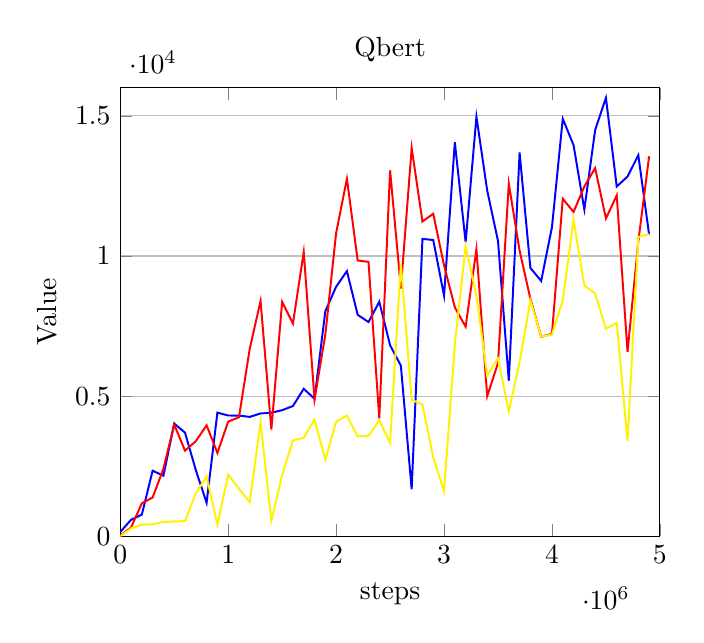
\begin{tikzpicture}

\begin{axis}[%
title=Qbert,
% %width=4.634in,
%width=10in,
%height=5in,
%at={(2.596in,2.358in)},
% scale only axis,
xmin=0,
xmax=5000000,
xlabel style={font=\color{white!15!black}},
xlabel={steps},
xlabel near ticks,
ymin=0,
ymax=16000,
ylabel style={font=\color{white!15!black}},
ylabel={Value},
ylabel near ticks,
ymajorgrids,
% %scale=0.5,
%scale=0.4,
axis background/.style={fill=white},
%legend style={legend cell align=left, align=left, draw=white!15!black}
]
\addplot [color=blue, line width = 0.25mm]
                table[row sep=crcr]{
                  0 150.0\\ 
100000 585.0\\ 
200000 772.5\\ 
300000 2337.5\\ 
400000 2157.5\\ 
500000 4022.5\\ 
600000 3695.0\\ 
700000 2362.5\\ 
800000 1192.5\\ 
900000 4410.0\\ 
1000000 4307.5\\ 
1100000 4305.0\\ 
1200000 4257.5\\ 
1300000 4380.0\\ 
1400000 4407.5\\ 
1500000 4497.5\\ 
1600000 4645.0\\ 
1700000 5260.0\\ 
1800000 4905.0\\ 
1900000 8030.0\\ 
2000000 8902.5\\ 
2100000 9460.0\\ 
2200000 7900.0\\ 
2300000 7642.5\\ 
2400000 8367.5\\ 
2500000 6815.0\\ 
2600000 6085.0\\ 
2700000 1677.5\\ 
2800000 10610.0\\ 
2900000 10570.0\\ 
3000000 8585.0\\ 
3100000 14057.5\\ 
3200000 10490.0\\ 
3300000 14970.0\\ 
3400000 12332.5\\ 
3500000 10537.5\\ 
3600000 5550.0\\ 
3700000 13692.5\\ 
3800000 9572.5\\ 
3900000 9110.0\\ 
4000000 11030.0\\ 
4100000 14897.5\\ 
4200000 13955.0\\ 
4300000 11660.0\\ 
4400000 14495.0\\ 
4500000 15645.0\\ 
4600000 12480.0\\ 
4700000 12835.0\\ 
4800000 13597.5\\ 
4900000 10762.5\\ 
};
\addplot [color=red, line width = 0.25mm]
                table[row sep=crcr]{
                  0 22.5\\ 
100000 310.0\\ 
200000 1172.5\\ 
300000 1382.5\\ 
400000 2410.0\\ 
500000 3982.5\\ 
600000 3052.5\\ 
700000 3390.0\\ 
800000 3957.5\\ 
900000 2970.0\\ 
1000000 4090.0\\ 
1100000 4245.0\\ 
1200000 6697.5\\ 
1300000 8395.0\\ 
1400000 3807.5\\ 
1500000 8360.0\\ 
1600000 7590.0\\ 
1700000 10142.5\\ 
1800000 4877.5\\ 
1900000 7190.0\\ 
2000000 10817.5\\ 
2100000 12755.0\\ 
2200000 9840.0\\ 
2300000 9790.0\\ 
2400000 4202.5\\ 
2500000 13057.5\\ 
2600000 8842.5\\ 
2700000 13852.5\\ 
2800000 11230.0\\ 
2900000 11507.5\\ 
3000000 9665.0\\ 
3100000 8167.5\\ 
3200000 7475.0\\ 
3300000 10242.5\\ 
3400000 4997.5\\ 
3500000 6180.0\\ 
3600000 12582.5\\ 
3700000 10190.0\\ 
3800000 8475.0\\ 
3900000 7115.0\\ 
4000000 7222.5\\ 
4100000 12042.5\\ 
4200000 11572.5\\ 
4300000 12480.0\\ 
4400000 13137.5\\ 
4500000 11337.5\\ 
4600000 12165.0\\ 
4700000 6580.0\\ 
4800000 10517.5\\ 
4900000 13560.0\\ 
};
\addplot [color=yellow, line width = 0.25mm]
                table[row sep=crcr]{
                  0 0.0\\ 
100000 280.0\\ 
200000 415.0\\ 
300000 425.0\\ 
400000 507.5\\ 
500000 525.0\\ 
600000 537.5\\ 
700000 1525.0\\ 
800000 2137.5\\ 
900000 407.5\\ 
1000000 2195.0\\ 
1100000 1690.0\\ 
1200000 1215.0\\ 
1300000 4077.5\\ 
1400000 550.0\\ 
1500000 2185.0\\ 
1600000 3417.5\\ 
1700000 3512.5\\ 
1800000 4165.0\\ 
1900000 2730.0\\ 
2000000 4090.0\\ 
2100000 4305.0\\ 
2200000 3557.5\\ 
2300000 3585.0\\ 
2400000 4137.5\\ 
2500000 3335.0\\ 
2600000 9722.5\\ 
2700000 4865.0\\ 
2800000 4700.0\\ 
2900000 2812.5\\ 
3000000 1605.0\\ 
3100000 6847.5\\ 
3200000 10342.5\\ 
3300000 8590.0\\ 
3400000 5732.5\\ 
3500000 6345.0\\ 
3600000 4447.5\\ 
3700000 6217.5\\ 
3800000 8415.0\\ 
3900000 7120.0\\ 
4000000 7195.0\\ 
4100000 8415.0\\ 
4200000 11307.5\\ 
4300000 8942.5\\ 
4400000 8662.5\\ 
4500000 7402.5\\ 
4600000 7612.5\\ 
4700000 3395.0\\ 
4800000 10680.0\\ 
4900000 10780.0\\ 
};
\end{axis}
\end{tikzpicture}}}
    \subfloat[]{  \resizebox{0.4\textwidth}{!}{
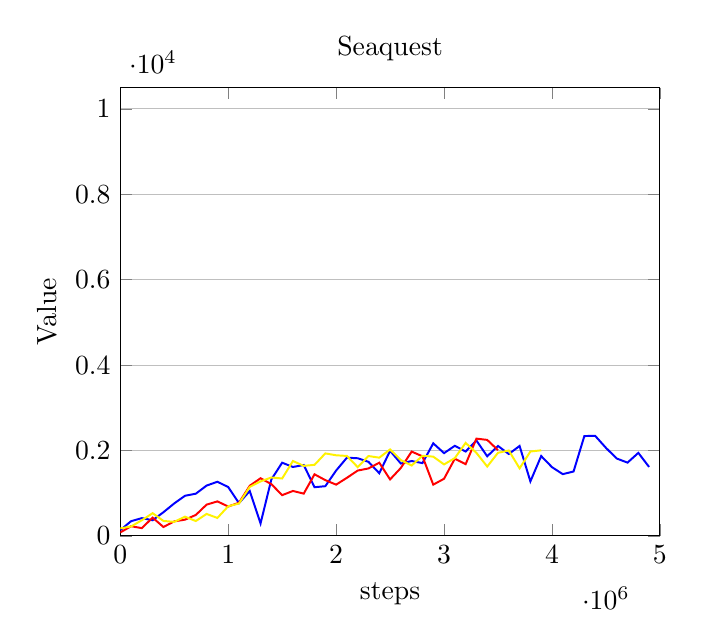
\begin{tikzpicture}

\begin{axis}[%
title=Seaquest,
% %width=4.634in,
%width=10in,
%height=5in,
%at={(2.596in,2.358in)},
% scale only axis,
xmin=0,
xmax=5000000,
xlabel style={font=\color{white!15!black}},
xlabel={steps},
xlabel near ticks,
ymin=0,
ymax=10500,
ylabel style={font=\color{white!15!black}},
ylabel={Value},
ylabel near ticks,
ymajorgrids,
% %scale=0.5,
%scale=0.4,
axis background/.style={fill=white},
%legend style={legend cell align=left, align=left, draw=white!15!black}
]
\addplot [color=blue, line width = 0.25mm]
                table[row sep=crcr]{
                  0 134.0\\ 
100000 344.0\\ 
200000 416.0\\ 
300000 366.0\\ 
400000 554.0\\ 
500000 760.0\\ 
600000 940.0\\ 
700000 988.0\\ 
800000 1178.0\\ 
900000 1268.0\\ 
1000000 1144.0\\ 
1100000 768.0\\ 
1200000 1052.0\\ 
1300000 292.0\\ 
1400000 1322.0\\ 
1500000 1714.0\\ 
1600000 1614.0\\ 
1700000 1660.0\\ 
1800000 1140.0\\ 
1900000 1164.0\\ 
2000000 1530.0\\ 
2100000 1832.0\\ 
2200000 1818.0\\ 
2300000 1734.0\\ 
2400000 1468.0\\ 
2500000 1992.0\\ 
2600000 1694.0\\ 
2700000 1754.0\\ 
2800000 1704.0\\ 
2900000 2168.0\\ 
3000000 1938.0\\ 
3100000 2110.0\\ 
3200000 1976.0\\ 
3300000 2234.0\\ 
3400000 1864.0\\ 
3500000 2106.0\\ 
3600000 1918.0\\ 
3700000 2106.0\\ 
3800000 1276.0\\ 
3900000 1870.0\\ 
4000000 1610.0\\ 
4100000 1446.0\\ 
4200000 1508.0\\ 
4300000 2338.0\\ 
4400000 2344.0\\ 
4500000 2062.0\\ 
4600000 1812.0\\ 
4700000 1716.0\\ 
4800000 1944.0\\ 
4900000 1614.0\\ 
};
\addplot [color=red, line width = 0.25mm]
                table[row sep=crcr]{
                  0 80.0\\ 
100000 226.0\\ 
200000 182.0\\ 
300000 428.0\\ 
400000 208.0\\ 
500000 340.0\\ 
600000 380.0\\ 
700000 490.0\\ 
800000 732.0\\ 
900000 808.0\\ 
1000000 688.0\\ 
1100000 776.0\\ 
1200000 1174.0\\ 
1300000 1350.0\\ 
1400000 1212.0\\ 
1500000 954.0\\ 
1600000 1052.0\\ 
1700000 990.0\\ 
1800000 1442.0\\ 
1900000 1306.0\\ 
2000000 1200.0\\ 
2100000 1360.0\\ 
2200000 1530.0\\ 
2300000 1580.0\\ 
2400000 1714.0\\ 
2500000 1322.0\\ 
2600000 1592.0\\ 
2700000 1974.0\\ 
2800000 1864.0\\ 
2900000 1200.0\\ 
3000000 1338.0\\ 
3100000 1808.0\\ 
3200000 1680.0\\ 
3300000 2278.0\\ 
3400000 2248.0\\ 
3500000 2008.0\\ 
};
\addplot [color=yellow, line width = 0.25mm]
                table[row sep=crcr]{
                  0 176.0\\ 
100000 220.0\\ 
200000 366.0\\ 
300000 532.0\\ 
400000 350.0\\ 
500000 328.0\\ 
600000 450.0\\ 
700000 348.0\\ 
800000 514.0\\ 
900000 420.0\\ 
1000000 694.0\\ 
1100000 758.0\\ 
1200000 1148.0\\ 
1300000 1276.0\\ 
1400000 1368.0\\ 
1500000 1344.0\\ 
1600000 1754.0\\ 
1700000 1640.0\\ 
1800000 1664.0\\ 
1900000 1932.0\\ 
2000000 1888.0\\ 
2100000 1872.0\\ 
2200000 1610.0\\ 
2300000 1870.0\\ 
2400000 1832.0\\ 
2500000 2024.0\\ 
2600000 1774.0\\ 
2700000 1648.0\\ 
2800000 1876.0\\ 
2900000 1856.0\\ 
3000000 1674.0\\ 
3100000 1822.0\\ 
3200000 2178.0\\ 
3300000 1944.0\\ 
3400000 1624.0\\ 
3500000 1946.0\\ 
3600000 2000.0\\ 
3700000 1582.0\\ 
3800000 1976.0\\ 
3900000 2004.0\\ 
};
\end{axis}
\end{tikzpicture}}}\\
  \vspace{-1cm}
    \subfloat[]{  \resizebox{0.4\textwidth}{!}{
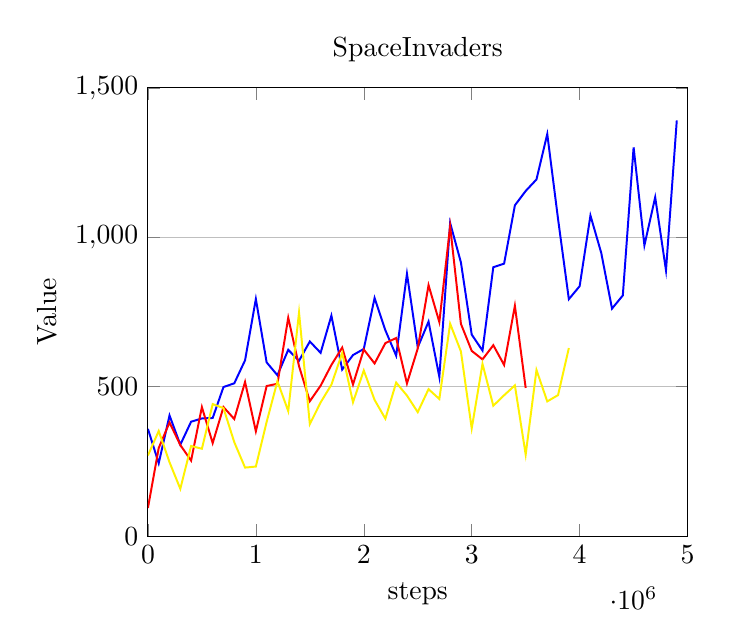
\begin{tikzpicture}

\begin{axis}[%
title=SpaceInvaders,
%width=10in,
%height=5in,
%at={(2.596in,2.358in)},
% scale only axis,
xmin=0,
xmax=5000000,
xlabel style={font=\color{white!15!black}},
xlabel={steps},
xlabel near ticks,
ymin=0,
ymax=1500,
ylabel style={font=\color{white!15!black}},
ylabel={Value},
ylabel near ticks,
ymajorgrids,
% %scale=0.5,
%scale=0.4,
axis background/.style={fill=white},
%legend style={legend cell align=left, align=left, draw=white!15!black}
]
\addplot [color=blue, line width = 0.25mm]
                table[row sep=crcr]{
                  0 359.0\\ 
100000 244.0\\ 
200000 404.0\\ 
300000 306.0\\ 
400000 383.0\\ 
500000 394.0\\ 
600000 395.5\\ 
700000 499.0\\ 
800000 511.5\\ 
900000 588.5\\ 
1000000 793.5\\ 
1100000 581.5\\ 
1200000 538.5\\ 
1300000 623.5\\ 
1400000 587.0\\ 
1500000 651.5\\ 
1600000 613.5\\ 
1700000 738.0\\ 
1800000 557.5\\ 
1900000 606.0\\ 
2000000 626.5\\ 
2100000 797.0\\ 
2200000 689.0\\ 
2300000 604.0\\ 
2400000 878.0\\ 
2500000 632.0\\ 
2600000 718.0\\ 
2700000 533.0\\ 
2800000 1048.0\\ 
2900000 916.0\\ 
3000000 674.5\\ 
3100000 621.0\\ 
3200000 900.0\\ 
3300000 912.0\\ 
3400000 1107.0\\ 
3500000 1155.0\\ 
3600000 1193.5\\ 
3700000 1345.5\\ 
3800000 1061.0\\ 
3900000 793.0\\ 
4000000 836.5\\ 
4100000 1073.0\\ 
4200000 948.0\\ 
4300000 761.5\\ 
4400000 805.5\\ 
4500000 1301.0\\ 
4600000 973.0\\ 
4700000 1134.0\\ 
4800000 889.5\\ 
4900000 1391.0\\ 
};
\addplot [color=red, line width = 0.25mm]
                table[row sep=crcr]{
                  0 94.5\\ 
100000 295.0\\ 
200000 380.5\\ 
300000 305.0\\ 
400000 253.0\\ 
500000 432.0\\ 
600000 311.5\\ 
700000 432.0\\ 
800000 392.0\\ 
900000 516.0\\ 
1000000 351.0\\ 
1100000 502.5\\ 
1200000 510.0\\ 
1300000 731.0\\ 
1400000 569.0\\ 
1500000 451.5\\ 
1600000 503.5\\ 
1700000 573.0\\ 
1800000 631.0\\ 
1900000 507.5\\ 
2000000 624.5\\ 
2100000 578.0\\ 
2200000 646.0\\ 
2300000 663.0\\ 
2400000 511.0\\ 
2500000 628.0\\ 
2600000 840.0\\ 
2700000 716.5\\ 
2800000 1037.0\\ 
2900000 710.5\\ 
3000000 620.0\\ 
3100000 591.5\\ 
3200000 639.0\\ 
3300000 573.0\\ 
3400000 771.0\\ 
3500000 496.0\\ 
};
\addplot [color=yellow, line width = 0.25mm]
                table[row sep=crcr]{
                  0 270.0\\ 
100000 352.0\\ 
200000 247.5\\ 
300000 158.5\\ 
400000 302.0\\ 
500000 292.5\\ 
600000 442.0\\ 
700000 428.5\\ 
800000 314.5\\ 
900000 229.5\\ 
1000000 233.0\\ 
1100000 382.5\\ 
1200000 518.5\\ 
1300000 418.5\\ 
1400000 748.5\\ 
1500000 375.0\\ 
1600000 447.5\\ 
1700000 507.0\\ 
1800000 613.0\\ 
1900000 448.0\\ 
2000000 554.5\\ 
2100000 456.0\\ 
2200000 393.0\\ 
2300000 514.0\\ 
2400000 470.5\\ 
2500000 415.0\\ 
2600000 492.0\\ 
2700000 459.0\\ 
2800000 711.0\\ 
2900000 618.0\\ 
3000000 360.5\\ 
3100000 576.5\\ 
3200000 436.5\\ 
3300000 471.5\\ 
3400000 504.5\\ 
3500000 273.0\\ 
3600000 556.0\\ 
3700000 451.0\\ 
3800000 472.0\\ 
3900000 629.5\\ 
};
\end{axis}
\end{tikzpicture}}}
    \\
    \ref{named}
\end{figure}
\end{frame}


\begin{frame}[plain]
		\centering
		\underline{Effectiveness of parallel training}
		\vspace{-1cm}
\begin{figure}[!t]
  \captionsetup[subfloat]{position=top,labelformat=empty}
  \centering
    \subfloat[]{  \resizebox{0.4\textwidth}{!}{
%\definecolor{blue}{RGB}{76,100,135}
%\definecolor{red}{RGB}{153,0,0}
%\definecolor{yellow}{RGB}{227,178,60}
%\definecolor{mycolor1}{rgb}{0.00000,0.44700,0.74100}%
%\definecolor{mycolor2}{rgb}{0.85000,0.32500,0.09800}%
%\definecolor{mycolor3}{rgb}{0.92900,0.69400,0.12500}%
%
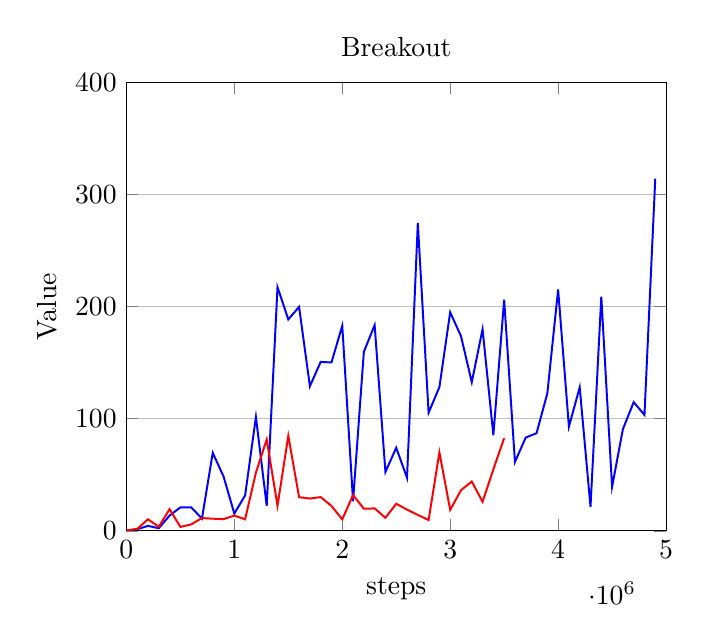
\begin{tikzpicture}

\begin{axis}[%
legend entries={rl-only-small-net,L2-reg,parallel-fs-50-no-aug}, 
legend columns=2,
title=Breakout,
legend to name=named,
legend style={legend cell align=left},
%%width=10in,
%%height=5in,
%%at={(2.596in,2.358in)},
% scale only axis,
xmin=0,
xmax=5000000,
xlabel style={font=\color{white!15!black}},
xlabel={steps},
xlabel near ticks,
ymin=0,
ymax=400,
ylabel style={font=\color{white!15!black}},
ylabel={Value},
ylabel near ticks,
ymajorgrids,
% %scale=0.5,
%%scale=0.4,
axis background/.style={fill=white},
%legend columns=2,
%legend=south outside
]
\addplot [color=blue, line width = 0.25mm]
                table[row sep=crcr]{
                  0 0.20000000298023224\\ 
100000 1.399999976158142\\ 
200000 4.400000095367432\\ 
300000 2.299999952316284\\ 
400000 13.600000381469727\\ 
500000 20.899999618530273\\ 
600000 21.0\\ 
700000 10.899999618530273\\ 
800000 69.5999984741211\\ 
900000 48.5\\ 
1000000 15.399999618530273\\ 
1100000 31.600000381469727\\ 
1200000 101.5999984741211\\ 
1300000 22.399999618530273\\ 
1400000 217.39999389648438\\ 
1500000 188.60000610351562\\ 
1600000 199.8000030517578\\ 
1700000 129.0\\ 
1800000 150.6999969482422\\ 
1900000 150.1999969482422\\ 
2000000 183.0\\ 
2100000 26.399999618530273\\ 
2200000 159.6999969482422\\ 
2300000 183.5\\ 
2400000 52.5\\ 
2500000 74.0999984741211\\ 
2600000 47.29999923706055\\ 
2700000 274.6000061035156\\ 
2800000 105.4000015258789\\ 
2900000 128.1999969482422\\ 
3000000 195.0\\ 
3100000 173.6999969482422\\ 
3200000 132.60000610351562\\ 
3300000 179.89999389648438\\ 
3400000 85.19999694824219\\ 
3500000 206.1999969482422\\ 
3600000 61.5\\ 
3700000 83.19999694824219\\ 
3800000 87.0999984741211\\ 
3900000 122.5999984741211\\ 
4000000 215.3000030517578\\ 
4100000 92.9000015258789\\ 
4200000 128.0\\ 
4300000 21.399999618530273\\ 
4400000 208.89999389648438\\ 
4500000 39.20000076293945\\ 
4600000 90.5999984741211\\ 
4700000 114.80000305175781\\ 
4800000 103.4000015258789\\ 
4900000 314.20001220703125\\ 
};
\addplot [color=red, line width = 0.25mm]
                table[row sep=crcr]{
                  0 0.4000000059604645\\ 
100000 1.7000000476837158\\ 
200000 10.300000190734863\\ 
300000 3.5999999046325684\\ 
400000 19.299999237060547\\ 
500000 3.5\\ 
600000 5.699999809265137\\ 
700000 11.399999618530273\\ 
800000 10.800000190734863\\ 
900000 10.399999618530273\\ 
1000000 13.600000381469727\\ 
1100000 10.300000190734863\\ 
1200000 51.900001525878906\\ 
1300000 81.5\\ 
1400000 22.299999237060547\\ 
1500000 84.69999694824219\\ 
1600000 30.0\\ 
1700000 28.799999237060547\\ 
1800000 30.100000381469727\\ 
1900000 22.200000762939453\\ 
2000000 10.199999809265137\\ 
2100000 31.899999618530273\\ 
2200000 19.700000762939453\\ 
2300000 20.0\\ 
2400000 11.600000381469727\\ 
2500000 24.200000762939453\\ 
2600000 18.899999618530273\\ 
2700000 14.199999809265137\\ 
2800000 9.600000381469727\\ 
2900000 70.0\\ 
3000000 18.700000762939453\\ 
3100000 36.20000076293945\\ 
3200000 44.0\\ 
3300000 25.899999618530273\\ 
3400000 54.900001525878906\\ 
3500000 82.69999694824219\\ 
};
\addplot [color=yellow, line width = 0.25mm]
                table[row sep=crcr]{
                  0 0.800000011920929\\ 
};
\end{axis}
\end{tikzpicture}}}
    \subfloat[]{  \resizebox{0.4\textwidth}{!}{
%\definecolor{blue}{RGB}{76,100,135}
%\definecolor{red}{RGB}{153,0,0}
%\definecolor{yellow}{RGB}{227,178,60}
%\definecolor{mycolor1}{rgb}{0.00000,0.44700,0.74100}%
%\definecolor{mycolor2}{rgb}{0.85000,0.32500,0.09800}%
%\definecolor{mycolor3}{rgb}{0.92900,0.69400,0.12500}%
%
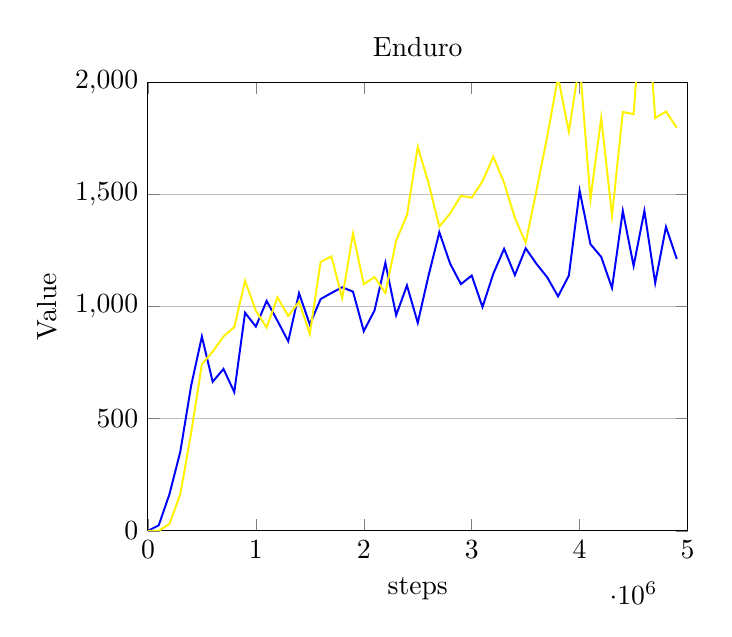
\begin{tikzpicture}

\begin{axis}[%
title=Enduro,
% %width=4.634in,
%%width=10in,
%%height=5in,
%at={(2.596in,2.358in)},
% scale only axis,
xmin=0,
xmax=5000000,
xlabel style={font=\color{white!15!black}},
xlabel={steps},
xlabel near ticks,
ymin=0,
ymax=2000,
ylabel style={font=\color{white!15!black}},
ylabel={Value},
ylabel near ticks,
ymajorgrids,
% %scale=0.5,
%scale=0.4,
axis background/.style={fill=white},
%legend style={legend cell align=left, align=left, draw=white!15!black}
]
\addplot [color=blue, line width = 0.25mm]
                table[row sep=crcr]{
                  0 0.0\\ 
100000 24.299999237060547\\ 
200000 164.3000030517578\\ 
300000 353.0\\ 
400000 646.4000244140625\\ 
500000 866.7000122070312\\ 
600000 664.7000122070312\\ 
700000 722.2000122070312\\ 
800000 618.9000244140625\\ 
900000 972.7999877929688\\ 
1000000 910.9000244140625\\ 
1100000 1025.699951171875\\ 
1200000 937.0\\ 
1300000 845.5999755859375\\ 
1400000 1059.9000244140625\\ 
1500000 920.2999877929688\\ 
1600000 1033.800048828125\\ 
1700000 1061.0\\ 
1800000 1086.5999755859375\\ 
1900000 1066.9000244140625\\ 
2000000 890.9000244140625\\ 
2100000 983.5\\ 
2200000 1195.300048828125\\ 
2300000 962.0\\ 
2400000 1094.800048828125\\ 
2500000 928.0\\ 
2600000 1138.5999755859375\\ 
2700000 1332.300048828125\\ 
2800000 1191.800048828125\\ 
2900000 1100.5999755859375\\ 
3000000 1138.800048828125\\ 
3100000 998.2999877929688\\ 
3200000 1146.800048828125\\ 
3300000 1258.0999755859375\\ 
3400000 1141.0\\ 
3500000 1260.300048828125\\ 
3600000 1190.800048828125\\ 
3700000 1130.5999755859375\\ 
3800000 1046.0999755859375\\ 
3900000 1138.4000244140625\\ 
4000000 1517.5\\ 
4100000 1278.9000244140625\\ 
4200000 1221.699951171875\\ 
4300000 1083.199951171875\\ 
4400000 1426.9000244140625\\ 
4500000 1181.5999755859375\\ 
4600000 1427.199951171875\\ 
4700000 1105.800048828125\\ 
4800000 1355.800048828125\\ 
4900000 1212.9000244140625\\ 
};
\addplot [color=red, line width = 0.25mm]
                table[row sep=crcr]{
                  0 0.0\\ 
};
\addplot [color=yellow, line width = 0.25mm]
                table[row sep=crcr]{
                  0 0.0\\ 
100000 0.0\\ 
200000 30.700000762939453\\ 
300000 163.6999969482422\\ 
400000 435.79998779296875\\ 
500000 743.2000122070312\\ 
600000 799.2000122070312\\ 
700000 867.0\\ 
800000 908.4000244140625\\ 
900000 1115.300048828125\\ 
1000000 981.4000244140625\\ 
1100000 906.9000244140625\\ 
1200000 1041.5999755859375\\ 
1300000 958.5999755859375\\ 
1400000 1021.9000244140625\\ 
1500000 877.7000122070312\\ 
1600000 1199.4000244140625\\ 
1700000 1224.0\\ 
1800000 1038.199951171875\\ 
1900000 1326.0999755859375\\ 
2000000 1100.0\\ 
2100000 1132.0999755859375\\ 
2200000 1060.9000244140625\\ 
2300000 1294.300048828125\\ 
2400000 1407.699951171875\\ 
2500000 1712.5\\ 
2600000 1551.5\\ 
2700000 1357.0\\ 
2800000 1415.800048828125\\ 
2900000 1494.5\\ 
3000000 1486.0\\ 
3100000 1559.699951171875\\ 
3200000 1668.5\\ 
3300000 1552.800048828125\\ 
3400000 1395.800048828125\\ 
3500000 1284.9000244140625\\ 
3600000 1518.0\\ 
3700000 1759.5999755859375\\ 
3800000 2024.9000244140625\\ 
3900000 1780.0999755859375\\ 
4000000 2090.5\\ 
4100000 1479.0999755859375\\ 
4200000 1841.699951171875\\ 
4300000 1405.5999755859375\\ 
4400000 1868.300048828125\\ 
4500000 1858.699951171875\\ 
4600000 2527.0\\ 
4700000 1841.0\\ 
4800000 1870.800048828125\\ 
4900000 1797.9000244140625\\ 
};
\end{axis}
\end{tikzpicture}}}\\
  \vspace{-1cm}
    \subfloat[]{  \resizebox{0.4\textwidth}{!}{
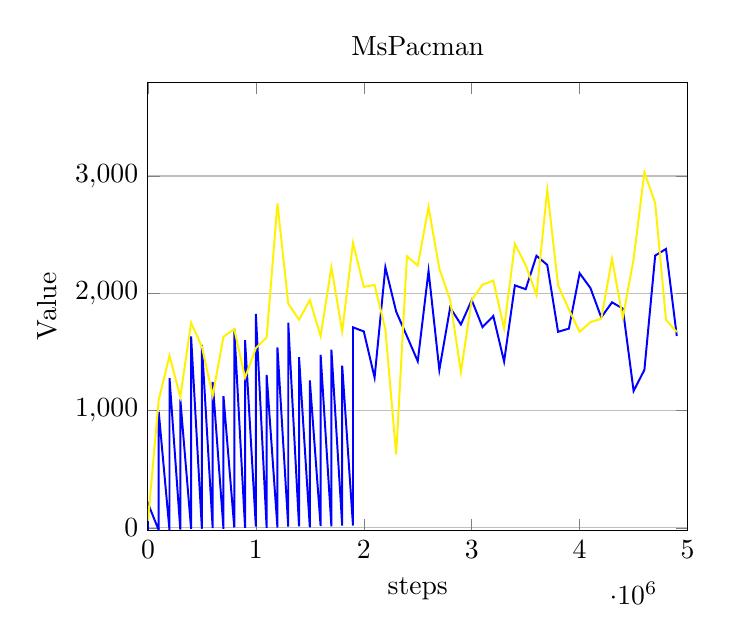
\begin{tikzpicture}

\begin{axis}[%
title=MsPacman,
% %width=4.634in,
%width=10in,
%height=5in,
%at={(2.596in,2.358in)},
% scale only axis,
xmin=0,
xmax=5000000,
xlabel style={font=\color{white!15!black}},
xlabel={steps},
xlabel near ticks,
ymin=-22,
ymax=3800,
ylabel style={font=\color{white!15!black}},
ylabel={Value},
ylabel near ticks,
ymajorgrids,
% %scale=0.5,
%scale=0.4,
axis background/.style={fill=white},
%legend style={legend cell align=left, align=left, draw=white!15!black}
]
\addplot [color=blue, line width = 0.25mm]
                table[row sep=crcr]{
                  0 -21.0\\ 
0 210.0\\ 
100000 -19.799999237060547\\ 
100000 990.0\\ 
200000 -20.700000762939453\\ 
200000 1277.0\\ 
300000 -15.0\\ 
300000 1096.0\\ 
400000 -7.0\\ 
400000 1632.0\\ 
500000 -6.900000095367432\\ 
500000 1561.0\\ 
600000 -1.899999976158142\\ 
600000 1245.0\\ 
700000 -7.599999904632568\\ 
700000 1123.0\\ 
800000 4.0\\ 
800000 1696.0\\ 
900000 1.5\\ 
900000 1600.0\\ 
1000000 11.300000190734863\\ 
1000000 1824.0\\ 
1100000 1.2000000476837158\\ 
1100000 1304.0\\ 
1200000 3.700000047683716\\ 
1200000 1538.0\\ 
1300000 11.5\\ 
1300000 1750.0\\ 
1400000 13.600000381469727\\ 
1400000 1456.0\\ 
1500000 5.699999809265137\\ 
1500000 1258.0\\ 
1600000 15.600000381469727\\ 
1600000 1476.0\\ 
1700000 13.5\\ 
1700000 1519.0\\ 
1800000 19.299999237060547\\ 
1800000 1383.0\\ 
1900000 20.799999237060547\\ 
1900000 1710.0\\ 
2000000 1675.0\\ 
2100000 1282.0\\ 
2200000 2222.0\\ 
2300000 1844.0\\ 
2400000 1634.0\\ 
2500000 1421.0\\ 
2600000 2191.0\\ 
2700000 1347.0\\ 
2800000 1878.0\\ 
2900000 1735.0\\ 
3000000 1942.0\\ 
3100000 1712.0\\ 
3200000 1806.0\\ 
3300000 1419.0\\ 
3400000 2068.0\\ 
3500000 2035.0\\ 
3600000 2320.0\\ 
3700000 2242.0\\ 
3800000 1672.0\\ 
3900000 1699.0\\ 
4000000 2171.0\\ 
4100000 2045.0\\ 
4200000 1795.0\\ 
4300000 1923.0\\ 
4400000 1870.0\\ 
4500000 1167.0\\ 
4600000 1348.0\\ 
4700000 2322.0\\ 
4800000 2378.0\\ 
4900000 1636.0\\ 
};
\addplot [color=red, line width = 0.25mm]
                table[row sep=crcr]{
                  0 0.0\\ 
};
\addplot [color=yellow, line width = 0.25mm]
                table[row sep=crcr]{
                  0 60.0\\ 
100000 1090.0\\ 
200000 1469.0\\ 
300000 1117.0\\ 
400000 1749.0\\ 
500000 1545.0\\ 
600000 1128.0\\ 
700000 1630.0\\ 
800000 1695.0\\ 
900000 1281.0\\ 
1000000 1532.0\\ 
1100000 1625.0\\ 
1200000 2767.0\\ 
1300000 1912.0\\ 
1400000 1775.0\\ 
1500000 1942.0\\ 
1600000 1636.0\\ 
1700000 2222.0\\ 
1800000 1676.0\\ 
1900000 2430.0\\ 
2000000 2055.0\\ 
2100000 2072.0\\ 
2200000 1693.0\\ 
2300000 625.0\\ 
2400000 2317.0\\ 
2500000 2236.0\\ 
2600000 2736.0\\ 
2700000 2209.0\\ 
2800000 1944.0\\ 
2900000 1329.0\\ 
3000000 1944.0\\ 
3100000 2074.0\\ 
3200000 2109.0\\ 
3300000 1701.0\\ 
3400000 2421.0\\ 
3500000 2240.0\\ 
3600000 1986.0\\ 
3700000 2883.0\\ 
3800000 2069.0\\ 
3900000 1863.0\\ 
4000000 1672.0\\ 
4100000 1754.0\\ 
4200000 1783.0\\ 
4300000 2293.0\\ 
4400000 1791.0\\ 
4500000 2293.0\\ 
4600000 3033.0\\ 
4700000 2768.0\\ 
4800000 1774.0\\ 
4900000 1670.0\\ 
};
\end{axis}
\end{tikzpicture}}}
    \subfloat[]{  \resizebox{0.4\textwidth}{!}{
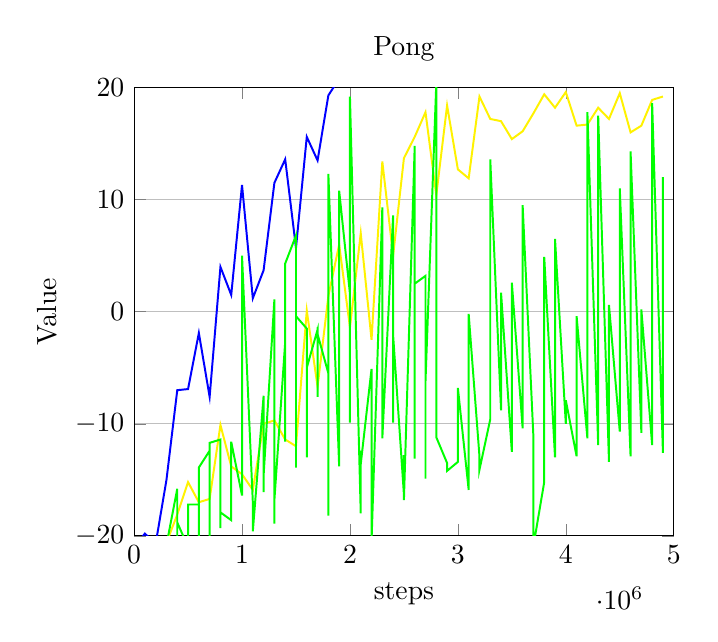
\begin{tikzpicture}

\begin{axis}[%
title=Pong,
% %width=4.634in,
%width=10in,
%height=5in,
%at={(2.596in,2.358in)},
% scale only axis,
xmin=0,
xmax=5000000,
xlabel style={font=\color{white!15!black}},
xlabel={steps},
xlabel near ticks,
ymin=-20,
ymax=20,
ylabel style={font=\color{white!15!black}},
ylabel={Value},
ylabel near ticks,
ymajorgrids,
% %scale=0.5,
%scale=0.4,
axis background/.style={fill=white},
%legend style={legend cell align=left, align=left, draw=white!15!black}
]
\addplot [color=blue, line width = 0.25mm]
                table[row sep=crcr]{
                  0 -21.0\\ 
100000 -19.799999237060547\\ 
200000 -20.700000762939453\\ 
300000 -15.0\\ 
400000 -7.0\\ 
500000 -6.900000095367432\\ 
600000 -1.899999976158142\\ 
700000 -7.599999904632568\\ 
800000 4.0\\ 
900000 1.5\\ 
1000000 11.300000190734863\\ 
1100000 1.2000000476837158\\ 
1200000 3.700000047683716\\ 
1300000 11.5\\ 
1400000 13.600000381469727\\ 
1500000 5.699999809265137\\ 
1600000 15.600000381469727\\ 
1700000 13.5\\ 
1800000 19.299999237060547\\ 
1900000 20.799999237060547\\ 
};
\addplot [color=red, line width = 0.25mm]
                table[row sep=crcr]{
                  0 0.0\\ 
};
\addplot [color=yellow, line width = 0.25mm]
                table[row sep=crcr]{
                  0 -21.0\\ 
0 -21.0\\ 
0 -21.0\\ 
100000 -21.0\\ 
200000 -20.299999237060547\\ 
300000 -20.600000381469727\\ 
400000 -18.100000381469727\\ 
500000 -15.199999809265137\\ 
600000 -17.0\\ 
700000 -16.700000762939453\\ 
800000 -10.100000381469727\\ 
900000 -13.800000190734863\\ 
1000000 -14.5\\ 
1100000 -15.899999618530273\\ 
1200000 -10.0\\ 
1300000 -9.699999809265137\\ 
1400000 -11.399999618530273\\ 
1500000 -12.0\\ 
1600000 0.10000000149011612\\ 
1700000 -6.699999809265137\\ 
1800000 1.399999976158142\\ 
1900000 6.0\\ 
2000000 -1.399999976158142\\ 
2100000 7.0\\ 
2200000 -2.5\\ 
2300000 13.399999618530273\\ 
2400000 5.0\\ 
2500000 13.699999809265137\\ 
2600000 15.600000381469727\\ 
2700000 17.799999237060547\\ 
2800000 10.399999618530273\\ 
2900000 18.399999618530273\\ 
3000000 12.699999809265137\\ 
3100000 11.899999618530273\\ 
3200000 19.200000762939453\\ 
3300000 17.200000762939453\\ 
3400000 17.0\\ 
3500000 15.399999618530273\\ 
3600000 16.100000381469727\\ 
3700000 17.700000762939453\\ 
3800000 19.399999618530273\\ 
3900000 18.200000762939453\\ 
4000000 19.600000381469727\\ 
4100000 16.600000381469727\\ 
4200000 16.700000762939453\\ 
4300000 18.200000762939453\\ 
4400000 17.200000762939453\\ 
4500000 19.5\\ 
4600000 16.0\\ 
4700000 16.600000381469727\\ 
4800000 18.899999618530273\\ 
4900000 19.200000762939453\\ 
};
\addplot [color=green, line width = 0.25mm]
                table[row sep=crcr]{
                  0 -21.0\\ 
0 -21.0\\ 
0 -21.0\\ 
0 -21.0\\ 
100000 -21.0\\ 
100000 -20.600000381469727\\ 
100000 -21.0\\ 
200000 -20.399999618530273\\ 
200000 -21.0\\ 
200000 -20.799999237060547\\ 
300000 -20.600000381469727\\ 
300000 -20.799999237060547\\ 
300000 -20.799999237060547\\ 
400000 -15.800000190734863\\ 
400000 -20.399999618530273\\ 
400000 -18.799999237060547\\ 
500000 -21.0\\ 
500000 -21.0\\ 
500000 -17.200000762939453\\ 
600000 -17.200000762939453\\ 
600000 -20.600000381469727\\ 
600000 -13.899999618530273\\ 
700000 -12.399999618530273\\ 
700000 -20.100000381469727\\ 
700000 -11.699999809265137\\ 
800000 -11.399999618530273\\ 
800000 -19.299999237060547\\ 
800000 -17.899999618530273\\ 
900000 -18.600000381469727\\ 
900000 -15.699999809265137\\ 
900000 -11.600000381469727\\ 
1000000 -16.399999618530273\\ 
1000000 -16.0\\ 
1000000 5.0\\ 
1100000 -17.0\\ 
1100000 -17.5\\ 
1100000 -19.600000381469727\\ 
1200000 -7.5\\ 
1200000 -16.100000381469727\\ 
1200000 -14.600000381469727\\ 
1300000 1.100000023841858\\ 
1300000 -18.899999618530273\\ 
1300000 -16.799999237060547\\ 
1400000 -2.700000047683716\\ 
1400000 -11.600000381469727\\ 
1400000 4.300000190734863\\ 
1500000 6.800000190734863\\ 
1500000 -13.899999618530273\\ 
1500000 -0.4000000059604645\\ 
1600000 -1.5\\ 
1600000 -13.0\\ 
1600000 -5.0\\ 
1700000 -1.600000023841858\\ 
1700000 -7.599999904632568\\ 
1700000 -2.0\\ 
1800000 -5.5\\ 
1800000 -18.200000762939453\\ 
1800000 12.300000190734863\\ 
1900000 -13.800000190734863\\ 
1900000 -10.0\\ 
1900000 10.800000190734863\\ 
2000000 1.600000023841858\\ 
2000000 -9.899999618530273\\ 
2000000 19.200000762939453\\ 
2100000 -18.0\\ 
2100000 -12.399999618530273\\ 
2100000 -13.600000381469727\\ 
2200000 -5.099999904632568\\ 
2200000 -13.899999618530273\\ 
2200000 -20.5\\ 
2300000 9.300000190734863\\ 
2300000 -8.199999809265137\\ 
2300000 -11.300000190734863\\ 
2400000 8.600000381469727\\ 
2400000 -9.899999618530273\\ 
2400000 -2.0999999046325684\\ 
2500000 -16.299999237060547\\ 
2500000 -12.800000190734863\\ 
2500000 -16.799999237060547\\ 
2600000 14.800000190734863\\ 
2600000 -13.100000381469727\\ 
2600000 2.5\\ 
2700000 3.200000047683716\\ 
2700000 -14.899999618530273\\ 
2700000 -6.199999809265137\\ 
2800000 20.399999618530273\\ 
2800000 -9.800000190734863\\ 
2800000 -11.199999809265137\\ 
2900000 -13.5\\ 
2900000 -14.199999809265137\\ 
3000000 -13.399999618530273\\ 
3000000 -6.800000190734863\\ 
3100000 -15.899999618530273\\ 
3100000 -0.20000000298023224\\ 
3200000 -12.899999618530273\\ 
3200000 -14.100000381469727\\ 
3300000 -9.600000381469727\\ 
3300000 13.600000381469727\\ 
3400000 -8.800000190734863\\ 
3400000 1.7000000476837158\\ 
3500000 -12.5\\ 
3500000 2.5999999046325684\\ 
3600000 -10.399999618530273\\ 
3600000 9.5\\ 
3700000 -11.199999809265137\\ 
3700000 -20.899999618530273\\ 
3800000 -15.199999809265137\\ 
3800000 4.900000095367432\\ 
3900000 -13.0\\ 
3900000 6.5\\ 
4000000 -10.0\\ 
4000000 -7.900000095367432\\ 
4100000 -12.899999618530273\\ 
4100000 -0.4000000059604645\\ 
4200000 -11.300000190734863\\ 
4200000 17.799999237060547\\ 
4300000 -11.899999618530273\\ 
4300000 17.5\\ 
4400000 -13.399999618530273\\ 
4400000 0.6000000238418579\\ 
4500000 -10.699999809265137\\ 
4500000 11.0\\ 
4600000 -12.899999618530273\\ 
4600000 14.300000190734863\\ 
4700000 -10.800000190734863\\ 
4700000 0.20000000298023224\\ 
4800000 -11.899999618530273\\ 
4800000 18.600000381469727\\ 
4900000 -12.600000381469727\\ 
4900000 12.0\\ 
};
\end{axis}
\end{tikzpicture}}}\\
    \ref{named}
%  \label{fig:rl-only-vs-pretrained}
\end{figure}
\end{frame}


\begin{frame}[plain]
		\centering
		\underline{Effectiveness of parallel training --- continued}
		\vspace{-1cm}
\begin{figure}[!t]
  \captionsetup[subfloat]{position=top,labelformat=empty}
  \centering
    \subfloat[]{  \resizebox{0.4\textwidth}{!}{
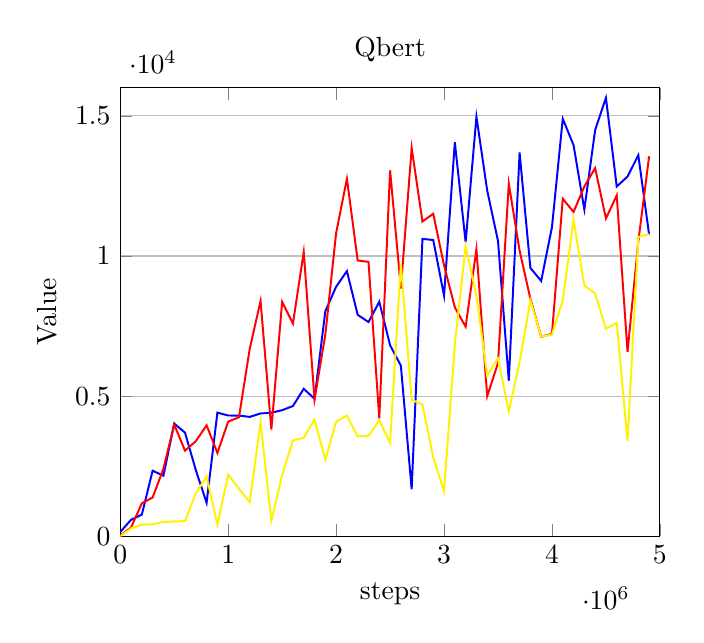
\begin{tikzpicture}

\begin{axis}[%
title=Qbert,
% %width=4.634in,
%width=10in,
%height=5in,
%at={(2.596in,2.358in)},
% scale only axis,
xmin=0,
xmax=5000000,
xlabel style={font=\color{white!15!black}},
xlabel={steps},
xlabel near ticks,
ymin=0,
ymax=16000,
ylabel style={font=\color{white!15!black}},
ylabel={Value},
ylabel near ticks,
ymajorgrids,
% %scale=0.5,
%scale=0.4,
axis background/.style={fill=white},
%legend style={legend cell align=left, align=left, draw=white!15!black}
]
\addplot [color=blue, line width = 0.25mm]
                table[row sep=crcr]{
                  0 150.0\\ 
100000 585.0\\ 
200000 772.5\\ 
300000 2337.5\\ 
400000 2157.5\\ 
500000 4022.5\\ 
600000 3695.0\\ 
700000 2362.5\\ 
800000 1192.5\\ 
900000 4410.0\\ 
1000000 4307.5\\ 
1100000 4305.0\\ 
1200000 4257.5\\ 
1300000 4380.0\\ 
1400000 4407.5\\ 
1500000 4497.5\\ 
1600000 4645.0\\ 
1700000 5260.0\\ 
1800000 4905.0\\ 
1900000 8030.0\\ 
2000000 8902.5\\ 
2100000 9460.0\\ 
2200000 7900.0\\ 
2300000 7642.5\\ 
2400000 8367.5\\ 
2500000 6815.0\\ 
2600000 6085.0\\ 
2700000 1677.5\\ 
2800000 10610.0\\ 
2900000 10570.0\\ 
3000000 8585.0\\ 
3100000 14057.5\\ 
3200000 10490.0\\ 
3300000 14970.0\\ 
3400000 12332.5\\ 
3500000 10537.5\\ 
3600000 5550.0\\ 
3700000 13692.5\\ 
3800000 9572.5\\ 
3900000 9110.0\\ 
4000000 11030.0\\ 
4100000 14897.5\\ 
4200000 13955.0\\ 
4300000 11660.0\\ 
4400000 14495.0\\ 
4500000 15645.0\\ 
4600000 12480.0\\ 
4700000 12835.0\\ 
4800000 13597.5\\ 
4900000 10762.5\\ 
};
\addplot [color=red, line width = 0.25mm]
                table[row sep=crcr]{
                  0 22.5\\ 
100000 310.0\\ 
200000 1172.5\\ 
300000 1382.5\\ 
400000 2410.0\\ 
500000 3982.5\\ 
600000 3052.5\\ 
700000 3390.0\\ 
800000 3957.5\\ 
900000 2970.0\\ 
1000000 4090.0\\ 
1100000 4245.0\\ 
1200000 6697.5\\ 
1300000 8395.0\\ 
1400000 3807.5\\ 
1500000 8360.0\\ 
1600000 7590.0\\ 
1700000 10142.5\\ 
1800000 4877.5\\ 
1900000 7190.0\\ 
2000000 10817.5\\ 
2100000 12755.0\\ 
2200000 9840.0\\ 
2300000 9790.0\\ 
2400000 4202.5\\ 
2500000 13057.5\\ 
2600000 8842.5\\ 
2700000 13852.5\\ 
2800000 11230.0\\ 
2900000 11507.5\\ 
3000000 9665.0\\ 
3100000 8167.5\\ 
3200000 7475.0\\ 
3300000 10242.5\\ 
3400000 4997.5\\ 
3500000 6180.0\\ 
3600000 12582.5\\ 
3700000 10190.0\\ 
3800000 8475.0\\ 
3900000 7115.0\\ 
4000000 7222.5\\ 
4100000 12042.5\\ 
4200000 11572.5\\ 
4300000 12480.0\\ 
4400000 13137.5\\ 
4500000 11337.5\\ 
4600000 12165.0\\ 
4700000 6580.0\\ 
4800000 10517.5\\ 
4900000 13560.0\\ 
};
\addplot [color=yellow, line width = 0.25mm]
                table[row sep=crcr]{
                  0 0.0\\ 
100000 280.0\\ 
200000 415.0\\ 
300000 425.0\\ 
400000 507.5\\ 
500000 525.0\\ 
600000 537.5\\ 
700000 1525.0\\ 
800000 2137.5\\ 
900000 407.5\\ 
1000000 2195.0\\ 
1100000 1690.0\\ 
1200000 1215.0\\ 
1300000 4077.5\\ 
1400000 550.0\\ 
1500000 2185.0\\ 
1600000 3417.5\\ 
1700000 3512.5\\ 
1800000 4165.0\\ 
1900000 2730.0\\ 
2000000 4090.0\\ 
2100000 4305.0\\ 
2200000 3557.5\\ 
2300000 3585.0\\ 
2400000 4137.5\\ 
2500000 3335.0\\ 
2600000 9722.5\\ 
2700000 4865.0\\ 
2800000 4700.0\\ 
2900000 2812.5\\ 
3000000 1605.0\\ 
3100000 6847.5\\ 
3200000 10342.5\\ 
3300000 8590.0\\ 
3400000 5732.5\\ 
3500000 6345.0\\ 
3600000 4447.5\\ 
3700000 6217.5\\ 
3800000 8415.0\\ 
3900000 7120.0\\ 
4000000 7195.0\\ 
4100000 8415.0\\ 
4200000 11307.5\\ 
4300000 8942.5\\ 
4400000 8662.5\\ 
4500000 7402.5\\ 
4600000 7612.5\\ 
4700000 3395.0\\ 
4800000 10680.0\\ 
4900000 10780.0\\ 
};
\end{axis}
\end{tikzpicture}}}
    \subfloat[]{  \resizebox{0.4\textwidth}{!}{
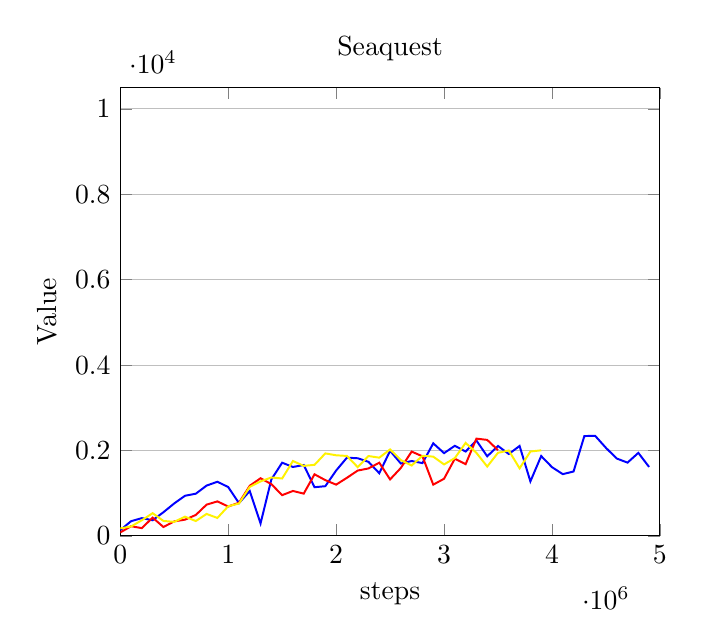
\begin{tikzpicture}

\begin{axis}[%
title=Seaquest,
% %width=4.634in,
%width=10in,
%height=5in,
%at={(2.596in,2.358in)},
% scale only axis,
xmin=0,
xmax=5000000,
xlabel style={font=\color{white!15!black}},
xlabel={steps},
xlabel near ticks,
ymin=0,
ymax=10500,
ylabel style={font=\color{white!15!black}},
ylabel={Value},
ylabel near ticks,
ymajorgrids,
% %scale=0.5,
%scale=0.4,
axis background/.style={fill=white},
%legend style={legend cell align=left, align=left, draw=white!15!black}
]
\addplot [color=blue, line width = 0.25mm]
                table[row sep=crcr]{
                  0 134.0\\ 
100000 344.0\\ 
200000 416.0\\ 
300000 366.0\\ 
400000 554.0\\ 
500000 760.0\\ 
600000 940.0\\ 
700000 988.0\\ 
800000 1178.0\\ 
900000 1268.0\\ 
1000000 1144.0\\ 
1100000 768.0\\ 
1200000 1052.0\\ 
1300000 292.0\\ 
1400000 1322.0\\ 
1500000 1714.0\\ 
1600000 1614.0\\ 
1700000 1660.0\\ 
1800000 1140.0\\ 
1900000 1164.0\\ 
2000000 1530.0\\ 
2100000 1832.0\\ 
2200000 1818.0\\ 
2300000 1734.0\\ 
2400000 1468.0\\ 
2500000 1992.0\\ 
2600000 1694.0\\ 
2700000 1754.0\\ 
2800000 1704.0\\ 
2900000 2168.0\\ 
3000000 1938.0\\ 
3100000 2110.0\\ 
3200000 1976.0\\ 
3300000 2234.0\\ 
3400000 1864.0\\ 
3500000 2106.0\\ 
3600000 1918.0\\ 
3700000 2106.0\\ 
3800000 1276.0\\ 
3900000 1870.0\\ 
4000000 1610.0\\ 
4100000 1446.0\\ 
4200000 1508.0\\ 
4300000 2338.0\\ 
4400000 2344.0\\ 
4500000 2062.0\\ 
4600000 1812.0\\ 
4700000 1716.0\\ 
4800000 1944.0\\ 
4900000 1614.0\\ 
};
\addplot [color=red, line width = 0.25mm]
                table[row sep=crcr]{
                  0 80.0\\ 
100000 226.0\\ 
200000 182.0\\ 
300000 428.0\\ 
400000 208.0\\ 
500000 340.0\\ 
600000 380.0\\ 
700000 490.0\\ 
800000 732.0\\ 
900000 808.0\\ 
1000000 688.0\\ 
1100000 776.0\\ 
1200000 1174.0\\ 
1300000 1350.0\\ 
1400000 1212.0\\ 
1500000 954.0\\ 
1600000 1052.0\\ 
1700000 990.0\\ 
1800000 1442.0\\ 
1900000 1306.0\\ 
2000000 1200.0\\ 
2100000 1360.0\\ 
2200000 1530.0\\ 
2300000 1580.0\\ 
2400000 1714.0\\ 
2500000 1322.0\\ 
2600000 1592.0\\ 
2700000 1974.0\\ 
2800000 1864.0\\ 
2900000 1200.0\\ 
3000000 1338.0\\ 
3100000 1808.0\\ 
3200000 1680.0\\ 
3300000 2278.0\\ 
3400000 2248.0\\ 
3500000 2008.0\\ 
};
\addplot [color=yellow, line width = 0.25mm]
                table[row sep=crcr]{
                  0 176.0\\ 
100000 220.0\\ 
200000 366.0\\ 
300000 532.0\\ 
400000 350.0\\ 
500000 328.0\\ 
600000 450.0\\ 
700000 348.0\\ 
800000 514.0\\ 
900000 420.0\\ 
1000000 694.0\\ 
1100000 758.0\\ 
1200000 1148.0\\ 
1300000 1276.0\\ 
1400000 1368.0\\ 
1500000 1344.0\\ 
1600000 1754.0\\ 
1700000 1640.0\\ 
1800000 1664.0\\ 
1900000 1932.0\\ 
2000000 1888.0\\ 
2100000 1872.0\\ 
2200000 1610.0\\ 
2300000 1870.0\\ 
2400000 1832.0\\ 
2500000 2024.0\\ 
2600000 1774.0\\ 
2700000 1648.0\\ 
2800000 1876.0\\ 
2900000 1856.0\\ 
3000000 1674.0\\ 
3100000 1822.0\\ 
3200000 2178.0\\ 
3300000 1944.0\\ 
3400000 1624.0\\ 
3500000 1946.0\\ 
3600000 2000.0\\ 
3700000 1582.0\\ 
3800000 1976.0\\ 
3900000 2004.0\\ 
};
\end{axis}
\end{tikzpicture}}}\\
  \vspace{-1cm}
    \subfloat[]{  \resizebox{0.4\textwidth}{!}{
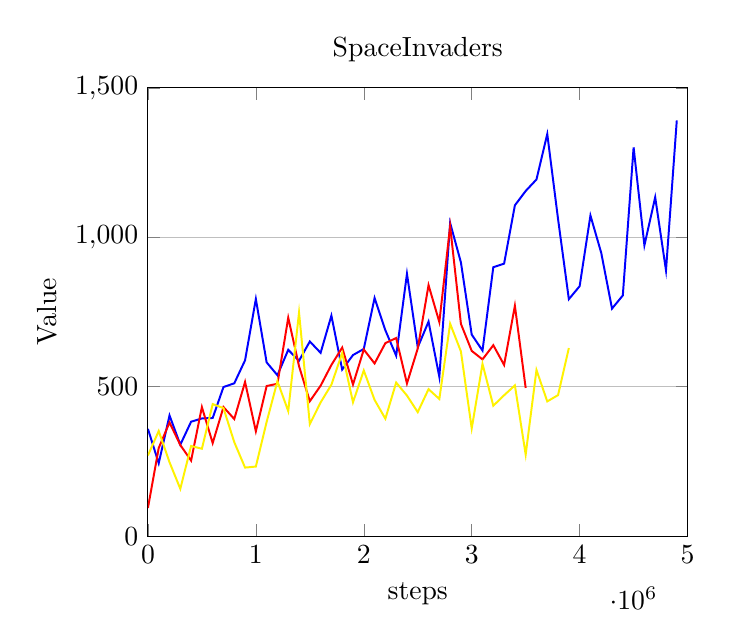
\begin{tikzpicture}

\begin{axis}[%
title=SpaceInvaders,
%width=10in,
%height=5in,
%at={(2.596in,2.358in)},
% scale only axis,
xmin=0,
xmax=5000000,
xlabel style={font=\color{white!15!black}},
xlabel={steps},
xlabel near ticks,
ymin=0,
ymax=1500,
ylabel style={font=\color{white!15!black}},
ylabel={Value},
ylabel near ticks,
ymajorgrids,
% %scale=0.5,
%scale=0.4,
axis background/.style={fill=white},
%legend style={legend cell align=left, align=left, draw=white!15!black}
]
\addplot [color=blue, line width = 0.25mm]
                table[row sep=crcr]{
                  0 359.0\\ 
100000 244.0\\ 
200000 404.0\\ 
300000 306.0\\ 
400000 383.0\\ 
500000 394.0\\ 
600000 395.5\\ 
700000 499.0\\ 
800000 511.5\\ 
900000 588.5\\ 
1000000 793.5\\ 
1100000 581.5\\ 
1200000 538.5\\ 
1300000 623.5\\ 
1400000 587.0\\ 
1500000 651.5\\ 
1600000 613.5\\ 
1700000 738.0\\ 
1800000 557.5\\ 
1900000 606.0\\ 
2000000 626.5\\ 
2100000 797.0\\ 
2200000 689.0\\ 
2300000 604.0\\ 
2400000 878.0\\ 
2500000 632.0\\ 
2600000 718.0\\ 
2700000 533.0\\ 
2800000 1048.0\\ 
2900000 916.0\\ 
3000000 674.5\\ 
3100000 621.0\\ 
3200000 900.0\\ 
3300000 912.0\\ 
3400000 1107.0\\ 
3500000 1155.0\\ 
3600000 1193.5\\ 
3700000 1345.5\\ 
3800000 1061.0\\ 
3900000 793.0\\ 
4000000 836.5\\ 
4100000 1073.0\\ 
4200000 948.0\\ 
4300000 761.5\\ 
4400000 805.5\\ 
4500000 1301.0\\ 
4600000 973.0\\ 
4700000 1134.0\\ 
4800000 889.5\\ 
4900000 1391.0\\ 
};
\addplot [color=red, line width = 0.25mm]
                table[row sep=crcr]{
                  0 94.5\\ 
100000 295.0\\ 
200000 380.5\\ 
300000 305.0\\ 
400000 253.0\\ 
500000 432.0\\ 
600000 311.5\\ 
700000 432.0\\ 
800000 392.0\\ 
900000 516.0\\ 
1000000 351.0\\ 
1100000 502.5\\ 
1200000 510.0\\ 
1300000 731.0\\ 
1400000 569.0\\ 
1500000 451.5\\ 
1600000 503.5\\ 
1700000 573.0\\ 
1800000 631.0\\ 
1900000 507.5\\ 
2000000 624.5\\ 
2100000 578.0\\ 
2200000 646.0\\ 
2300000 663.0\\ 
2400000 511.0\\ 
2500000 628.0\\ 
2600000 840.0\\ 
2700000 716.5\\ 
2800000 1037.0\\ 
2900000 710.5\\ 
3000000 620.0\\ 
3100000 591.5\\ 
3200000 639.0\\ 
3300000 573.0\\ 
3400000 771.0\\ 
3500000 496.0\\ 
};
\addplot [color=yellow, line width = 0.25mm]
                table[row sep=crcr]{
                  0 270.0\\ 
100000 352.0\\ 
200000 247.5\\ 
300000 158.5\\ 
400000 302.0\\ 
500000 292.5\\ 
600000 442.0\\ 
700000 428.5\\ 
800000 314.5\\ 
900000 229.5\\ 
1000000 233.0\\ 
1100000 382.5\\ 
1200000 518.5\\ 
1300000 418.5\\ 
1400000 748.5\\ 
1500000 375.0\\ 
1600000 447.5\\ 
1700000 507.0\\ 
1800000 613.0\\ 
1900000 448.0\\ 
2000000 554.5\\ 
2100000 456.0\\ 
2200000 393.0\\ 
2300000 514.0\\ 
2400000 470.5\\ 
2500000 415.0\\ 
2600000 492.0\\ 
2700000 459.0\\ 
2800000 711.0\\ 
2900000 618.0\\ 
3000000 360.5\\ 
3100000 576.5\\ 
3200000 436.5\\ 
3300000 471.5\\ 
3400000 504.5\\ 
3500000 273.0\\ 
3600000 556.0\\ 
3700000 451.0\\ 
3800000 472.0\\ 
3900000 629.5\\ 
};
\end{axis}
\end{tikzpicture}}}
  \\
    \ref{named}
\end{figure}
\end{frame}


\begin{frame}[plain]
		\centering
		\underline{Effectiveness of regularization}
		\vspace{-1cm}
\begin{figure}[!t]
  \captionsetup[subfloat]{position=top,labelformat=empty}
  \centering
    \subfloat[]{  \resizebox{0.4\textwidth}{!}{
%\definecolor{blue}{RGB}{76,100,135}
%\definecolor{red}{RGB}{153,0,0}
%\definecolor{yellow}{RGB}{227,178,60}
%\definecolor{mycolor1}{rgb}{0.00000,0.44700,0.74100}%
%\definecolor{mycolor2}{rgb}{0.85000,0.32500,0.09800}%
%\definecolor{mycolor3}{rgb}{0.92900,0.69400,0.12500}%
%
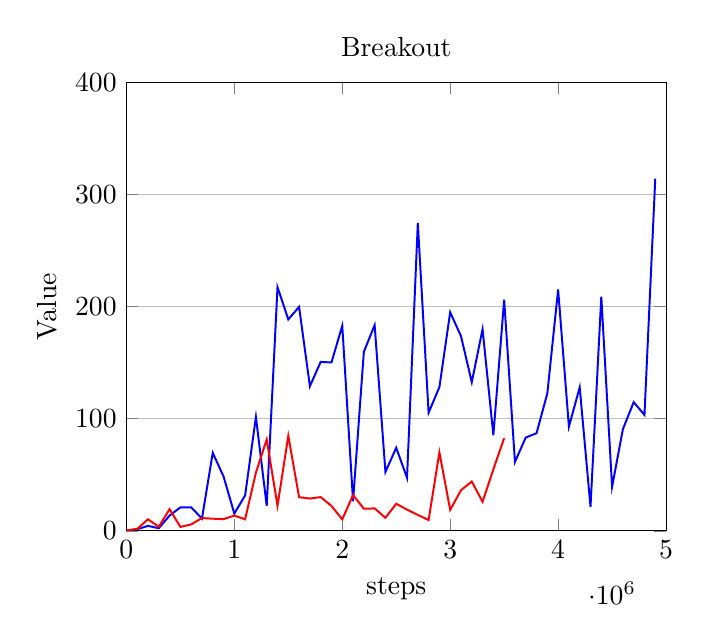
\begin{tikzpicture}

\begin{axis}[%
legend entries={rl-only-small-net,L2-reg,parallel-fs-50-no-aug}, 
legend columns=2,
title=Breakout,
legend to name=named,
legend style={legend cell align=left},
%%width=10in,
%%height=5in,
%%at={(2.596in,2.358in)},
% scale only axis,
xmin=0,
xmax=5000000,
xlabel style={font=\color{white!15!black}},
xlabel={steps},
xlabel near ticks,
ymin=0,
ymax=400,
ylabel style={font=\color{white!15!black}},
ylabel={Value},
ylabel near ticks,
ymajorgrids,
% %scale=0.5,
%%scale=0.4,
axis background/.style={fill=white},
%legend columns=2,
%legend=south outside
]
\addplot [color=blue, line width = 0.25mm]
                table[row sep=crcr]{
                  0 0.20000000298023224\\ 
100000 1.399999976158142\\ 
200000 4.400000095367432\\ 
300000 2.299999952316284\\ 
400000 13.600000381469727\\ 
500000 20.899999618530273\\ 
600000 21.0\\ 
700000 10.899999618530273\\ 
800000 69.5999984741211\\ 
900000 48.5\\ 
1000000 15.399999618530273\\ 
1100000 31.600000381469727\\ 
1200000 101.5999984741211\\ 
1300000 22.399999618530273\\ 
1400000 217.39999389648438\\ 
1500000 188.60000610351562\\ 
1600000 199.8000030517578\\ 
1700000 129.0\\ 
1800000 150.6999969482422\\ 
1900000 150.1999969482422\\ 
2000000 183.0\\ 
2100000 26.399999618530273\\ 
2200000 159.6999969482422\\ 
2300000 183.5\\ 
2400000 52.5\\ 
2500000 74.0999984741211\\ 
2600000 47.29999923706055\\ 
2700000 274.6000061035156\\ 
2800000 105.4000015258789\\ 
2900000 128.1999969482422\\ 
3000000 195.0\\ 
3100000 173.6999969482422\\ 
3200000 132.60000610351562\\ 
3300000 179.89999389648438\\ 
3400000 85.19999694824219\\ 
3500000 206.1999969482422\\ 
3600000 61.5\\ 
3700000 83.19999694824219\\ 
3800000 87.0999984741211\\ 
3900000 122.5999984741211\\ 
4000000 215.3000030517578\\ 
4100000 92.9000015258789\\ 
4200000 128.0\\ 
4300000 21.399999618530273\\ 
4400000 208.89999389648438\\ 
4500000 39.20000076293945\\ 
4600000 90.5999984741211\\ 
4700000 114.80000305175781\\ 
4800000 103.4000015258789\\ 
4900000 314.20001220703125\\ 
};
\addplot [color=red, line width = 0.25mm]
                table[row sep=crcr]{
                  0 0.4000000059604645\\ 
100000 1.7000000476837158\\ 
200000 10.300000190734863\\ 
300000 3.5999999046325684\\ 
400000 19.299999237060547\\ 
500000 3.5\\ 
600000 5.699999809265137\\ 
700000 11.399999618530273\\ 
800000 10.800000190734863\\ 
900000 10.399999618530273\\ 
1000000 13.600000381469727\\ 
1100000 10.300000190734863\\ 
1200000 51.900001525878906\\ 
1300000 81.5\\ 
1400000 22.299999237060547\\ 
1500000 84.69999694824219\\ 
1600000 30.0\\ 
1700000 28.799999237060547\\ 
1800000 30.100000381469727\\ 
1900000 22.200000762939453\\ 
2000000 10.199999809265137\\ 
2100000 31.899999618530273\\ 
2200000 19.700000762939453\\ 
2300000 20.0\\ 
2400000 11.600000381469727\\ 
2500000 24.200000762939453\\ 
2600000 18.899999618530273\\ 
2700000 14.199999809265137\\ 
2800000 9.600000381469727\\ 
2900000 70.0\\ 
3000000 18.700000762939453\\ 
3100000 36.20000076293945\\ 
3200000 44.0\\ 
3300000 25.899999618530273\\ 
3400000 54.900001525878906\\ 
3500000 82.69999694824219\\ 
};
\addplot [color=yellow, line width = 0.25mm]
                table[row sep=crcr]{
                  0 0.800000011920929\\ 
};
\end{axis}
\end{tikzpicture}}}
    \subfloat[]{  \resizebox{0.4\textwidth}{!}{
%\definecolor{blue}{RGB}{76,100,135}
%\definecolor{red}{RGB}{153,0,0}
%\definecolor{yellow}{RGB}{227,178,60}
%\definecolor{mycolor1}{rgb}{0.00000,0.44700,0.74100}%
%\definecolor{mycolor2}{rgb}{0.85000,0.32500,0.09800}%
%\definecolor{mycolor3}{rgb}{0.92900,0.69400,0.12500}%
%
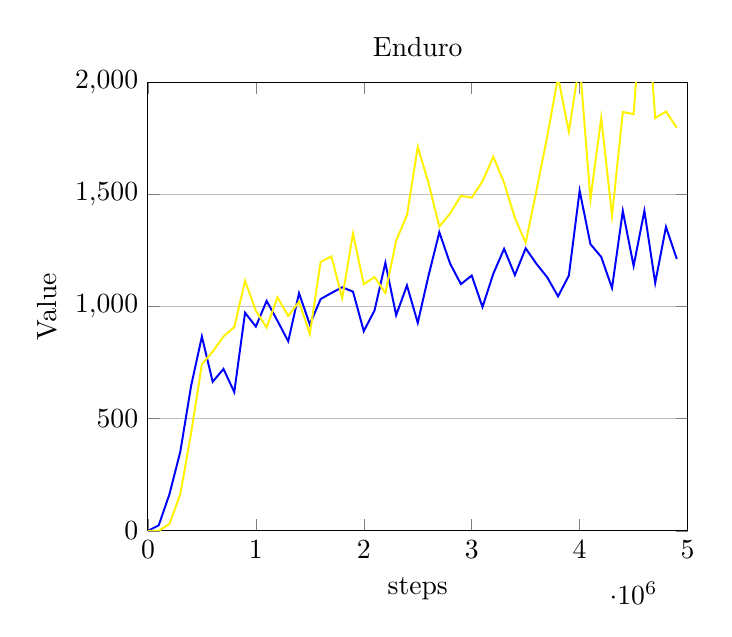
\begin{tikzpicture}

\begin{axis}[%
title=Enduro,
% %width=4.634in,
%%width=10in,
%%height=5in,
%at={(2.596in,2.358in)},
% scale only axis,
xmin=0,
xmax=5000000,
xlabel style={font=\color{white!15!black}},
xlabel={steps},
xlabel near ticks,
ymin=0,
ymax=2000,
ylabel style={font=\color{white!15!black}},
ylabel={Value},
ylabel near ticks,
ymajorgrids,
% %scale=0.5,
%scale=0.4,
axis background/.style={fill=white},
%legend style={legend cell align=left, align=left, draw=white!15!black}
]
\addplot [color=blue, line width = 0.25mm]
                table[row sep=crcr]{
                  0 0.0\\ 
100000 24.299999237060547\\ 
200000 164.3000030517578\\ 
300000 353.0\\ 
400000 646.4000244140625\\ 
500000 866.7000122070312\\ 
600000 664.7000122070312\\ 
700000 722.2000122070312\\ 
800000 618.9000244140625\\ 
900000 972.7999877929688\\ 
1000000 910.9000244140625\\ 
1100000 1025.699951171875\\ 
1200000 937.0\\ 
1300000 845.5999755859375\\ 
1400000 1059.9000244140625\\ 
1500000 920.2999877929688\\ 
1600000 1033.800048828125\\ 
1700000 1061.0\\ 
1800000 1086.5999755859375\\ 
1900000 1066.9000244140625\\ 
2000000 890.9000244140625\\ 
2100000 983.5\\ 
2200000 1195.300048828125\\ 
2300000 962.0\\ 
2400000 1094.800048828125\\ 
2500000 928.0\\ 
2600000 1138.5999755859375\\ 
2700000 1332.300048828125\\ 
2800000 1191.800048828125\\ 
2900000 1100.5999755859375\\ 
3000000 1138.800048828125\\ 
3100000 998.2999877929688\\ 
3200000 1146.800048828125\\ 
3300000 1258.0999755859375\\ 
3400000 1141.0\\ 
3500000 1260.300048828125\\ 
3600000 1190.800048828125\\ 
3700000 1130.5999755859375\\ 
3800000 1046.0999755859375\\ 
3900000 1138.4000244140625\\ 
4000000 1517.5\\ 
4100000 1278.9000244140625\\ 
4200000 1221.699951171875\\ 
4300000 1083.199951171875\\ 
4400000 1426.9000244140625\\ 
4500000 1181.5999755859375\\ 
4600000 1427.199951171875\\ 
4700000 1105.800048828125\\ 
4800000 1355.800048828125\\ 
4900000 1212.9000244140625\\ 
};
\addplot [color=red, line width = 0.25mm]
                table[row sep=crcr]{
                  0 0.0\\ 
};
\addplot [color=yellow, line width = 0.25mm]
                table[row sep=crcr]{
                  0 0.0\\ 
100000 0.0\\ 
200000 30.700000762939453\\ 
300000 163.6999969482422\\ 
400000 435.79998779296875\\ 
500000 743.2000122070312\\ 
600000 799.2000122070312\\ 
700000 867.0\\ 
800000 908.4000244140625\\ 
900000 1115.300048828125\\ 
1000000 981.4000244140625\\ 
1100000 906.9000244140625\\ 
1200000 1041.5999755859375\\ 
1300000 958.5999755859375\\ 
1400000 1021.9000244140625\\ 
1500000 877.7000122070312\\ 
1600000 1199.4000244140625\\ 
1700000 1224.0\\ 
1800000 1038.199951171875\\ 
1900000 1326.0999755859375\\ 
2000000 1100.0\\ 
2100000 1132.0999755859375\\ 
2200000 1060.9000244140625\\ 
2300000 1294.300048828125\\ 
2400000 1407.699951171875\\ 
2500000 1712.5\\ 
2600000 1551.5\\ 
2700000 1357.0\\ 
2800000 1415.800048828125\\ 
2900000 1494.5\\ 
3000000 1486.0\\ 
3100000 1559.699951171875\\ 
3200000 1668.5\\ 
3300000 1552.800048828125\\ 
3400000 1395.800048828125\\ 
3500000 1284.9000244140625\\ 
3600000 1518.0\\ 
3700000 1759.5999755859375\\ 
3800000 2024.9000244140625\\ 
3900000 1780.0999755859375\\ 
4000000 2090.5\\ 
4100000 1479.0999755859375\\ 
4200000 1841.699951171875\\ 
4300000 1405.5999755859375\\ 
4400000 1868.300048828125\\ 
4500000 1858.699951171875\\ 
4600000 2527.0\\ 
4700000 1841.0\\ 
4800000 1870.800048828125\\ 
4900000 1797.9000244140625\\ 
};
\end{axis}
\end{tikzpicture}}}\\
  \vspace{-1cm}
    \subfloat[]{  \resizebox{0.4\textwidth}{!}{
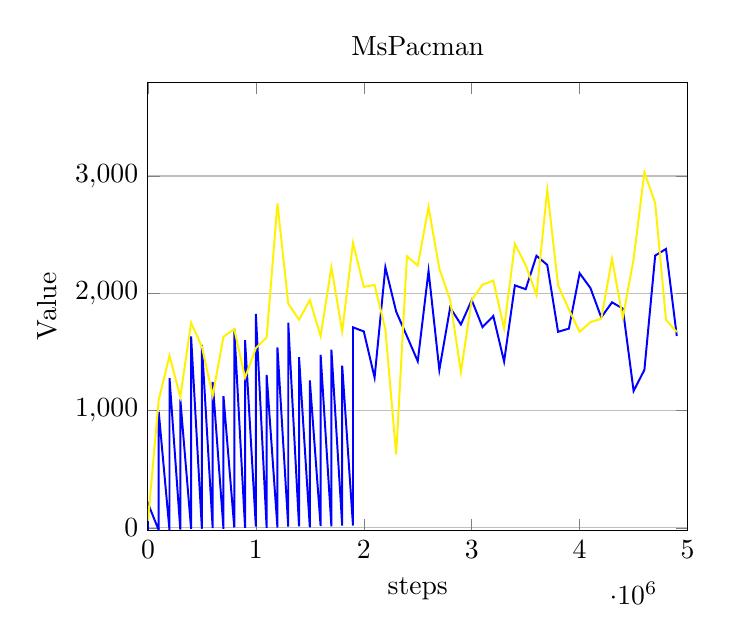
\begin{tikzpicture}

\begin{axis}[%
title=MsPacman,
% %width=4.634in,
%width=10in,
%height=5in,
%at={(2.596in,2.358in)},
% scale only axis,
xmin=0,
xmax=5000000,
xlabel style={font=\color{white!15!black}},
xlabel={steps},
xlabel near ticks,
ymin=-22,
ymax=3800,
ylabel style={font=\color{white!15!black}},
ylabel={Value},
ylabel near ticks,
ymajorgrids,
% %scale=0.5,
%scale=0.4,
axis background/.style={fill=white},
%legend style={legend cell align=left, align=left, draw=white!15!black}
]
\addplot [color=blue, line width = 0.25mm]
                table[row sep=crcr]{
                  0 -21.0\\ 
0 210.0\\ 
100000 -19.799999237060547\\ 
100000 990.0\\ 
200000 -20.700000762939453\\ 
200000 1277.0\\ 
300000 -15.0\\ 
300000 1096.0\\ 
400000 -7.0\\ 
400000 1632.0\\ 
500000 -6.900000095367432\\ 
500000 1561.0\\ 
600000 -1.899999976158142\\ 
600000 1245.0\\ 
700000 -7.599999904632568\\ 
700000 1123.0\\ 
800000 4.0\\ 
800000 1696.0\\ 
900000 1.5\\ 
900000 1600.0\\ 
1000000 11.300000190734863\\ 
1000000 1824.0\\ 
1100000 1.2000000476837158\\ 
1100000 1304.0\\ 
1200000 3.700000047683716\\ 
1200000 1538.0\\ 
1300000 11.5\\ 
1300000 1750.0\\ 
1400000 13.600000381469727\\ 
1400000 1456.0\\ 
1500000 5.699999809265137\\ 
1500000 1258.0\\ 
1600000 15.600000381469727\\ 
1600000 1476.0\\ 
1700000 13.5\\ 
1700000 1519.0\\ 
1800000 19.299999237060547\\ 
1800000 1383.0\\ 
1900000 20.799999237060547\\ 
1900000 1710.0\\ 
2000000 1675.0\\ 
2100000 1282.0\\ 
2200000 2222.0\\ 
2300000 1844.0\\ 
2400000 1634.0\\ 
2500000 1421.0\\ 
2600000 2191.0\\ 
2700000 1347.0\\ 
2800000 1878.0\\ 
2900000 1735.0\\ 
3000000 1942.0\\ 
3100000 1712.0\\ 
3200000 1806.0\\ 
3300000 1419.0\\ 
3400000 2068.0\\ 
3500000 2035.0\\ 
3600000 2320.0\\ 
3700000 2242.0\\ 
3800000 1672.0\\ 
3900000 1699.0\\ 
4000000 2171.0\\ 
4100000 2045.0\\ 
4200000 1795.0\\ 
4300000 1923.0\\ 
4400000 1870.0\\ 
4500000 1167.0\\ 
4600000 1348.0\\ 
4700000 2322.0\\ 
4800000 2378.0\\ 
4900000 1636.0\\ 
};
\addplot [color=red, line width = 0.25mm]
                table[row sep=crcr]{
                  0 0.0\\ 
};
\addplot [color=yellow, line width = 0.25mm]
                table[row sep=crcr]{
                  0 60.0\\ 
100000 1090.0\\ 
200000 1469.0\\ 
300000 1117.0\\ 
400000 1749.0\\ 
500000 1545.0\\ 
600000 1128.0\\ 
700000 1630.0\\ 
800000 1695.0\\ 
900000 1281.0\\ 
1000000 1532.0\\ 
1100000 1625.0\\ 
1200000 2767.0\\ 
1300000 1912.0\\ 
1400000 1775.0\\ 
1500000 1942.0\\ 
1600000 1636.0\\ 
1700000 2222.0\\ 
1800000 1676.0\\ 
1900000 2430.0\\ 
2000000 2055.0\\ 
2100000 2072.0\\ 
2200000 1693.0\\ 
2300000 625.0\\ 
2400000 2317.0\\ 
2500000 2236.0\\ 
2600000 2736.0\\ 
2700000 2209.0\\ 
2800000 1944.0\\ 
2900000 1329.0\\ 
3000000 1944.0\\ 
3100000 2074.0\\ 
3200000 2109.0\\ 
3300000 1701.0\\ 
3400000 2421.0\\ 
3500000 2240.0\\ 
3600000 1986.0\\ 
3700000 2883.0\\ 
3800000 2069.0\\ 
3900000 1863.0\\ 
4000000 1672.0\\ 
4100000 1754.0\\ 
4200000 1783.0\\ 
4300000 2293.0\\ 
4400000 1791.0\\ 
4500000 2293.0\\ 
4600000 3033.0\\ 
4700000 2768.0\\ 
4800000 1774.0\\ 
4900000 1670.0\\ 
};
\end{axis}
\end{tikzpicture}}}
    \subfloat[]{  \resizebox{0.4\textwidth}{!}{
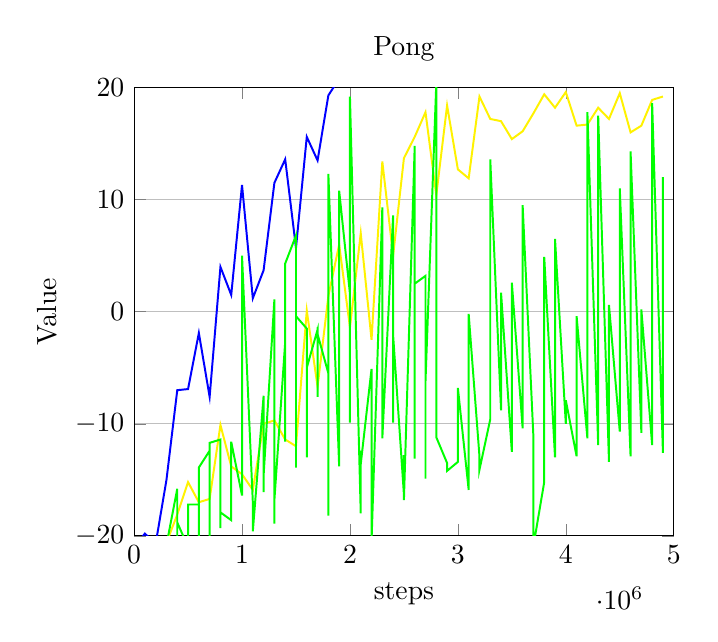
\begin{tikzpicture}

\begin{axis}[%
title=Pong,
% %width=4.634in,
%width=10in,
%height=5in,
%at={(2.596in,2.358in)},
% scale only axis,
xmin=0,
xmax=5000000,
xlabel style={font=\color{white!15!black}},
xlabel={steps},
xlabel near ticks,
ymin=-20,
ymax=20,
ylabel style={font=\color{white!15!black}},
ylabel={Value},
ylabel near ticks,
ymajorgrids,
% %scale=0.5,
%scale=0.4,
axis background/.style={fill=white},
%legend style={legend cell align=left, align=left, draw=white!15!black}
]
\addplot [color=blue, line width = 0.25mm]
                table[row sep=crcr]{
                  0 -21.0\\ 
100000 -19.799999237060547\\ 
200000 -20.700000762939453\\ 
300000 -15.0\\ 
400000 -7.0\\ 
500000 -6.900000095367432\\ 
600000 -1.899999976158142\\ 
700000 -7.599999904632568\\ 
800000 4.0\\ 
900000 1.5\\ 
1000000 11.300000190734863\\ 
1100000 1.2000000476837158\\ 
1200000 3.700000047683716\\ 
1300000 11.5\\ 
1400000 13.600000381469727\\ 
1500000 5.699999809265137\\ 
1600000 15.600000381469727\\ 
1700000 13.5\\ 
1800000 19.299999237060547\\ 
1900000 20.799999237060547\\ 
};
\addplot [color=red, line width = 0.25mm]
                table[row sep=crcr]{
                  0 0.0\\ 
};
\addplot [color=yellow, line width = 0.25mm]
                table[row sep=crcr]{
                  0 -21.0\\ 
0 -21.0\\ 
0 -21.0\\ 
100000 -21.0\\ 
200000 -20.299999237060547\\ 
300000 -20.600000381469727\\ 
400000 -18.100000381469727\\ 
500000 -15.199999809265137\\ 
600000 -17.0\\ 
700000 -16.700000762939453\\ 
800000 -10.100000381469727\\ 
900000 -13.800000190734863\\ 
1000000 -14.5\\ 
1100000 -15.899999618530273\\ 
1200000 -10.0\\ 
1300000 -9.699999809265137\\ 
1400000 -11.399999618530273\\ 
1500000 -12.0\\ 
1600000 0.10000000149011612\\ 
1700000 -6.699999809265137\\ 
1800000 1.399999976158142\\ 
1900000 6.0\\ 
2000000 -1.399999976158142\\ 
2100000 7.0\\ 
2200000 -2.5\\ 
2300000 13.399999618530273\\ 
2400000 5.0\\ 
2500000 13.699999809265137\\ 
2600000 15.600000381469727\\ 
2700000 17.799999237060547\\ 
2800000 10.399999618530273\\ 
2900000 18.399999618530273\\ 
3000000 12.699999809265137\\ 
3100000 11.899999618530273\\ 
3200000 19.200000762939453\\ 
3300000 17.200000762939453\\ 
3400000 17.0\\ 
3500000 15.399999618530273\\ 
3600000 16.100000381469727\\ 
3700000 17.700000762939453\\ 
3800000 19.399999618530273\\ 
3900000 18.200000762939453\\ 
4000000 19.600000381469727\\ 
4100000 16.600000381469727\\ 
4200000 16.700000762939453\\ 
4300000 18.200000762939453\\ 
4400000 17.200000762939453\\ 
4500000 19.5\\ 
4600000 16.0\\ 
4700000 16.600000381469727\\ 
4800000 18.899999618530273\\ 
4900000 19.200000762939453\\ 
};
\addplot [color=green, line width = 0.25mm]
                table[row sep=crcr]{
                  0 -21.0\\ 
0 -21.0\\ 
0 -21.0\\ 
0 -21.0\\ 
100000 -21.0\\ 
100000 -20.600000381469727\\ 
100000 -21.0\\ 
200000 -20.399999618530273\\ 
200000 -21.0\\ 
200000 -20.799999237060547\\ 
300000 -20.600000381469727\\ 
300000 -20.799999237060547\\ 
300000 -20.799999237060547\\ 
400000 -15.800000190734863\\ 
400000 -20.399999618530273\\ 
400000 -18.799999237060547\\ 
500000 -21.0\\ 
500000 -21.0\\ 
500000 -17.200000762939453\\ 
600000 -17.200000762939453\\ 
600000 -20.600000381469727\\ 
600000 -13.899999618530273\\ 
700000 -12.399999618530273\\ 
700000 -20.100000381469727\\ 
700000 -11.699999809265137\\ 
800000 -11.399999618530273\\ 
800000 -19.299999237060547\\ 
800000 -17.899999618530273\\ 
900000 -18.600000381469727\\ 
900000 -15.699999809265137\\ 
900000 -11.600000381469727\\ 
1000000 -16.399999618530273\\ 
1000000 -16.0\\ 
1000000 5.0\\ 
1100000 -17.0\\ 
1100000 -17.5\\ 
1100000 -19.600000381469727\\ 
1200000 -7.5\\ 
1200000 -16.100000381469727\\ 
1200000 -14.600000381469727\\ 
1300000 1.100000023841858\\ 
1300000 -18.899999618530273\\ 
1300000 -16.799999237060547\\ 
1400000 -2.700000047683716\\ 
1400000 -11.600000381469727\\ 
1400000 4.300000190734863\\ 
1500000 6.800000190734863\\ 
1500000 -13.899999618530273\\ 
1500000 -0.4000000059604645\\ 
1600000 -1.5\\ 
1600000 -13.0\\ 
1600000 -5.0\\ 
1700000 -1.600000023841858\\ 
1700000 -7.599999904632568\\ 
1700000 -2.0\\ 
1800000 -5.5\\ 
1800000 -18.200000762939453\\ 
1800000 12.300000190734863\\ 
1900000 -13.800000190734863\\ 
1900000 -10.0\\ 
1900000 10.800000190734863\\ 
2000000 1.600000023841858\\ 
2000000 -9.899999618530273\\ 
2000000 19.200000762939453\\ 
2100000 -18.0\\ 
2100000 -12.399999618530273\\ 
2100000 -13.600000381469727\\ 
2200000 -5.099999904632568\\ 
2200000 -13.899999618530273\\ 
2200000 -20.5\\ 
2300000 9.300000190734863\\ 
2300000 -8.199999809265137\\ 
2300000 -11.300000190734863\\ 
2400000 8.600000381469727\\ 
2400000 -9.899999618530273\\ 
2400000 -2.0999999046325684\\ 
2500000 -16.299999237060547\\ 
2500000 -12.800000190734863\\ 
2500000 -16.799999237060547\\ 
2600000 14.800000190734863\\ 
2600000 -13.100000381469727\\ 
2600000 2.5\\ 
2700000 3.200000047683716\\ 
2700000 -14.899999618530273\\ 
2700000 -6.199999809265137\\ 
2800000 20.399999618530273\\ 
2800000 -9.800000190734863\\ 
2800000 -11.199999809265137\\ 
2900000 -13.5\\ 
2900000 -14.199999809265137\\ 
3000000 -13.399999618530273\\ 
3000000 -6.800000190734863\\ 
3100000 -15.899999618530273\\ 
3100000 -0.20000000298023224\\ 
3200000 -12.899999618530273\\ 
3200000 -14.100000381469727\\ 
3300000 -9.600000381469727\\ 
3300000 13.600000381469727\\ 
3400000 -8.800000190734863\\ 
3400000 1.7000000476837158\\ 
3500000 -12.5\\ 
3500000 2.5999999046325684\\ 
3600000 -10.399999618530273\\ 
3600000 9.5\\ 
3700000 -11.199999809265137\\ 
3700000 -20.899999618530273\\ 
3800000 -15.199999809265137\\ 
3800000 4.900000095367432\\ 
3900000 -13.0\\ 
3900000 6.5\\ 
4000000 -10.0\\ 
4000000 -7.900000095367432\\ 
4100000 -12.899999618530273\\ 
4100000 -0.4000000059604645\\ 
4200000 -11.300000190734863\\ 
4200000 17.799999237060547\\ 
4300000 -11.899999618530273\\ 
4300000 17.5\\ 
4400000 -13.399999618530273\\ 
4400000 0.6000000238418579\\ 
4500000 -10.699999809265137\\ 
4500000 11.0\\ 
4600000 -12.899999618530273\\ 
4600000 14.300000190734863\\ 
4700000 -10.800000190734863\\ 
4700000 0.20000000298023224\\ 
4800000 -11.899999618530273\\ 
4800000 18.600000381469727\\ 
4900000 -12.600000381469727\\ 
4900000 12.0\\ 
};
\end{axis}
\end{tikzpicture}}}\\
    \ref{named}
%  \label{fig:rl-only-vs-pretrained}
\end{figure}
\end{frame}


\begin{frame}[plain]
		\centering
		\underline{Effectiveness of regularization --- continued}
		\vspace{-1cm}
\begin{figure}[!t]
  \captionsetup[subfloat]{position=top,labelformat=empty}
  \centering
    \subfloat[]{  \resizebox{0.4\textwidth}{!}{
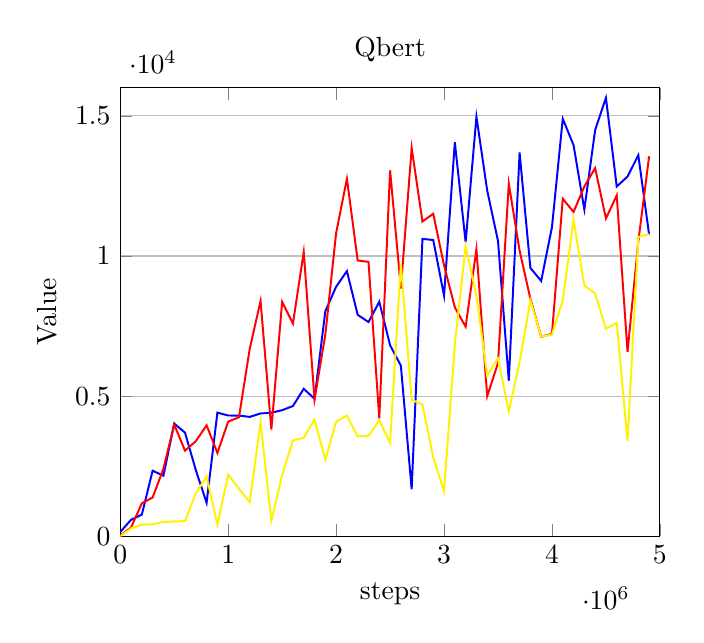
\begin{tikzpicture}

\begin{axis}[%
title=Qbert,
% %width=4.634in,
%width=10in,
%height=5in,
%at={(2.596in,2.358in)},
% scale only axis,
xmin=0,
xmax=5000000,
xlabel style={font=\color{white!15!black}},
xlabel={steps},
xlabel near ticks,
ymin=0,
ymax=16000,
ylabel style={font=\color{white!15!black}},
ylabel={Value},
ylabel near ticks,
ymajorgrids,
% %scale=0.5,
%scale=0.4,
axis background/.style={fill=white},
%legend style={legend cell align=left, align=left, draw=white!15!black}
]
\addplot [color=blue, line width = 0.25mm]
                table[row sep=crcr]{
                  0 150.0\\ 
100000 585.0\\ 
200000 772.5\\ 
300000 2337.5\\ 
400000 2157.5\\ 
500000 4022.5\\ 
600000 3695.0\\ 
700000 2362.5\\ 
800000 1192.5\\ 
900000 4410.0\\ 
1000000 4307.5\\ 
1100000 4305.0\\ 
1200000 4257.5\\ 
1300000 4380.0\\ 
1400000 4407.5\\ 
1500000 4497.5\\ 
1600000 4645.0\\ 
1700000 5260.0\\ 
1800000 4905.0\\ 
1900000 8030.0\\ 
2000000 8902.5\\ 
2100000 9460.0\\ 
2200000 7900.0\\ 
2300000 7642.5\\ 
2400000 8367.5\\ 
2500000 6815.0\\ 
2600000 6085.0\\ 
2700000 1677.5\\ 
2800000 10610.0\\ 
2900000 10570.0\\ 
3000000 8585.0\\ 
3100000 14057.5\\ 
3200000 10490.0\\ 
3300000 14970.0\\ 
3400000 12332.5\\ 
3500000 10537.5\\ 
3600000 5550.0\\ 
3700000 13692.5\\ 
3800000 9572.5\\ 
3900000 9110.0\\ 
4000000 11030.0\\ 
4100000 14897.5\\ 
4200000 13955.0\\ 
4300000 11660.0\\ 
4400000 14495.0\\ 
4500000 15645.0\\ 
4600000 12480.0\\ 
4700000 12835.0\\ 
4800000 13597.5\\ 
4900000 10762.5\\ 
};
\addplot [color=red, line width = 0.25mm]
                table[row sep=crcr]{
                  0 22.5\\ 
100000 310.0\\ 
200000 1172.5\\ 
300000 1382.5\\ 
400000 2410.0\\ 
500000 3982.5\\ 
600000 3052.5\\ 
700000 3390.0\\ 
800000 3957.5\\ 
900000 2970.0\\ 
1000000 4090.0\\ 
1100000 4245.0\\ 
1200000 6697.5\\ 
1300000 8395.0\\ 
1400000 3807.5\\ 
1500000 8360.0\\ 
1600000 7590.0\\ 
1700000 10142.5\\ 
1800000 4877.5\\ 
1900000 7190.0\\ 
2000000 10817.5\\ 
2100000 12755.0\\ 
2200000 9840.0\\ 
2300000 9790.0\\ 
2400000 4202.5\\ 
2500000 13057.5\\ 
2600000 8842.5\\ 
2700000 13852.5\\ 
2800000 11230.0\\ 
2900000 11507.5\\ 
3000000 9665.0\\ 
3100000 8167.5\\ 
3200000 7475.0\\ 
3300000 10242.5\\ 
3400000 4997.5\\ 
3500000 6180.0\\ 
3600000 12582.5\\ 
3700000 10190.0\\ 
3800000 8475.0\\ 
3900000 7115.0\\ 
4000000 7222.5\\ 
4100000 12042.5\\ 
4200000 11572.5\\ 
4300000 12480.0\\ 
4400000 13137.5\\ 
4500000 11337.5\\ 
4600000 12165.0\\ 
4700000 6580.0\\ 
4800000 10517.5\\ 
4900000 13560.0\\ 
};
\addplot [color=yellow, line width = 0.25mm]
                table[row sep=crcr]{
                  0 0.0\\ 
100000 280.0\\ 
200000 415.0\\ 
300000 425.0\\ 
400000 507.5\\ 
500000 525.0\\ 
600000 537.5\\ 
700000 1525.0\\ 
800000 2137.5\\ 
900000 407.5\\ 
1000000 2195.0\\ 
1100000 1690.0\\ 
1200000 1215.0\\ 
1300000 4077.5\\ 
1400000 550.0\\ 
1500000 2185.0\\ 
1600000 3417.5\\ 
1700000 3512.5\\ 
1800000 4165.0\\ 
1900000 2730.0\\ 
2000000 4090.0\\ 
2100000 4305.0\\ 
2200000 3557.5\\ 
2300000 3585.0\\ 
2400000 4137.5\\ 
2500000 3335.0\\ 
2600000 9722.5\\ 
2700000 4865.0\\ 
2800000 4700.0\\ 
2900000 2812.5\\ 
3000000 1605.0\\ 
3100000 6847.5\\ 
3200000 10342.5\\ 
3300000 8590.0\\ 
3400000 5732.5\\ 
3500000 6345.0\\ 
3600000 4447.5\\ 
3700000 6217.5\\ 
3800000 8415.0\\ 
3900000 7120.0\\ 
4000000 7195.0\\ 
4100000 8415.0\\ 
4200000 11307.5\\ 
4300000 8942.5\\ 
4400000 8662.5\\ 
4500000 7402.5\\ 
4600000 7612.5\\ 
4700000 3395.0\\ 
4800000 10680.0\\ 
4900000 10780.0\\ 
};
\end{axis}
\end{tikzpicture}}}
    \subfloat[]{  \resizebox{0.4\textwidth}{!}{
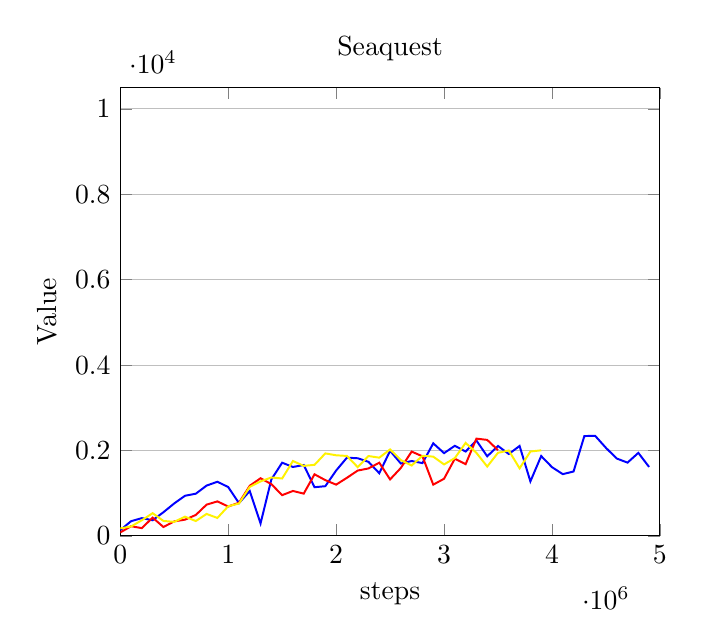
\begin{tikzpicture}

\begin{axis}[%
title=Seaquest,
% %width=4.634in,
%width=10in,
%height=5in,
%at={(2.596in,2.358in)},
% scale only axis,
xmin=0,
xmax=5000000,
xlabel style={font=\color{white!15!black}},
xlabel={steps},
xlabel near ticks,
ymin=0,
ymax=10500,
ylabel style={font=\color{white!15!black}},
ylabel={Value},
ylabel near ticks,
ymajorgrids,
% %scale=0.5,
%scale=0.4,
axis background/.style={fill=white},
%legend style={legend cell align=left, align=left, draw=white!15!black}
]
\addplot [color=blue, line width = 0.25mm]
                table[row sep=crcr]{
                  0 134.0\\ 
100000 344.0\\ 
200000 416.0\\ 
300000 366.0\\ 
400000 554.0\\ 
500000 760.0\\ 
600000 940.0\\ 
700000 988.0\\ 
800000 1178.0\\ 
900000 1268.0\\ 
1000000 1144.0\\ 
1100000 768.0\\ 
1200000 1052.0\\ 
1300000 292.0\\ 
1400000 1322.0\\ 
1500000 1714.0\\ 
1600000 1614.0\\ 
1700000 1660.0\\ 
1800000 1140.0\\ 
1900000 1164.0\\ 
2000000 1530.0\\ 
2100000 1832.0\\ 
2200000 1818.0\\ 
2300000 1734.0\\ 
2400000 1468.0\\ 
2500000 1992.0\\ 
2600000 1694.0\\ 
2700000 1754.0\\ 
2800000 1704.0\\ 
2900000 2168.0\\ 
3000000 1938.0\\ 
3100000 2110.0\\ 
3200000 1976.0\\ 
3300000 2234.0\\ 
3400000 1864.0\\ 
3500000 2106.0\\ 
3600000 1918.0\\ 
3700000 2106.0\\ 
3800000 1276.0\\ 
3900000 1870.0\\ 
4000000 1610.0\\ 
4100000 1446.0\\ 
4200000 1508.0\\ 
4300000 2338.0\\ 
4400000 2344.0\\ 
4500000 2062.0\\ 
4600000 1812.0\\ 
4700000 1716.0\\ 
4800000 1944.0\\ 
4900000 1614.0\\ 
};
\addplot [color=red, line width = 0.25mm]
                table[row sep=crcr]{
                  0 80.0\\ 
100000 226.0\\ 
200000 182.0\\ 
300000 428.0\\ 
400000 208.0\\ 
500000 340.0\\ 
600000 380.0\\ 
700000 490.0\\ 
800000 732.0\\ 
900000 808.0\\ 
1000000 688.0\\ 
1100000 776.0\\ 
1200000 1174.0\\ 
1300000 1350.0\\ 
1400000 1212.0\\ 
1500000 954.0\\ 
1600000 1052.0\\ 
1700000 990.0\\ 
1800000 1442.0\\ 
1900000 1306.0\\ 
2000000 1200.0\\ 
2100000 1360.0\\ 
2200000 1530.0\\ 
2300000 1580.0\\ 
2400000 1714.0\\ 
2500000 1322.0\\ 
2600000 1592.0\\ 
2700000 1974.0\\ 
2800000 1864.0\\ 
2900000 1200.0\\ 
3000000 1338.0\\ 
3100000 1808.0\\ 
3200000 1680.0\\ 
3300000 2278.0\\ 
3400000 2248.0\\ 
3500000 2008.0\\ 
};
\addplot [color=yellow, line width = 0.25mm]
                table[row sep=crcr]{
                  0 176.0\\ 
100000 220.0\\ 
200000 366.0\\ 
300000 532.0\\ 
400000 350.0\\ 
500000 328.0\\ 
600000 450.0\\ 
700000 348.0\\ 
800000 514.0\\ 
900000 420.0\\ 
1000000 694.0\\ 
1100000 758.0\\ 
1200000 1148.0\\ 
1300000 1276.0\\ 
1400000 1368.0\\ 
1500000 1344.0\\ 
1600000 1754.0\\ 
1700000 1640.0\\ 
1800000 1664.0\\ 
1900000 1932.0\\ 
2000000 1888.0\\ 
2100000 1872.0\\ 
2200000 1610.0\\ 
2300000 1870.0\\ 
2400000 1832.0\\ 
2500000 2024.0\\ 
2600000 1774.0\\ 
2700000 1648.0\\ 
2800000 1876.0\\ 
2900000 1856.0\\ 
3000000 1674.0\\ 
3100000 1822.0\\ 
3200000 2178.0\\ 
3300000 1944.0\\ 
3400000 1624.0\\ 
3500000 1946.0\\ 
3600000 2000.0\\ 
3700000 1582.0\\ 
3800000 1976.0\\ 
3900000 2004.0\\ 
};
\end{axis}
\end{tikzpicture}}}\\
  \vspace{-1cm}
    \subfloat[]{  \resizebox{0.4\textwidth}{!}{
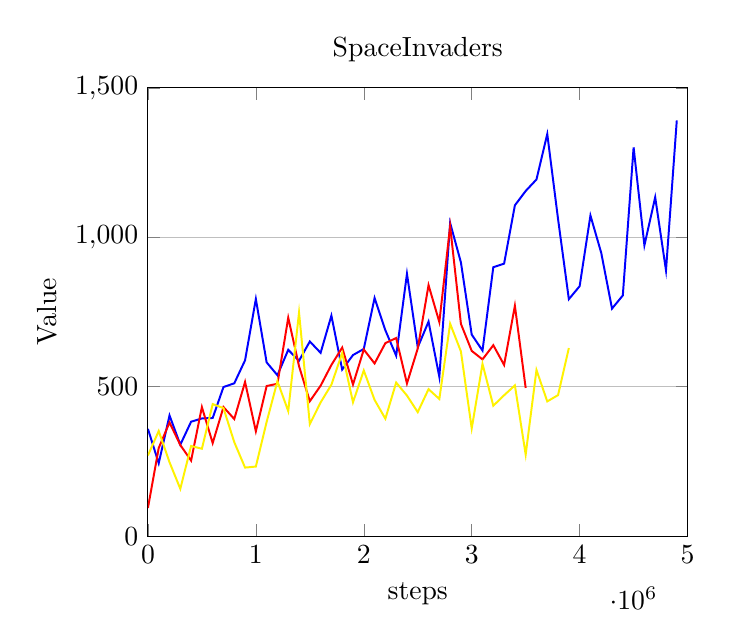
\begin{tikzpicture}

\begin{axis}[%
title=SpaceInvaders,
%width=10in,
%height=5in,
%at={(2.596in,2.358in)},
% scale only axis,
xmin=0,
xmax=5000000,
xlabel style={font=\color{white!15!black}},
xlabel={steps},
xlabel near ticks,
ymin=0,
ymax=1500,
ylabel style={font=\color{white!15!black}},
ylabel={Value},
ylabel near ticks,
ymajorgrids,
% %scale=0.5,
%scale=0.4,
axis background/.style={fill=white},
%legend style={legend cell align=left, align=left, draw=white!15!black}
]
\addplot [color=blue, line width = 0.25mm]
                table[row sep=crcr]{
                  0 359.0\\ 
100000 244.0\\ 
200000 404.0\\ 
300000 306.0\\ 
400000 383.0\\ 
500000 394.0\\ 
600000 395.5\\ 
700000 499.0\\ 
800000 511.5\\ 
900000 588.5\\ 
1000000 793.5\\ 
1100000 581.5\\ 
1200000 538.5\\ 
1300000 623.5\\ 
1400000 587.0\\ 
1500000 651.5\\ 
1600000 613.5\\ 
1700000 738.0\\ 
1800000 557.5\\ 
1900000 606.0\\ 
2000000 626.5\\ 
2100000 797.0\\ 
2200000 689.0\\ 
2300000 604.0\\ 
2400000 878.0\\ 
2500000 632.0\\ 
2600000 718.0\\ 
2700000 533.0\\ 
2800000 1048.0\\ 
2900000 916.0\\ 
3000000 674.5\\ 
3100000 621.0\\ 
3200000 900.0\\ 
3300000 912.0\\ 
3400000 1107.0\\ 
3500000 1155.0\\ 
3600000 1193.5\\ 
3700000 1345.5\\ 
3800000 1061.0\\ 
3900000 793.0\\ 
4000000 836.5\\ 
4100000 1073.0\\ 
4200000 948.0\\ 
4300000 761.5\\ 
4400000 805.5\\ 
4500000 1301.0\\ 
4600000 973.0\\ 
4700000 1134.0\\ 
4800000 889.5\\ 
4900000 1391.0\\ 
};
\addplot [color=red, line width = 0.25mm]
                table[row sep=crcr]{
                  0 94.5\\ 
100000 295.0\\ 
200000 380.5\\ 
300000 305.0\\ 
400000 253.0\\ 
500000 432.0\\ 
600000 311.5\\ 
700000 432.0\\ 
800000 392.0\\ 
900000 516.0\\ 
1000000 351.0\\ 
1100000 502.5\\ 
1200000 510.0\\ 
1300000 731.0\\ 
1400000 569.0\\ 
1500000 451.5\\ 
1600000 503.5\\ 
1700000 573.0\\ 
1800000 631.0\\ 
1900000 507.5\\ 
2000000 624.5\\ 
2100000 578.0\\ 
2200000 646.0\\ 
2300000 663.0\\ 
2400000 511.0\\ 
2500000 628.0\\ 
2600000 840.0\\ 
2700000 716.5\\ 
2800000 1037.0\\ 
2900000 710.5\\ 
3000000 620.0\\ 
3100000 591.5\\ 
3200000 639.0\\ 
3300000 573.0\\ 
3400000 771.0\\ 
3500000 496.0\\ 
};
\addplot [color=yellow, line width = 0.25mm]
                table[row sep=crcr]{
                  0 270.0\\ 
100000 352.0\\ 
200000 247.5\\ 
300000 158.5\\ 
400000 302.0\\ 
500000 292.5\\ 
600000 442.0\\ 
700000 428.5\\ 
800000 314.5\\ 
900000 229.5\\ 
1000000 233.0\\ 
1100000 382.5\\ 
1200000 518.5\\ 
1300000 418.5\\ 
1400000 748.5\\ 
1500000 375.0\\ 
1600000 447.5\\ 
1700000 507.0\\ 
1800000 613.0\\ 
1900000 448.0\\ 
2000000 554.5\\ 
2100000 456.0\\ 
2200000 393.0\\ 
2300000 514.0\\ 
2400000 470.5\\ 
2500000 415.0\\ 
2600000 492.0\\ 
2700000 459.0\\ 
2800000 711.0\\ 
2900000 618.0\\ 
3000000 360.5\\ 
3100000 576.5\\ 
3200000 436.5\\ 
3300000 471.5\\ 
3400000 504.5\\ 
3500000 273.0\\ 
3600000 556.0\\ 
3700000 451.0\\ 
3800000 472.0\\ 
3900000 629.5\\ 
};
\end{axis}
\end{tikzpicture}}}
  \\
    \ref{named}
\end{figure}
\end{frame}


\begin{frame}[plain]
		\centering
		\underline{Effectiveness of predicting}
		\vspace{-1cm}
\begin{figure}[!t]
  \captionsetup[subfloat]{position=top,labelformat=empty}
  \centering
    \subfloat[]{  \resizebox{0.4\textwidth}{!}{
%\definecolor{blue}{RGB}{76,100,135}
%\definecolor{red}{RGB}{153,0,0}
%\definecolor{yellow}{RGB}{227,178,60}
%\definecolor{mycolor1}{rgb}{0.00000,0.44700,0.74100}%
%\definecolor{mycolor2}{rgb}{0.85000,0.32500,0.09800}%
%\definecolor{mycolor3}{rgb}{0.92900,0.69400,0.12500}%
%
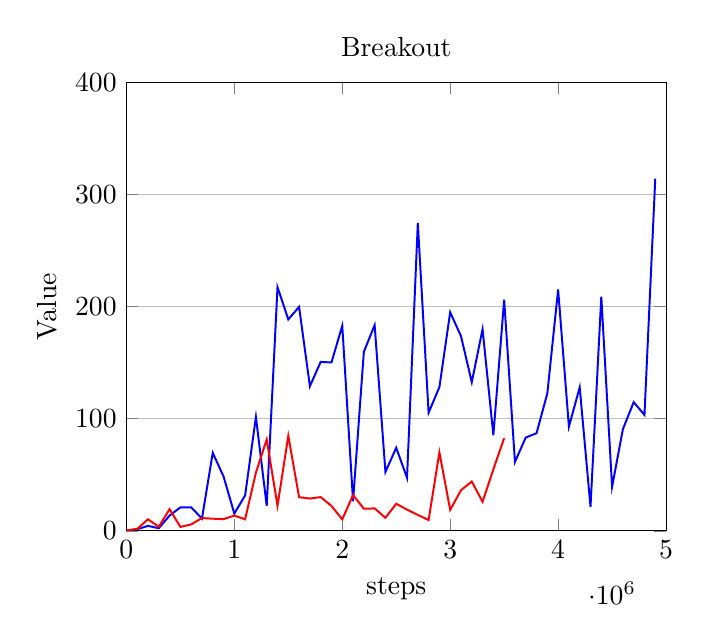
\begin{tikzpicture}

\begin{axis}[%
legend entries={rl-only-small-net,L2-reg,parallel-fs-50-no-aug}, 
legend columns=2,
title=Breakout,
legend to name=named,
legend style={legend cell align=left},
%%width=10in,
%%height=5in,
%%at={(2.596in,2.358in)},
% scale only axis,
xmin=0,
xmax=5000000,
xlabel style={font=\color{white!15!black}},
xlabel={steps},
xlabel near ticks,
ymin=0,
ymax=400,
ylabel style={font=\color{white!15!black}},
ylabel={Value},
ylabel near ticks,
ymajorgrids,
% %scale=0.5,
%%scale=0.4,
axis background/.style={fill=white},
%legend columns=2,
%legend=south outside
]
\addplot [color=blue, line width = 0.25mm]
                table[row sep=crcr]{
                  0 0.20000000298023224\\ 
100000 1.399999976158142\\ 
200000 4.400000095367432\\ 
300000 2.299999952316284\\ 
400000 13.600000381469727\\ 
500000 20.899999618530273\\ 
600000 21.0\\ 
700000 10.899999618530273\\ 
800000 69.5999984741211\\ 
900000 48.5\\ 
1000000 15.399999618530273\\ 
1100000 31.600000381469727\\ 
1200000 101.5999984741211\\ 
1300000 22.399999618530273\\ 
1400000 217.39999389648438\\ 
1500000 188.60000610351562\\ 
1600000 199.8000030517578\\ 
1700000 129.0\\ 
1800000 150.6999969482422\\ 
1900000 150.1999969482422\\ 
2000000 183.0\\ 
2100000 26.399999618530273\\ 
2200000 159.6999969482422\\ 
2300000 183.5\\ 
2400000 52.5\\ 
2500000 74.0999984741211\\ 
2600000 47.29999923706055\\ 
2700000 274.6000061035156\\ 
2800000 105.4000015258789\\ 
2900000 128.1999969482422\\ 
3000000 195.0\\ 
3100000 173.6999969482422\\ 
3200000 132.60000610351562\\ 
3300000 179.89999389648438\\ 
3400000 85.19999694824219\\ 
3500000 206.1999969482422\\ 
3600000 61.5\\ 
3700000 83.19999694824219\\ 
3800000 87.0999984741211\\ 
3900000 122.5999984741211\\ 
4000000 215.3000030517578\\ 
4100000 92.9000015258789\\ 
4200000 128.0\\ 
4300000 21.399999618530273\\ 
4400000 208.89999389648438\\ 
4500000 39.20000076293945\\ 
4600000 90.5999984741211\\ 
4700000 114.80000305175781\\ 
4800000 103.4000015258789\\ 
4900000 314.20001220703125\\ 
};
\addplot [color=red, line width = 0.25mm]
                table[row sep=crcr]{
                  0 0.4000000059604645\\ 
100000 1.7000000476837158\\ 
200000 10.300000190734863\\ 
300000 3.5999999046325684\\ 
400000 19.299999237060547\\ 
500000 3.5\\ 
600000 5.699999809265137\\ 
700000 11.399999618530273\\ 
800000 10.800000190734863\\ 
900000 10.399999618530273\\ 
1000000 13.600000381469727\\ 
1100000 10.300000190734863\\ 
1200000 51.900001525878906\\ 
1300000 81.5\\ 
1400000 22.299999237060547\\ 
1500000 84.69999694824219\\ 
1600000 30.0\\ 
1700000 28.799999237060547\\ 
1800000 30.100000381469727\\ 
1900000 22.200000762939453\\ 
2000000 10.199999809265137\\ 
2100000 31.899999618530273\\ 
2200000 19.700000762939453\\ 
2300000 20.0\\ 
2400000 11.600000381469727\\ 
2500000 24.200000762939453\\ 
2600000 18.899999618530273\\ 
2700000 14.199999809265137\\ 
2800000 9.600000381469727\\ 
2900000 70.0\\ 
3000000 18.700000762939453\\ 
3100000 36.20000076293945\\ 
3200000 44.0\\ 
3300000 25.899999618530273\\ 
3400000 54.900001525878906\\ 
3500000 82.69999694824219\\ 
};
\addplot [color=yellow, line width = 0.25mm]
                table[row sep=crcr]{
                  0 0.800000011920929\\ 
};
\end{axis}
\end{tikzpicture}}}
    \subfloat[]{  \resizebox{0.4\textwidth}{!}{
%\definecolor{blue}{RGB}{76,100,135}
%\definecolor{red}{RGB}{153,0,0}
%\definecolor{yellow}{RGB}{227,178,60}
%\definecolor{mycolor1}{rgb}{0.00000,0.44700,0.74100}%
%\definecolor{mycolor2}{rgb}{0.85000,0.32500,0.09800}%
%\definecolor{mycolor3}{rgb}{0.92900,0.69400,0.12500}%
%
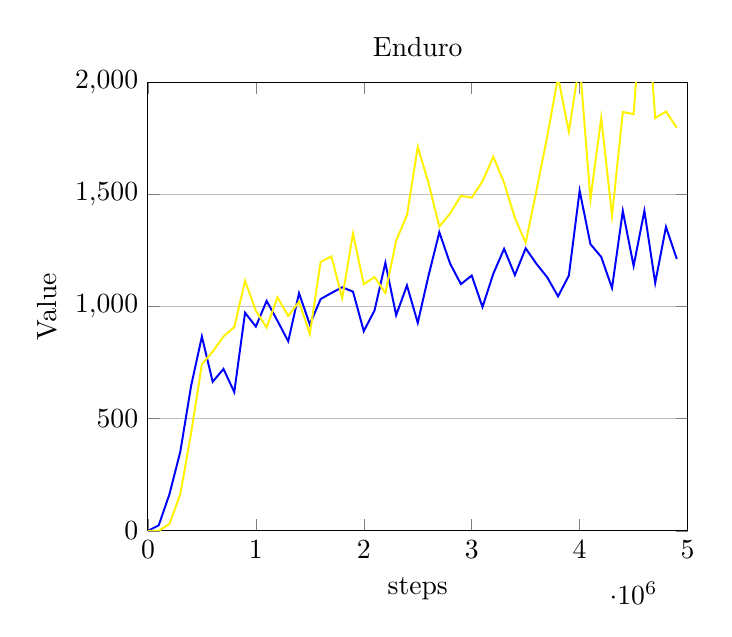
\begin{tikzpicture}

\begin{axis}[%
title=Enduro,
% %width=4.634in,
%%width=10in,
%%height=5in,
%at={(2.596in,2.358in)},
% scale only axis,
xmin=0,
xmax=5000000,
xlabel style={font=\color{white!15!black}},
xlabel={steps},
xlabel near ticks,
ymin=0,
ymax=2000,
ylabel style={font=\color{white!15!black}},
ylabel={Value},
ylabel near ticks,
ymajorgrids,
% %scale=0.5,
%scale=0.4,
axis background/.style={fill=white},
%legend style={legend cell align=left, align=left, draw=white!15!black}
]
\addplot [color=blue, line width = 0.25mm]
                table[row sep=crcr]{
                  0 0.0\\ 
100000 24.299999237060547\\ 
200000 164.3000030517578\\ 
300000 353.0\\ 
400000 646.4000244140625\\ 
500000 866.7000122070312\\ 
600000 664.7000122070312\\ 
700000 722.2000122070312\\ 
800000 618.9000244140625\\ 
900000 972.7999877929688\\ 
1000000 910.9000244140625\\ 
1100000 1025.699951171875\\ 
1200000 937.0\\ 
1300000 845.5999755859375\\ 
1400000 1059.9000244140625\\ 
1500000 920.2999877929688\\ 
1600000 1033.800048828125\\ 
1700000 1061.0\\ 
1800000 1086.5999755859375\\ 
1900000 1066.9000244140625\\ 
2000000 890.9000244140625\\ 
2100000 983.5\\ 
2200000 1195.300048828125\\ 
2300000 962.0\\ 
2400000 1094.800048828125\\ 
2500000 928.0\\ 
2600000 1138.5999755859375\\ 
2700000 1332.300048828125\\ 
2800000 1191.800048828125\\ 
2900000 1100.5999755859375\\ 
3000000 1138.800048828125\\ 
3100000 998.2999877929688\\ 
3200000 1146.800048828125\\ 
3300000 1258.0999755859375\\ 
3400000 1141.0\\ 
3500000 1260.300048828125\\ 
3600000 1190.800048828125\\ 
3700000 1130.5999755859375\\ 
3800000 1046.0999755859375\\ 
3900000 1138.4000244140625\\ 
4000000 1517.5\\ 
4100000 1278.9000244140625\\ 
4200000 1221.699951171875\\ 
4300000 1083.199951171875\\ 
4400000 1426.9000244140625\\ 
4500000 1181.5999755859375\\ 
4600000 1427.199951171875\\ 
4700000 1105.800048828125\\ 
4800000 1355.800048828125\\ 
4900000 1212.9000244140625\\ 
};
\addplot [color=red, line width = 0.25mm]
                table[row sep=crcr]{
                  0 0.0\\ 
};
\addplot [color=yellow, line width = 0.25mm]
                table[row sep=crcr]{
                  0 0.0\\ 
100000 0.0\\ 
200000 30.700000762939453\\ 
300000 163.6999969482422\\ 
400000 435.79998779296875\\ 
500000 743.2000122070312\\ 
600000 799.2000122070312\\ 
700000 867.0\\ 
800000 908.4000244140625\\ 
900000 1115.300048828125\\ 
1000000 981.4000244140625\\ 
1100000 906.9000244140625\\ 
1200000 1041.5999755859375\\ 
1300000 958.5999755859375\\ 
1400000 1021.9000244140625\\ 
1500000 877.7000122070312\\ 
1600000 1199.4000244140625\\ 
1700000 1224.0\\ 
1800000 1038.199951171875\\ 
1900000 1326.0999755859375\\ 
2000000 1100.0\\ 
2100000 1132.0999755859375\\ 
2200000 1060.9000244140625\\ 
2300000 1294.300048828125\\ 
2400000 1407.699951171875\\ 
2500000 1712.5\\ 
2600000 1551.5\\ 
2700000 1357.0\\ 
2800000 1415.800048828125\\ 
2900000 1494.5\\ 
3000000 1486.0\\ 
3100000 1559.699951171875\\ 
3200000 1668.5\\ 
3300000 1552.800048828125\\ 
3400000 1395.800048828125\\ 
3500000 1284.9000244140625\\ 
3600000 1518.0\\ 
3700000 1759.5999755859375\\ 
3800000 2024.9000244140625\\ 
3900000 1780.0999755859375\\ 
4000000 2090.5\\ 
4100000 1479.0999755859375\\ 
4200000 1841.699951171875\\ 
4300000 1405.5999755859375\\ 
4400000 1868.300048828125\\ 
4500000 1858.699951171875\\ 
4600000 2527.0\\ 
4700000 1841.0\\ 
4800000 1870.800048828125\\ 
4900000 1797.9000244140625\\ 
};
\end{axis}
\end{tikzpicture}}}\\
  \vspace{-1cm}
    \subfloat[]{  \resizebox{0.4\textwidth}{!}{
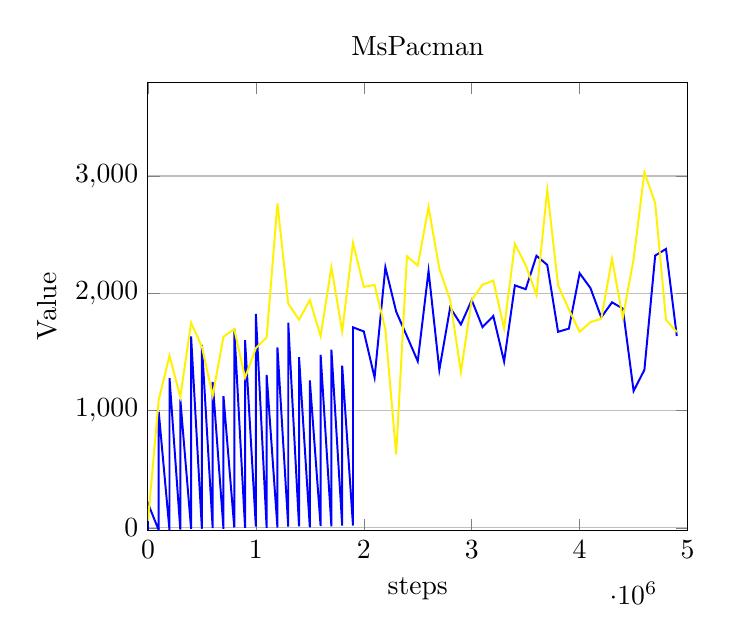
\begin{tikzpicture}

\begin{axis}[%
title=MsPacman,
% %width=4.634in,
%width=10in,
%height=5in,
%at={(2.596in,2.358in)},
% scale only axis,
xmin=0,
xmax=5000000,
xlabel style={font=\color{white!15!black}},
xlabel={steps},
xlabel near ticks,
ymin=-22,
ymax=3800,
ylabel style={font=\color{white!15!black}},
ylabel={Value},
ylabel near ticks,
ymajorgrids,
% %scale=0.5,
%scale=0.4,
axis background/.style={fill=white},
%legend style={legend cell align=left, align=left, draw=white!15!black}
]
\addplot [color=blue, line width = 0.25mm]
                table[row sep=crcr]{
                  0 -21.0\\ 
0 210.0\\ 
100000 -19.799999237060547\\ 
100000 990.0\\ 
200000 -20.700000762939453\\ 
200000 1277.0\\ 
300000 -15.0\\ 
300000 1096.0\\ 
400000 -7.0\\ 
400000 1632.0\\ 
500000 -6.900000095367432\\ 
500000 1561.0\\ 
600000 -1.899999976158142\\ 
600000 1245.0\\ 
700000 -7.599999904632568\\ 
700000 1123.0\\ 
800000 4.0\\ 
800000 1696.0\\ 
900000 1.5\\ 
900000 1600.0\\ 
1000000 11.300000190734863\\ 
1000000 1824.0\\ 
1100000 1.2000000476837158\\ 
1100000 1304.0\\ 
1200000 3.700000047683716\\ 
1200000 1538.0\\ 
1300000 11.5\\ 
1300000 1750.0\\ 
1400000 13.600000381469727\\ 
1400000 1456.0\\ 
1500000 5.699999809265137\\ 
1500000 1258.0\\ 
1600000 15.600000381469727\\ 
1600000 1476.0\\ 
1700000 13.5\\ 
1700000 1519.0\\ 
1800000 19.299999237060547\\ 
1800000 1383.0\\ 
1900000 20.799999237060547\\ 
1900000 1710.0\\ 
2000000 1675.0\\ 
2100000 1282.0\\ 
2200000 2222.0\\ 
2300000 1844.0\\ 
2400000 1634.0\\ 
2500000 1421.0\\ 
2600000 2191.0\\ 
2700000 1347.0\\ 
2800000 1878.0\\ 
2900000 1735.0\\ 
3000000 1942.0\\ 
3100000 1712.0\\ 
3200000 1806.0\\ 
3300000 1419.0\\ 
3400000 2068.0\\ 
3500000 2035.0\\ 
3600000 2320.0\\ 
3700000 2242.0\\ 
3800000 1672.0\\ 
3900000 1699.0\\ 
4000000 2171.0\\ 
4100000 2045.0\\ 
4200000 1795.0\\ 
4300000 1923.0\\ 
4400000 1870.0\\ 
4500000 1167.0\\ 
4600000 1348.0\\ 
4700000 2322.0\\ 
4800000 2378.0\\ 
4900000 1636.0\\ 
};
\addplot [color=red, line width = 0.25mm]
                table[row sep=crcr]{
                  0 0.0\\ 
};
\addplot [color=yellow, line width = 0.25mm]
                table[row sep=crcr]{
                  0 60.0\\ 
100000 1090.0\\ 
200000 1469.0\\ 
300000 1117.0\\ 
400000 1749.0\\ 
500000 1545.0\\ 
600000 1128.0\\ 
700000 1630.0\\ 
800000 1695.0\\ 
900000 1281.0\\ 
1000000 1532.0\\ 
1100000 1625.0\\ 
1200000 2767.0\\ 
1300000 1912.0\\ 
1400000 1775.0\\ 
1500000 1942.0\\ 
1600000 1636.0\\ 
1700000 2222.0\\ 
1800000 1676.0\\ 
1900000 2430.0\\ 
2000000 2055.0\\ 
2100000 2072.0\\ 
2200000 1693.0\\ 
2300000 625.0\\ 
2400000 2317.0\\ 
2500000 2236.0\\ 
2600000 2736.0\\ 
2700000 2209.0\\ 
2800000 1944.0\\ 
2900000 1329.0\\ 
3000000 1944.0\\ 
3100000 2074.0\\ 
3200000 2109.0\\ 
3300000 1701.0\\ 
3400000 2421.0\\ 
3500000 2240.0\\ 
3600000 1986.0\\ 
3700000 2883.0\\ 
3800000 2069.0\\ 
3900000 1863.0\\ 
4000000 1672.0\\ 
4100000 1754.0\\ 
4200000 1783.0\\ 
4300000 2293.0\\ 
4400000 1791.0\\ 
4500000 2293.0\\ 
4600000 3033.0\\ 
4700000 2768.0\\ 
4800000 1774.0\\ 
4900000 1670.0\\ 
};
\end{axis}
\end{tikzpicture}}}
    \subfloat[]{  \resizebox{0.4\textwidth}{!}{
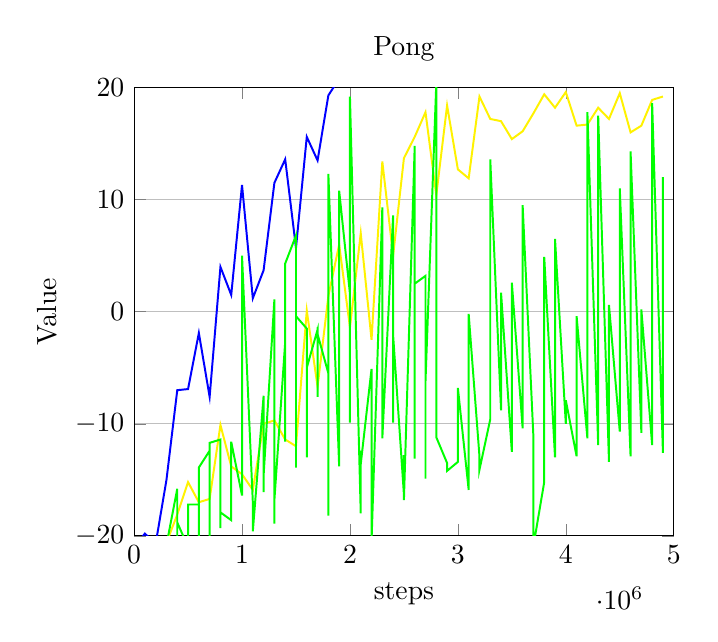
\begin{tikzpicture}

\begin{axis}[%
title=Pong,
% %width=4.634in,
%width=10in,
%height=5in,
%at={(2.596in,2.358in)},
% scale only axis,
xmin=0,
xmax=5000000,
xlabel style={font=\color{white!15!black}},
xlabel={steps},
xlabel near ticks,
ymin=-20,
ymax=20,
ylabel style={font=\color{white!15!black}},
ylabel={Value},
ylabel near ticks,
ymajorgrids,
% %scale=0.5,
%scale=0.4,
axis background/.style={fill=white},
%legend style={legend cell align=left, align=left, draw=white!15!black}
]
\addplot [color=blue, line width = 0.25mm]
                table[row sep=crcr]{
                  0 -21.0\\ 
100000 -19.799999237060547\\ 
200000 -20.700000762939453\\ 
300000 -15.0\\ 
400000 -7.0\\ 
500000 -6.900000095367432\\ 
600000 -1.899999976158142\\ 
700000 -7.599999904632568\\ 
800000 4.0\\ 
900000 1.5\\ 
1000000 11.300000190734863\\ 
1100000 1.2000000476837158\\ 
1200000 3.700000047683716\\ 
1300000 11.5\\ 
1400000 13.600000381469727\\ 
1500000 5.699999809265137\\ 
1600000 15.600000381469727\\ 
1700000 13.5\\ 
1800000 19.299999237060547\\ 
1900000 20.799999237060547\\ 
};
\addplot [color=red, line width = 0.25mm]
                table[row sep=crcr]{
                  0 0.0\\ 
};
\addplot [color=yellow, line width = 0.25mm]
                table[row sep=crcr]{
                  0 -21.0\\ 
0 -21.0\\ 
0 -21.0\\ 
100000 -21.0\\ 
200000 -20.299999237060547\\ 
300000 -20.600000381469727\\ 
400000 -18.100000381469727\\ 
500000 -15.199999809265137\\ 
600000 -17.0\\ 
700000 -16.700000762939453\\ 
800000 -10.100000381469727\\ 
900000 -13.800000190734863\\ 
1000000 -14.5\\ 
1100000 -15.899999618530273\\ 
1200000 -10.0\\ 
1300000 -9.699999809265137\\ 
1400000 -11.399999618530273\\ 
1500000 -12.0\\ 
1600000 0.10000000149011612\\ 
1700000 -6.699999809265137\\ 
1800000 1.399999976158142\\ 
1900000 6.0\\ 
2000000 -1.399999976158142\\ 
2100000 7.0\\ 
2200000 -2.5\\ 
2300000 13.399999618530273\\ 
2400000 5.0\\ 
2500000 13.699999809265137\\ 
2600000 15.600000381469727\\ 
2700000 17.799999237060547\\ 
2800000 10.399999618530273\\ 
2900000 18.399999618530273\\ 
3000000 12.699999809265137\\ 
3100000 11.899999618530273\\ 
3200000 19.200000762939453\\ 
3300000 17.200000762939453\\ 
3400000 17.0\\ 
3500000 15.399999618530273\\ 
3600000 16.100000381469727\\ 
3700000 17.700000762939453\\ 
3800000 19.399999618530273\\ 
3900000 18.200000762939453\\ 
4000000 19.600000381469727\\ 
4100000 16.600000381469727\\ 
4200000 16.700000762939453\\ 
4300000 18.200000762939453\\ 
4400000 17.200000762939453\\ 
4500000 19.5\\ 
4600000 16.0\\ 
4700000 16.600000381469727\\ 
4800000 18.899999618530273\\ 
4900000 19.200000762939453\\ 
};
\addplot [color=green, line width = 0.25mm]
                table[row sep=crcr]{
                  0 -21.0\\ 
0 -21.0\\ 
0 -21.0\\ 
0 -21.0\\ 
100000 -21.0\\ 
100000 -20.600000381469727\\ 
100000 -21.0\\ 
200000 -20.399999618530273\\ 
200000 -21.0\\ 
200000 -20.799999237060547\\ 
300000 -20.600000381469727\\ 
300000 -20.799999237060547\\ 
300000 -20.799999237060547\\ 
400000 -15.800000190734863\\ 
400000 -20.399999618530273\\ 
400000 -18.799999237060547\\ 
500000 -21.0\\ 
500000 -21.0\\ 
500000 -17.200000762939453\\ 
600000 -17.200000762939453\\ 
600000 -20.600000381469727\\ 
600000 -13.899999618530273\\ 
700000 -12.399999618530273\\ 
700000 -20.100000381469727\\ 
700000 -11.699999809265137\\ 
800000 -11.399999618530273\\ 
800000 -19.299999237060547\\ 
800000 -17.899999618530273\\ 
900000 -18.600000381469727\\ 
900000 -15.699999809265137\\ 
900000 -11.600000381469727\\ 
1000000 -16.399999618530273\\ 
1000000 -16.0\\ 
1000000 5.0\\ 
1100000 -17.0\\ 
1100000 -17.5\\ 
1100000 -19.600000381469727\\ 
1200000 -7.5\\ 
1200000 -16.100000381469727\\ 
1200000 -14.600000381469727\\ 
1300000 1.100000023841858\\ 
1300000 -18.899999618530273\\ 
1300000 -16.799999237060547\\ 
1400000 -2.700000047683716\\ 
1400000 -11.600000381469727\\ 
1400000 4.300000190734863\\ 
1500000 6.800000190734863\\ 
1500000 -13.899999618530273\\ 
1500000 -0.4000000059604645\\ 
1600000 -1.5\\ 
1600000 -13.0\\ 
1600000 -5.0\\ 
1700000 -1.600000023841858\\ 
1700000 -7.599999904632568\\ 
1700000 -2.0\\ 
1800000 -5.5\\ 
1800000 -18.200000762939453\\ 
1800000 12.300000190734863\\ 
1900000 -13.800000190734863\\ 
1900000 -10.0\\ 
1900000 10.800000190734863\\ 
2000000 1.600000023841858\\ 
2000000 -9.899999618530273\\ 
2000000 19.200000762939453\\ 
2100000 -18.0\\ 
2100000 -12.399999618530273\\ 
2100000 -13.600000381469727\\ 
2200000 -5.099999904632568\\ 
2200000 -13.899999618530273\\ 
2200000 -20.5\\ 
2300000 9.300000190734863\\ 
2300000 -8.199999809265137\\ 
2300000 -11.300000190734863\\ 
2400000 8.600000381469727\\ 
2400000 -9.899999618530273\\ 
2400000 -2.0999999046325684\\ 
2500000 -16.299999237060547\\ 
2500000 -12.800000190734863\\ 
2500000 -16.799999237060547\\ 
2600000 14.800000190734863\\ 
2600000 -13.100000381469727\\ 
2600000 2.5\\ 
2700000 3.200000047683716\\ 
2700000 -14.899999618530273\\ 
2700000 -6.199999809265137\\ 
2800000 20.399999618530273\\ 
2800000 -9.800000190734863\\ 
2800000 -11.199999809265137\\ 
2900000 -13.5\\ 
2900000 -14.199999809265137\\ 
3000000 -13.399999618530273\\ 
3000000 -6.800000190734863\\ 
3100000 -15.899999618530273\\ 
3100000 -0.20000000298023224\\ 
3200000 -12.899999618530273\\ 
3200000 -14.100000381469727\\ 
3300000 -9.600000381469727\\ 
3300000 13.600000381469727\\ 
3400000 -8.800000190734863\\ 
3400000 1.7000000476837158\\ 
3500000 -12.5\\ 
3500000 2.5999999046325684\\ 
3600000 -10.399999618530273\\ 
3600000 9.5\\ 
3700000 -11.199999809265137\\ 
3700000 -20.899999618530273\\ 
3800000 -15.199999809265137\\ 
3800000 4.900000095367432\\ 
3900000 -13.0\\ 
3900000 6.5\\ 
4000000 -10.0\\ 
4000000 -7.900000095367432\\ 
4100000 -12.899999618530273\\ 
4100000 -0.4000000059604645\\ 
4200000 -11.300000190734863\\ 
4200000 17.799999237060547\\ 
4300000 -11.899999618530273\\ 
4300000 17.5\\ 
4400000 -13.399999618530273\\ 
4400000 0.6000000238418579\\ 
4500000 -10.699999809265137\\ 
4500000 11.0\\ 
4600000 -12.899999618530273\\ 
4600000 14.300000190734863\\ 
4700000 -10.800000190734863\\ 
4700000 0.20000000298023224\\ 
4800000 -11.899999618530273\\ 
4800000 18.600000381469727\\ 
4900000 -12.600000381469727\\ 
4900000 12.0\\ 
};
\end{axis}
\end{tikzpicture}}}\\
    \ref{named}
%  \label{fig:rl-only-vs-pretrained}
\end{figure}
\end{frame}


\begin{frame}[plain]
		\centering
		\underline{Effectiveness of predicting --- continued}
		\vspace{-1cm}
\begin{figure}[!t]
  \captionsetup[subfloat]{position=top,labelformat=empty}
  \centering
    \subfloat[]{  \resizebox{0.4\textwidth}{!}{
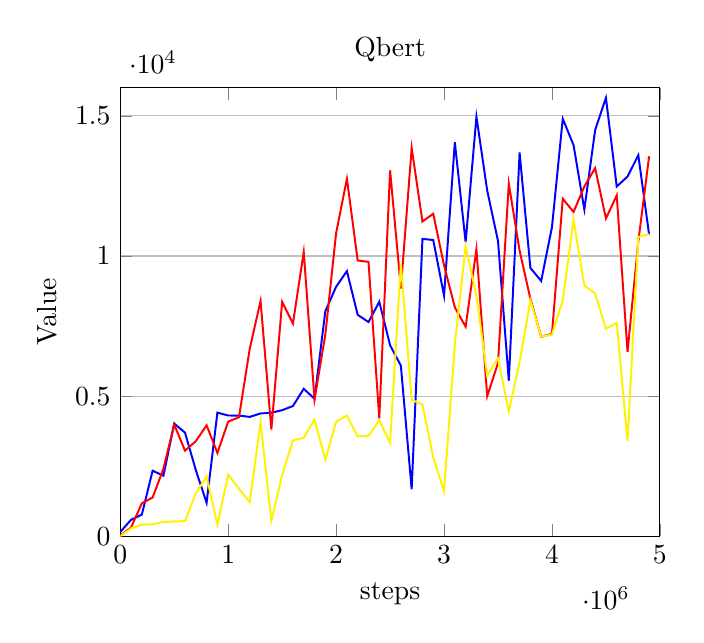
\begin{tikzpicture}

\begin{axis}[%
title=Qbert,
% %width=4.634in,
%width=10in,
%height=5in,
%at={(2.596in,2.358in)},
% scale only axis,
xmin=0,
xmax=5000000,
xlabel style={font=\color{white!15!black}},
xlabel={steps},
xlabel near ticks,
ymin=0,
ymax=16000,
ylabel style={font=\color{white!15!black}},
ylabel={Value},
ylabel near ticks,
ymajorgrids,
% %scale=0.5,
%scale=0.4,
axis background/.style={fill=white},
%legend style={legend cell align=left, align=left, draw=white!15!black}
]
\addplot [color=blue, line width = 0.25mm]
                table[row sep=crcr]{
                  0 150.0\\ 
100000 585.0\\ 
200000 772.5\\ 
300000 2337.5\\ 
400000 2157.5\\ 
500000 4022.5\\ 
600000 3695.0\\ 
700000 2362.5\\ 
800000 1192.5\\ 
900000 4410.0\\ 
1000000 4307.5\\ 
1100000 4305.0\\ 
1200000 4257.5\\ 
1300000 4380.0\\ 
1400000 4407.5\\ 
1500000 4497.5\\ 
1600000 4645.0\\ 
1700000 5260.0\\ 
1800000 4905.0\\ 
1900000 8030.0\\ 
2000000 8902.5\\ 
2100000 9460.0\\ 
2200000 7900.0\\ 
2300000 7642.5\\ 
2400000 8367.5\\ 
2500000 6815.0\\ 
2600000 6085.0\\ 
2700000 1677.5\\ 
2800000 10610.0\\ 
2900000 10570.0\\ 
3000000 8585.0\\ 
3100000 14057.5\\ 
3200000 10490.0\\ 
3300000 14970.0\\ 
3400000 12332.5\\ 
3500000 10537.5\\ 
3600000 5550.0\\ 
3700000 13692.5\\ 
3800000 9572.5\\ 
3900000 9110.0\\ 
4000000 11030.0\\ 
4100000 14897.5\\ 
4200000 13955.0\\ 
4300000 11660.0\\ 
4400000 14495.0\\ 
4500000 15645.0\\ 
4600000 12480.0\\ 
4700000 12835.0\\ 
4800000 13597.5\\ 
4900000 10762.5\\ 
};
\addplot [color=red, line width = 0.25mm]
                table[row sep=crcr]{
                  0 22.5\\ 
100000 310.0\\ 
200000 1172.5\\ 
300000 1382.5\\ 
400000 2410.0\\ 
500000 3982.5\\ 
600000 3052.5\\ 
700000 3390.0\\ 
800000 3957.5\\ 
900000 2970.0\\ 
1000000 4090.0\\ 
1100000 4245.0\\ 
1200000 6697.5\\ 
1300000 8395.0\\ 
1400000 3807.5\\ 
1500000 8360.0\\ 
1600000 7590.0\\ 
1700000 10142.5\\ 
1800000 4877.5\\ 
1900000 7190.0\\ 
2000000 10817.5\\ 
2100000 12755.0\\ 
2200000 9840.0\\ 
2300000 9790.0\\ 
2400000 4202.5\\ 
2500000 13057.5\\ 
2600000 8842.5\\ 
2700000 13852.5\\ 
2800000 11230.0\\ 
2900000 11507.5\\ 
3000000 9665.0\\ 
3100000 8167.5\\ 
3200000 7475.0\\ 
3300000 10242.5\\ 
3400000 4997.5\\ 
3500000 6180.0\\ 
3600000 12582.5\\ 
3700000 10190.0\\ 
3800000 8475.0\\ 
3900000 7115.0\\ 
4000000 7222.5\\ 
4100000 12042.5\\ 
4200000 11572.5\\ 
4300000 12480.0\\ 
4400000 13137.5\\ 
4500000 11337.5\\ 
4600000 12165.0\\ 
4700000 6580.0\\ 
4800000 10517.5\\ 
4900000 13560.0\\ 
};
\addplot [color=yellow, line width = 0.25mm]
                table[row sep=crcr]{
                  0 0.0\\ 
100000 280.0\\ 
200000 415.0\\ 
300000 425.0\\ 
400000 507.5\\ 
500000 525.0\\ 
600000 537.5\\ 
700000 1525.0\\ 
800000 2137.5\\ 
900000 407.5\\ 
1000000 2195.0\\ 
1100000 1690.0\\ 
1200000 1215.0\\ 
1300000 4077.5\\ 
1400000 550.0\\ 
1500000 2185.0\\ 
1600000 3417.5\\ 
1700000 3512.5\\ 
1800000 4165.0\\ 
1900000 2730.0\\ 
2000000 4090.0\\ 
2100000 4305.0\\ 
2200000 3557.5\\ 
2300000 3585.0\\ 
2400000 4137.5\\ 
2500000 3335.0\\ 
2600000 9722.5\\ 
2700000 4865.0\\ 
2800000 4700.0\\ 
2900000 2812.5\\ 
3000000 1605.0\\ 
3100000 6847.5\\ 
3200000 10342.5\\ 
3300000 8590.0\\ 
3400000 5732.5\\ 
3500000 6345.0\\ 
3600000 4447.5\\ 
3700000 6217.5\\ 
3800000 8415.0\\ 
3900000 7120.0\\ 
4000000 7195.0\\ 
4100000 8415.0\\ 
4200000 11307.5\\ 
4300000 8942.5\\ 
4400000 8662.5\\ 
4500000 7402.5\\ 
4600000 7612.5\\ 
4700000 3395.0\\ 
4800000 10680.0\\ 
4900000 10780.0\\ 
};
\end{axis}
\end{tikzpicture}}}
    \subfloat[]{  \resizebox{0.4\textwidth}{!}{
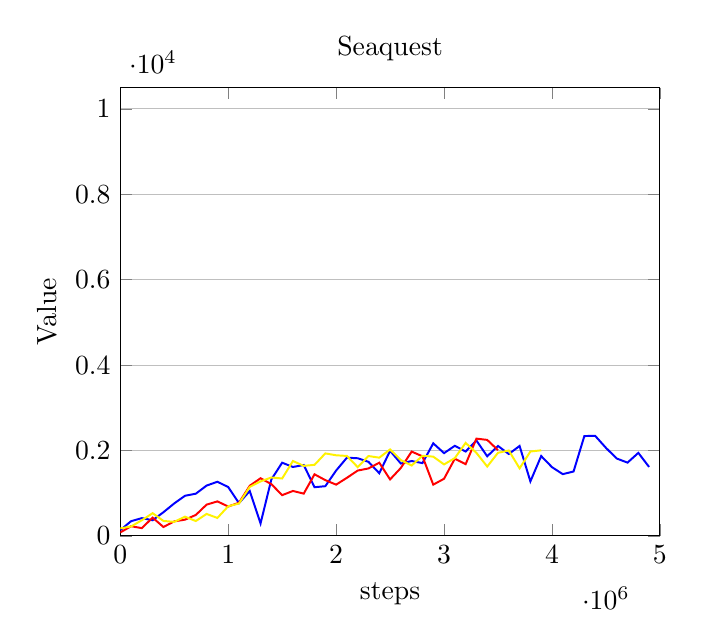
\begin{tikzpicture}

\begin{axis}[%
title=Seaquest,
% %width=4.634in,
%width=10in,
%height=5in,
%at={(2.596in,2.358in)},
% scale only axis,
xmin=0,
xmax=5000000,
xlabel style={font=\color{white!15!black}},
xlabel={steps},
xlabel near ticks,
ymin=0,
ymax=10500,
ylabel style={font=\color{white!15!black}},
ylabel={Value},
ylabel near ticks,
ymajorgrids,
% %scale=0.5,
%scale=0.4,
axis background/.style={fill=white},
%legend style={legend cell align=left, align=left, draw=white!15!black}
]
\addplot [color=blue, line width = 0.25mm]
                table[row sep=crcr]{
                  0 134.0\\ 
100000 344.0\\ 
200000 416.0\\ 
300000 366.0\\ 
400000 554.0\\ 
500000 760.0\\ 
600000 940.0\\ 
700000 988.0\\ 
800000 1178.0\\ 
900000 1268.0\\ 
1000000 1144.0\\ 
1100000 768.0\\ 
1200000 1052.0\\ 
1300000 292.0\\ 
1400000 1322.0\\ 
1500000 1714.0\\ 
1600000 1614.0\\ 
1700000 1660.0\\ 
1800000 1140.0\\ 
1900000 1164.0\\ 
2000000 1530.0\\ 
2100000 1832.0\\ 
2200000 1818.0\\ 
2300000 1734.0\\ 
2400000 1468.0\\ 
2500000 1992.0\\ 
2600000 1694.0\\ 
2700000 1754.0\\ 
2800000 1704.0\\ 
2900000 2168.0\\ 
3000000 1938.0\\ 
3100000 2110.0\\ 
3200000 1976.0\\ 
3300000 2234.0\\ 
3400000 1864.0\\ 
3500000 2106.0\\ 
3600000 1918.0\\ 
3700000 2106.0\\ 
3800000 1276.0\\ 
3900000 1870.0\\ 
4000000 1610.0\\ 
4100000 1446.0\\ 
4200000 1508.0\\ 
4300000 2338.0\\ 
4400000 2344.0\\ 
4500000 2062.0\\ 
4600000 1812.0\\ 
4700000 1716.0\\ 
4800000 1944.0\\ 
4900000 1614.0\\ 
};
\addplot [color=red, line width = 0.25mm]
                table[row sep=crcr]{
                  0 80.0\\ 
100000 226.0\\ 
200000 182.0\\ 
300000 428.0\\ 
400000 208.0\\ 
500000 340.0\\ 
600000 380.0\\ 
700000 490.0\\ 
800000 732.0\\ 
900000 808.0\\ 
1000000 688.0\\ 
1100000 776.0\\ 
1200000 1174.0\\ 
1300000 1350.0\\ 
1400000 1212.0\\ 
1500000 954.0\\ 
1600000 1052.0\\ 
1700000 990.0\\ 
1800000 1442.0\\ 
1900000 1306.0\\ 
2000000 1200.0\\ 
2100000 1360.0\\ 
2200000 1530.0\\ 
2300000 1580.0\\ 
2400000 1714.0\\ 
2500000 1322.0\\ 
2600000 1592.0\\ 
2700000 1974.0\\ 
2800000 1864.0\\ 
2900000 1200.0\\ 
3000000 1338.0\\ 
3100000 1808.0\\ 
3200000 1680.0\\ 
3300000 2278.0\\ 
3400000 2248.0\\ 
3500000 2008.0\\ 
};
\addplot [color=yellow, line width = 0.25mm]
                table[row sep=crcr]{
                  0 176.0\\ 
100000 220.0\\ 
200000 366.0\\ 
300000 532.0\\ 
400000 350.0\\ 
500000 328.0\\ 
600000 450.0\\ 
700000 348.0\\ 
800000 514.0\\ 
900000 420.0\\ 
1000000 694.0\\ 
1100000 758.0\\ 
1200000 1148.0\\ 
1300000 1276.0\\ 
1400000 1368.0\\ 
1500000 1344.0\\ 
1600000 1754.0\\ 
1700000 1640.0\\ 
1800000 1664.0\\ 
1900000 1932.0\\ 
2000000 1888.0\\ 
2100000 1872.0\\ 
2200000 1610.0\\ 
2300000 1870.0\\ 
2400000 1832.0\\ 
2500000 2024.0\\ 
2600000 1774.0\\ 
2700000 1648.0\\ 
2800000 1876.0\\ 
2900000 1856.0\\ 
3000000 1674.0\\ 
3100000 1822.0\\ 
3200000 2178.0\\ 
3300000 1944.0\\ 
3400000 1624.0\\ 
3500000 1946.0\\ 
3600000 2000.0\\ 
3700000 1582.0\\ 
3800000 1976.0\\ 
3900000 2004.0\\ 
};
\end{axis}
\end{tikzpicture}}}\\
  \vspace{-1cm}
    \subfloat[]{  \resizebox{0.4\textwidth}{!}{
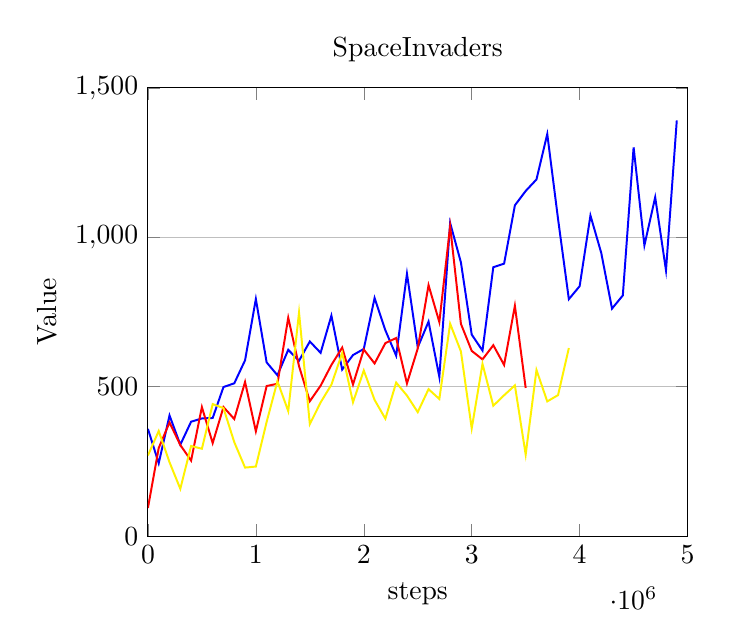
\begin{tikzpicture}

\begin{axis}[%
title=SpaceInvaders,
%width=10in,
%height=5in,
%at={(2.596in,2.358in)},
% scale only axis,
xmin=0,
xmax=5000000,
xlabel style={font=\color{white!15!black}},
xlabel={steps},
xlabel near ticks,
ymin=0,
ymax=1500,
ylabel style={font=\color{white!15!black}},
ylabel={Value},
ylabel near ticks,
ymajorgrids,
% %scale=0.5,
%scale=0.4,
axis background/.style={fill=white},
%legend style={legend cell align=left, align=left, draw=white!15!black}
]
\addplot [color=blue, line width = 0.25mm]
                table[row sep=crcr]{
                  0 359.0\\ 
100000 244.0\\ 
200000 404.0\\ 
300000 306.0\\ 
400000 383.0\\ 
500000 394.0\\ 
600000 395.5\\ 
700000 499.0\\ 
800000 511.5\\ 
900000 588.5\\ 
1000000 793.5\\ 
1100000 581.5\\ 
1200000 538.5\\ 
1300000 623.5\\ 
1400000 587.0\\ 
1500000 651.5\\ 
1600000 613.5\\ 
1700000 738.0\\ 
1800000 557.5\\ 
1900000 606.0\\ 
2000000 626.5\\ 
2100000 797.0\\ 
2200000 689.0\\ 
2300000 604.0\\ 
2400000 878.0\\ 
2500000 632.0\\ 
2600000 718.0\\ 
2700000 533.0\\ 
2800000 1048.0\\ 
2900000 916.0\\ 
3000000 674.5\\ 
3100000 621.0\\ 
3200000 900.0\\ 
3300000 912.0\\ 
3400000 1107.0\\ 
3500000 1155.0\\ 
3600000 1193.5\\ 
3700000 1345.5\\ 
3800000 1061.0\\ 
3900000 793.0\\ 
4000000 836.5\\ 
4100000 1073.0\\ 
4200000 948.0\\ 
4300000 761.5\\ 
4400000 805.5\\ 
4500000 1301.0\\ 
4600000 973.0\\ 
4700000 1134.0\\ 
4800000 889.5\\ 
4900000 1391.0\\ 
};
\addplot [color=red, line width = 0.25mm]
                table[row sep=crcr]{
                  0 94.5\\ 
100000 295.0\\ 
200000 380.5\\ 
300000 305.0\\ 
400000 253.0\\ 
500000 432.0\\ 
600000 311.5\\ 
700000 432.0\\ 
800000 392.0\\ 
900000 516.0\\ 
1000000 351.0\\ 
1100000 502.5\\ 
1200000 510.0\\ 
1300000 731.0\\ 
1400000 569.0\\ 
1500000 451.5\\ 
1600000 503.5\\ 
1700000 573.0\\ 
1800000 631.0\\ 
1900000 507.5\\ 
2000000 624.5\\ 
2100000 578.0\\ 
2200000 646.0\\ 
2300000 663.0\\ 
2400000 511.0\\ 
2500000 628.0\\ 
2600000 840.0\\ 
2700000 716.5\\ 
2800000 1037.0\\ 
2900000 710.5\\ 
3000000 620.0\\ 
3100000 591.5\\ 
3200000 639.0\\ 
3300000 573.0\\ 
3400000 771.0\\ 
3500000 496.0\\ 
};
\addplot [color=yellow, line width = 0.25mm]
                table[row sep=crcr]{
                  0 270.0\\ 
100000 352.0\\ 
200000 247.5\\ 
300000 158.5\\ 
400000 302.0\\ 
500000 292.5\\ 
600000 442.0\\ 
700000 428.5\\ 
800000 314.5\\ 
900000 229.5\\ 
1000000 233.0\\ 
1100000 382.5\\ 
1200000 518.5\\ 
1300000 418.5\\ 
1400000 748.5\\ 
1500000 375.0\\ 
1600000 447.5\\ 
1700000 507.0\\ 
1800000 613.0\\ 
1900000 448.0\\ 
2000000 554.5\\ 
2100000 456.0\\ 
2200000 393.0\\ 
2300000 514.0\\ 
2400000 470.5\\ 
2500000 415.0\\ 
2600000 492.0\\ 
2700000 459.0\\ 
2800000 711.0\\ 
2900000 618.0\\ 
3000000 360.5\\ 
3100000 576.5\\ 
3200000 436.5\\ 
3300000 471.5\\ 
3400000 504.5\\ 
3500000 273.0\\ 
3600000 556.0\\ 
3700000 451.0\\ 
3800000 472.0\\ 
3900000 629.5\\ 
};
\end{axis}
\end{tikzpicture}}}
  \\
    \ref{named}
\end{figure}
\end{frame}


\section{Discussion}

\begin{frame}{Key questions}
		\begin{itemize}
		\item What are the differences between features and states 
				and how important are they to the final performance?
		\item Why is reconstruction loss particularly bad at representing
				stateful information?
		\item What could be the characteristics of more successful approaches
				to using unsupervised learning for state representation learning?
		\item What role does regularization play in reinforcement learning,
				unsupervised learning and their combination?
		\end{itemize}
\end{frame}


\begin{frame}{Differences between features and states}
		\begin{itemize}
				\item in Atari games states are primarily positions and velocities of objects
		\end{itemize}

	\begin{alertblock}{Representation learning methods do not learn this}
			Thus, to work as intended they should either be specialized to the problem,
			or truly made general across many problems.
		%Alert \alert{text}.
	\end{alertblock}
		\begin{itemize}
				\item better understanding of what neural network features are 
						would greatly help in designing them
		\end{itemize}
\pause
	\begin{exampleblock}{Incentivising learning stateful information helps}
			Despite an order of magnitude large unsupervised loss (also destabilizes),
			forward prediction makes a difference.
	\end{exampleblock}
	
\end{frame}

\begin{frame}{Reconstruction loss is bad}
	\begin{alertblock}{Reconstruction loss is ill-suited for state representation learning}
			\begin{itemize}
					\item MSE loss misses important details
					\item MSE loss learns unimportant details
			\end{itemize}
	\end{alertblock}
	\pause
	\begin{exampleblock}{Discriminative models are more promising}
			\begin{itemize}
					\item they allow for better losses
					\item are less computationally expensive
			\end{itemize}
	\end{exampleblock}
	
\end{frame}

\begin{frame}{Not all regularization is the same}
	\begin{alertblock}{Data augmentation hurt joint learning}
			Although it, interestingly, did not hurt either reinforcement 
			nor representation learning individually.
	\end{alertblock}
	\pause
	\begin{exampleblock}{L2 regularization provided a small benefit}
			 Tested separately, it made the reconstruction features more stable,
			 but that was not crucial.
	\end{exampleblock}
	
\end{frame}

\section{Conclusion}

\begin{frame}{Conclusion}
	\begin{alertblock}{Our approach did not work}
			Simply adding pixel reconstruction, and other naive approaches 
			do not increase sample-efficiency.
	\end{alertblock}
	\pause
	\begin{exampleblock}{Our implementation and takeaways help further research}
			The pull request will be made once code is cleaned up.
	\end{exampleblock}
		
\end{frame}

\begin{frame}[focus]
	Thank you for your attention!
\end{frame}







%\begin{frame}[plain]{Plain Slide}
%	This is a slide with the plain style and it is numbered.
%\end{frame}
%
%%------------------------------------------------
%
%\begin{frame}[t]
%	This slide has an empty title and is aligned to top.
%\end{frame}
%
%%------------------------------------------------
%
%\begin{frame}[noframenumbering]{No Slide Numbering}
%	This slide is not numbered and is citing reference \cite{knuth74}.
%\end{frame}
%
%%------------------------------------------------
%
%\begin{frame}{Typesetting and Math}
%	The packages \texttt{inputenc} and \texttt{FiraSans}\footnote{\url{https://fonts.google.com/specimen/Fira+Sans}}\textsuperscript{,}\footnote{\url{http://mozilla.github.io/Fira/}} are used to properly set the main fonts.
%	\vfill
%	This theme provides styling commands to typeset \emph{emphasized}, \alert{alerted}, \textbf{bold}, \textcolor{example}{example text}, \dots
%	\vfill
%	\texttt{FiraSans} also provides support for mathematical symbols:
%	\begin{equation*}
%		e^{i\pi} + 1 = 0.
%	\end{equation*}
%\end{frame}
%
%
%\section{Section 2}
%
%%------------------------------------------------
%
%\begin{frame}{Blocks}
%	These blocks are part of 1 slide, to be displayed consecutively.
%	\begin{block}{Block}
%		Text.
%	\end{block}
%	\pause % Automatically creates a new "page" split between the above and above + below
%	\begin{alertblock}{Alert block}
%		Alert \alert{text}.
%	\end{alertblock}
%	\pause % Automatically creates a new "page" split between the above and above + below
%	\begin{exampleblock}{Example block}
%		Example \textcolor{example}{text}.
%	\end{exampleblock}
%\end{frame}
%
%%------------------------------------------------
%
%\begin{frame}{Columns}
%	\begin{columns}
%		\column{0.5\textwidth}
%			This text appears in the left column and wraps neatly with a margin between columns.
%		
%		\column{0.5\textwidth}
%			
\includegraphics[width=\linewidth]{Images/placeholder.jpg}
%	\end{columns}
%\end{frame}
%
%%------------------------------------------------
%
%\begin{frame}{Lists}
%	\begin{columns}[T, onlytextwidth] % T for top align, onlytextwidth to suppress the margin between columns
%		\column{0.33\textwidth}
%			Items:
%			\begin{itemize}
%				\item Item 1
%				\begin{itemize}
%					\item Subitem 1.1
%					\item Subitem 1.2
%				\end{itemize}
%				\item Item 2
%				\item Item 3
%			\end{itemize}
%		
%		\column{0.33\textwidth}
%			Enumerations:
%			\begin{enumerate}
%				\item First
%				\item Second
%				\begin{enumerate}
%					\item Sub-first
%					\item Sub-second
%				\end{enumerate}
%				\item Third
%			\end{enumerate}
%		
%		\column{0.33\textwidth}
%			Descriptions:
%			\begin{description}
%				\item[First] Yes.
%				\item[Second] No.
%			\end{description}
%	\end{columns}
%\end{frame}
%
%%------------------------------------------------
%
%\begin{frame}{Table}
%	\begin{table}
%		\centering % Centre the table on the slide
%		\begin{tabular}{l c}
%			\toprule
%			Discipline & Avg. Salary \\
%			\toprule
%			\textbf{Engineering} & \textbf{\$66,521} \\
%			Computer Sciences & \$60,005\\
%			Mathematics and Sciences & \$61,867\\
%			Business & \$56,720\\
%			Humanities \& Social Sciences & \$56,669\\
%			Agriculture and Natural Resources & \$53,565\\
%			Communications & \$51,448\\
%			\midrule
%			\textbf{Average for All Disciplines} & \textbf{\$58,114}\\
%			\bottomrule
%		\end{tabular}
%	\caption{Table caption}
%	\end{table}
%\end{frame}
%
%%------------------------------------------------


%----------------------------------------------------------------------------------------
%	 CLOSING/SUPPLEMENTARY SLIDES
%----------------------------------------------------------------------------------------

%\appendix

%\begin{frame}{References}
%%	\bibliography{../thesis_text/bibliography.bib}
%%	\bibliographystyle{plain}
%
%%\addcontentsline{toc}
%\addcontentsline{toc}{chapter}{Bibliography}
%\printbibliography
%\end{frame}

%------------------------------------------------

%\begin{frame}{Backup Slide}
%	This is a backup slide, useful to include additional materials to answer questions from the audience.
%	\vfill
%	The package \texttt{appendixnumberbeamer} is used to refrain from numbering appendix slides.
%\end{frame}

%----------------------------------------------------------------------------------------

\end{document}
